\section{Testing}
With the theremin in a usable state, some testing was performed to assess the capabilities and extent to which the product would have to be improved or modified to allow it to be sold commercially. The main area that would need to be improved was the quality of the sound produced.

\subsection{Minimizing Interference}
In order to test the theremin quantitatively, a set-up was built such that no human variation could be included over the duration of the measurement. This involved making a second plate and grounding it to act as the user's hand such that it could be placed a a distant and would remain constant as opposed to a human user who's hand would move, obscuring the results. 

Using this apparatus, it was found that there was still a considerable amount of variation due to human interference simply because someone was near the wire that connected to the plate capacitor to the circuit. Because of the high frequencies involved, the effects of interference become amplified. This is basically the effect that was sought in order that the remote control be possible, but it has more of an effect than was expected on the rest of the circuit.

An attempt to reduce this noise was made using a coaxial cable to connect the plate capacitor and the circuit. Since the coaxial cable has an outer conducting layer, the field near the inner wire connecting the components is greatly reduced and so the interference from outside is also reduced. In order to reduce the effect still further, the distance between the circuit and capacitor could be reduced.

\subsection{Signal Variation}
A large contributing factor to the imperfections in the output signal is due to inaccuracies in the chip. These can be clearly seen in figure~\ref{fig:variations} where a series of measurements of the same signal are overlaid to show the differences. The measurements are of the same signal with no change, taken at 10\,second intervals.

\begin{figure}[htbp]
	\centering
		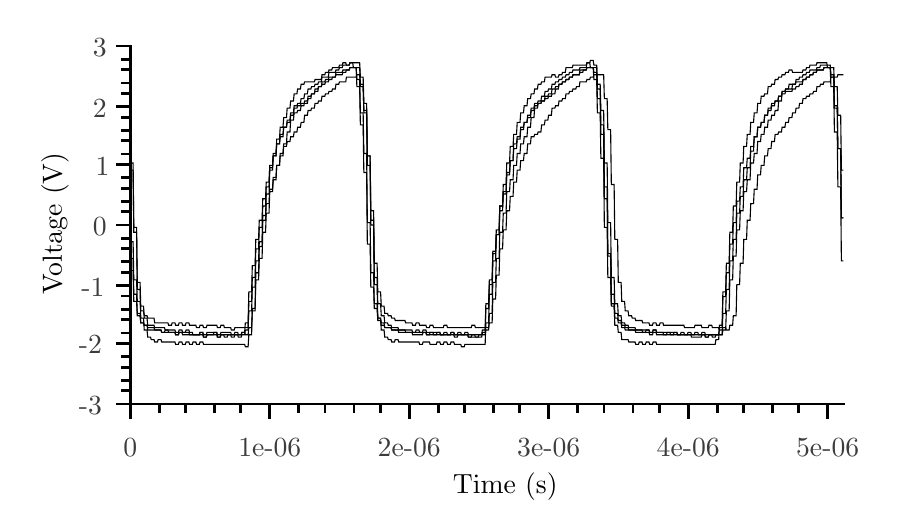
\begin{tikzpicture}{0pt}{0pt}{329pt}{180pt}
	\clip(0pt,180pt) -- (312.853pt,180pt) -- (312.853pt,8.83421pt) -- (0pt,8.83421pt) -- (0pt,180pt);
\begin{scope}
	\clip(37.0859pt,173.344pt) -- (294.786pt,173.344pt) -- (294.786pt,44.0183pt) -- (37.0859pt,44.0183pt) -- (37.0859pt,173.344pt);
	\color[gray]{0}
	\draw[line width=0.4pt, line join=miter, line cap=rect](37.3378pt,96.6106pt) -- (37.5897pt,96.6106pt) -- (37.8416pt,96.6106pt) -- (38.0935pt,96.6106pt) -- (38.3454pt,83.678pt) -- (38.5974pt,83.678pt) -- (38.8493pt,83.678pt) -- (39.1012pt,83.678pt) -- (39.3531pt,83.678pt) -- (39.605pt,76.7807pt) -- (39.8569pt,76.7807pt) -- (40.1088pt,76.7807pt) -- (40.3607pt,76.7807pt) -- (40.6126pt,76.7807pt) -- (40.8645pt,73.332pt) -- (41.1164pt,73.332pt) -- (41.3683pt,73.332pt) -- (41.6202pt,73.332pt) -- (41.8721pt,73.332pt) -- (42.124pt,72.4698pt) -- (42.3759pt,72.4698pt) -- (42.6278pt,72.4698pt) -- (42.8798pt,72.4698pt) -- (43.1317pt,72.4698pt) -- (43.3836pt,70.7455pt) -- (43.6355pt,70.7455pt) -- (43.8874pt,70.7455pt) -- (44.1393pt,70.7455pt) -- (44.3912pt,70.7455pt) -- (44.6431pt,70.7455pt) -- (44.895pt,70.7455pt) -- (45.1469pt,70.7455pt) -- (45.3988pt,70.7455pt) -- (45.6507pt,70.7455pt) -- (45.9026pt,70.7455pt) -- (46.1545pt,70.7455pt) -- (46.4064pt,70.7455pt) -- (46.6583pt,70.7455pt) -- (46.9102pt,70.7455pt) -- (47.1622pt,70.7455pt) -- (47.4141pt,70.7455pt) -- (47.666pt,70.7455pt) -- (47.9179pt,70.7455pt) -- (48.1698pt,70.7455pt) -- (48.4217pt,69.8833pt) -- (48.6736pt,69.8833pt) -- (48.9255pt,69.8833pt) -- (49.1774pt,69.8833pt) -- (49.4293pt,69.8833pt) -- (49.6812pt,69.8833pt) -- (49.9331pt,69.8833pt) -- (50.185pt,69.8833pt) -- (50.4369pt,69.8833pt) -- (50.6888pt,69.8833pt) -- (50.9407pt,69.8833pt) -- (51.1926pt,69.8833pt) -- (51.4446pt,69.8833pt) -- (51.6965pt,69.8833pt) -- (51.9484pt,69.8833pt) -- (52.2003pt,69.8833pt) -- (52.4522pt,69.8833pt) -- (52.7041pt,69.8833pt) -- (52.956pt,69.8833pt) -- (53.2079pt,69.8833pt) -- (53.4598pt,69.0212pt) -- (53.7117pt,69.0212pt) -- (53.9636pt,69.0212pt) -- (54.2155pt,69.0212pt) -- (54.4674pt,69.0212pt) -- (54.7193pt,69.8833pt) -- (54.9712pt,69.8833pt) -- (55.2231pt,69.8833pt) -- (55.475pt,69.8833pt) -- (55.7269pt,69.8833pt) -- (55.9789pt,69.0212pt) -- (56.2308pt,69.0212pt) -- (56.4827pt,69.0212pt) -- (56.7346pt,69.0212pt) -- (56.9865pt,69.0212pt) -- (57.2384pt,69.0212pt) -- (57.4903pt,69.0212pt) -- (57.7422pt,69.0212pt) -- (57.9941pt,69.0212pt) -- (58.246pt,69.0212pt) -- (58.4979pt,69.0212pt) -- (58.7498pt,69.0212pt) -- (59.0017pt,69.0212pt) -- (59.2536pt,69.0212pt) -- (59.5055pt,69.0212pt) -- (59.7574pt,69.0212pt) -- (60.0093pt,69.0212pt) -- (60.2613pt,69.0212pt) -- (60.5132pt,69.0212pt) -- (60.7651pt,69.0212pt) -- (61.017pt,69.0212pt) -- (61.2689pt,69.0212pt) -- (61.5208pt,69.0212pt) -- (61.7727pt,69.0212pt) -- (62.0246pt,69.0212pt) -- (62.2765pt,69.0212pt) -- (62.5284pt,69.0212pt) -- (62.7803pt,69.0212pt) -- (63.0322pt,69.0212pt) -- (63.2841pt,69.0212pt) -- (63.536pt,68.159pt) -- (63.7879pt,68.159pt) -- (64.0398pt,68.159pt) -- (64.2917pt,68.159pt) -- (64.5437pt,68.159pt) -- (64.7956pt,69.0212pt) -- (65.0475pt,69.0212pt) -- (65.2994pt,69.0212pt) -- (65.5513pt,69.0212pt) -- (65.8032pt,69.0212pt) -- (66.0551pt,69.0212pt) -- (66.307pt,69.0212pt) -- (66.5589pt,69.0212pt) -- (66.8108pt,69.0212pt) -- (67.0627pt,69.0212pt) -- (67.3146pt,69.0212pt) -- (67.5665pt,69.0212pt) -- (67.8184pt,69.0212pt) -- (68.0703pt,69.0212pt) -- (68.3222pt,69.0212pt) -- (68.5741pt,68.159pt) -- (68.826pt,68.159pt) -- (69.078pt,68.159pt) -- (69.3299pt,68.159pt) -- (69.5818pt,68.159pt) -- (69.8337pt,69.0212pt) -- (70.0856pt,69.0212pt) -- (70.3375pt,69.0212pt) -- (70.5894pt,69.0212pt) -- (70.8413pt,69.0212pt) -- (71.0932pt,68.159pt) -- (71.3451pt,68.159pt) -- (71.597pt,68.159pt) -- (71.8489pt,68.159pt) -- (72.1008pt,68.159pt) -- (72.3527pt,69.0212pt) -- (72.6046pt,69.0212pt) -- (72.8565pt,69.0212pt) -- (73.1084pt,69.0212pt) -- (73.3604pt,69.0212pt) -- (73.6123pt,68.159pt) -- (73.8642pt,68.159pt) -- (74.1161pt,68.159pt) -- (74.368pt,68.159pt) -- (74.6199pt,68.159pt) -- (74.8718pt,69.0212pt) -- (75.1237pt,69.0212pt) -- (75.3756pt,69.0212pt) -- (75.6275pt,69.0212pt) -- (75.8794pt,69.0212pt) -- (76.1313pt,68.159pt) -- (76.3832pt,68.159pt) -- (76.6351pt,68.159pt) -- (76.887pt,68.159pt) -- (77.1389pt,68.159pt) -- (77.3908pt,69.0212pt) -- (77.6428pt,69.0212pt) -- (77.8947pt,69.0212pt) -- (78.1466pt,69.0212pt) -- (78.3985pt,69.0212pt) -- (78.6504pt,70.7455pt) -- (78.9023pt,70.7455pt) -- (79.1542pt,70.7455pt) -- (79.4061pt,70.7455pt) -- (79.658pt,70.7455pt) -- (79.9099pt,81.0915pt) -- (80.1618pt,81.0915pt) -- (80.4137pt,81.0915pt) -- (80.6656pt,81.0915pt) -- (80.9175pt,81.0915pt) -- (81.1694pt,89.7132pt) -- (81.4213pt,89.7132pt) -- (81.6732pt,89.7132pt) -- (81.9251pt,89.7132pt) -- (82.1771pt,89.7132pt) -- (82.429pt,100.059pt) -- (82.6809pt,100.059pt) -- (82.9328pt,100.059pt) -- (83.1847pt,100.059pt) -- (83.4366pt,100.059pt) -- (83.6885pt,107.819pt) -- (83.9404pt,107.819pt) -- (84.1923pt,107.819pt) -- (84.4442pt,107.819pt) -- (84.6961pt,107.819pt) -- (84.948pt,115.578pt) -- (85.1999pt,115.578pt) -- (85.4518pt,115.578pt) -- (85.7037pt,115.578pt) -- (85.9556pt,115.578pt) -- (86.2075pt,122.476pt) -- (86.4595pt,122.476pt) -- (86.7114pt,122.476pt) -- (86.9633pt,122.476pt) -- (87.2152pt,122.476pt) -- (87.4671pt,130.235pt) -- (87.719pt,130.235pt) -- (87.9709pt,130.235pt) -- (88.2228pt,130.235pt) -- (88.4747pt,130.235pt) -- (88.7266pt,134.546pt) -- (88.9785pt,134.546pt) -- (89.2304pt,134.546pt) -- (89.4823pt,134.546pt) -- (89.7342pt,134.546pt) -- (89.9861pt,137.995pt) -- (90.238pt,137.995pt) -- (90.4899pt,137.995pt) -- (90.7419pt,137.995pt) -- (90.9938pt,137.995pt) -- (91.2457pt,141.443pt) -- (91.4976pt,141.443pt) -- (91.7495pt,141.443pt) -- (92.0014pt,141.443pt) -- (92.2533pt,141.443pt) -- (92.5052pt,144.03pt) -- (92.7571pt,144.03pt) -- (93.009pt,144.03pt) -- (93.2609pt,144.03pt) -- (93.5128pt,144.03pt) -- (93.7647pt,146.616pt) -- (94.0166pt,146.616pt) -- (94.2685pt,146.616pt) -- (94.5204pt,146.616pt) -- (94.7723pt,146.616pt) -- (95.0242pt,149.203pt) -- (95.2762pt,149.203pt) -- (95.5281pt,149.203pt) -- (95.78pt,149.203pt) -- (96.0319pt,149.203pt) -- (96.2838pt,151.789pt) -- (96.5357pt,151.789pt) -- (96.7876pt,151.789pt) -- (97.0395pt,151.789pt) -- (97.2914pt,151.789pt) -- (97.5433pt,152.652pt) -- (97.7952pt,152.652pt) -- (98.0471pt,152.652pt) -- (98.299pt,152.652pt) -- (98.5509pt,152.652pt) -- (98.8028pt,154.376pt) -- (99.0547pt,154.376pt) -- (99.3066pt,154.376pt) -- (99.5586pt,154.376pt) -- (99.8105pt,154.376pt) -- (100.062pt,156.1pt) -- (100.314pt,156.1pt) -- (100.566pt,156.1pt) -- (100.818pt,156.1pt) -- (101.07pt,156.1pt) -- (101.322pt,157.825pt) -- (101.574pt,157.825pt) -- (101.826pt,157.825pt) -- (102.078pt,157.825pt) -- (102.33pt,157.825pt) -- (102.581pt,158.687pt) -- (102.833pt,158.687pt) -- (103.085pt,158.687pt) -- (103.337pt,158.687pt) -- (103.589pt,158.687pt) -- (103.841pt,159.549pt) -- (104.093pt,159.549pt) -- (104.345pt,159.549pt) -- (104.597pt,159.549pt) -- (104.849pt,159.549pt) -- (105.1pt,160.411pt) -- (105.352pt,160.411pt) -- (105.604pt,160.411pt) -- (105.856pt,160.411pt) -- (106.108pt,160.411pt) -- (106.36pt,162.135pt) -- (106.612pt,162.135pt) -- (106.864pt,162.135pt) -- (107.116pt,162.135pt) -- (107.368pt,162.135pt) -- (107.62pt,162.135pt) -- (107.871pt,162.135pt) -- (108.123pt,162.135pt) -- (108.375pt,162.135pt) -- (108.627pt,162.135pt) -- (108.879pt,163.86pt) -- (109.131pt,163.86pt) -- (109.383pt,163.86pt) -- (109.635pt,163.86pt) -- (109.887pt,163.86pt) -- (110.139pt,163.86pt) -- (110.391pt,163.86pt) -- (110.642pt,163.86pt) -- (110.894pt,163.86pt) -- (111.146pt,163.86pt) -- (111.398pt,164.722pt) -- (111.65pt,164.722pt) -- (111.902pt,164.722pt) -- (112.154pt,164.722pt) -- (112.406pt,164.722pt) -- (112.658pt,165.584pt) -- (112.91pt,165.584pt) -- (113.161pt,165.584pt) -- (113.413pt,165.584pt) -- (113.665pt,165.584pt) -- (113.917pt,166.446pt) -- (114.169pt,166.446pt) -- (114.421pt,166.446pt) -- (114.673pt,166.446pt) -- (114.925pt,166.446pt) -- (115.177pt,166.446pt) -- (115.429pt,166.446pt) -- (115.681pt,166.446pt) -- (115.932pt,166.446pt) -- (116.184pt,166.446pt) -- (116.436pt,167.308pt) -- (116.688pt,167.308pt) -- (116.94pt,167.308pt) -- (117.192pt,167.308pt) -- (117.444pt,167.308pt) -- (117.696pt,165.584pt) -- (117.948pt,165.584pt) -- (118.2pt,165.584pt) -- (118.451pt,165.584pt) -- (118.703pt,165.584pt) -- (118.955pt,158.687pt) -- (119.207pt,158.687pt) -- (119.459pt,158.687pt) -- (119.711pt,158.687pt) -- (119.963pt,158.687pt) -- (120.215pt,144.892pt) -- (120.467pt,144.892pt) -- (120.719pt,144.892pt) -- (120.971pt,144.892pt) -- (121.222pt,144.892pt) -- (121.474pt,127.649pt) -- (121.726pt,127.649pt) -- (121.978pt,127.649pt) -- (122.23pt,127.649pt) -- (122.482pt,127.649pt) -- (122.734pt,101.784pt) -- (122.986pt,101.784pt) -- (123.238pt,101.784pt) -- (123.49pt,101.784pt) -- (123.742pt,101.784pt) -- (123.993pt,86.2645pt) -- (124.245pt,86.2645pt) -- (124.497pt,86.2645pt) -- (124.749pt,86.2645pt) -- (125.001pt,86.2645pt) -- (125.253pt,78.505pt) -- (125.505pt,78.505pt) -- (125.757pt,78.505pt) -- (126.009pt,78.505pt) -- (126.261pt,78.505pt) -- (126.512pt,74.1942pt) -- (126.764pt,74.1942pt) -- (127.016pt,74.1942pt) -- (127.268pt,74.1942pt) -- (127.52pt,74.1942pt) -- (127.772pt,72.4698pt) -- (128.024pt,72.4698pt) -- (128.276pt,72.4698pt) -- (128.528pt,72.4698pt) -- (128.78pt,72.4698pt) -- (129.032pt,71.6077pt) -- (129.283pt,71.6077pt) -- (129.535pt,71.6077pt) -- (129.787pt,71.6077pt) -- (130.039pt,71.6077pt) -- (130.291pt,71.6077pt) -- (130.543pt,71.6077pt) -- (130.795pt,71.6077pt) -- (131.047pt,71.6077pt) -- (131.299pt,71.6077pt) -- (131.551pt,70.7455pt) -- (131.802pt,70.7455pt) -- (132.054pt,70.7455pt) -- (132.306pt,70.7455pt) -- (132.558pt,70.7455pt) -- (132.81pt,70.7455pt) -- (133.062pt,70.7455pt) -- (133.314pt,70.7455pt) -- (133.566pt,70.7455pt) -- (133.818pt,70.7455pt) -- (134.07pt,69.8833pt) -- (134.322pt,69.8833pt) -- (134.573pt,69.8833pt) -- (134.825pt,69.8833pt) -- (135.077pt,69.8833pt) -- (135.329pt,69.8833pt) -- (135.581pt,69.8833pt) -- (135.833pt,69.8833pt) -- (136.085pt,69.8833pt) -- (136.337pt,69.8833pt) -- (136.589pt,69.8833pt) -- (136.841pt,69.8833pt) -- (137.093pt,69.8833pt) -- (137.344pt,69.8833pt) -- (137.596pt,69.8833pt) -- (137.848pt,69.8833pt) -- (138.1pt,69.8833pt) -- (138.352pt,69.8833pt) -- (138.604pt,69.8833pt) -- (138.856pt,69.8833pt) -- (139.108pt,69.0212pt) -- (139.36pt,69.0212pt) -- (139.612pt,69.0212pt) -- (139.863pt,69.0212pt) -- (140.115pt,69.0212pt) -- (140.367pt,69.0212pt) -- (140.619pt,69.0212pt) -- (140.871pt,69.0212pt) -- (141.123pt,69.0212pt) -- (141.375pt,69.0212pt) -- (141.627pt,69.0212pt) -- (141.879pt,69.0212pt) -- (142.131pt,69.0212pt) -- (142.383pt,69.0212pt) -- (142.634pt,69.0212pt) -- (142.886pt,69.8833pt) -- (143.138pt,69.8833pt) -- (143.39pt,69.8833pt) -- (143.642pt,69.8833pt) -- (143.894pt,69.8833pt) -- (144.146pt,69.0212pt) -- (144.398pt,69.0212pt) -- (144.65pt,69.0212pt) -- (144.902pt,69.0212pt) -- (145.153pt,69.0212pt) -- (145.405pt,69.0212pt) -- (145.657pt,69.0212pt) -- (145.909pt,69.0212pt) -- (146.161pt,69.0212pt) -- (146.413pt,69.0212pt) -- (146.665pt,69.0212pt) -- (146.917pt,69.0212pt) -- (147.169pt,69.0212pt) -- (147.421pt,69.0212pt) -- (147.673pt,69.0212pt) -- (147.924pt,69.0212pt) -- (148.176pt,69.0212pt) -- (148.428pt,69.0212pt) -- (148.68pt,69.0212pt) -- (148.932pt,69.0212pt) -- (149.184pt,69.0212pt) -- (149.436pt,69.0212pt) -- (149.688pt,69.0212pt) -- (149.94pt,69.0212pt) -- (150.192pt,69.0212pt) -- (150.444pt,69.0212pt) -- (150.695pt,69.0212pt) -- (150.947pt,69.0212pt) -- (151.199pt,69.0212pt) -- (151.451pt,69.0212pt) -- (151.703pt,69.0212pt) -- (151.955pt,69.0212pt) -- (152.207pt,69.0212pt) -- (152.459pt,69.0212pt) -- (152.711pt,69.0212pt) -- (152.963pt,69.0212pt) -- (153.214pt,69.0212pt) -- (153.466pt,69.0212pt) -- (153.718pt,69.0212pt) -- (153.97pt,69.0212pt) -- (154.222pt,68.159pt) -- (154.474pt,68.159pt) -- (154.726pt,68.159pt) -- (154.978pt,68.159pt) -- (155.23pt,68.159pt) -- (155.482pt,69.0212pt) -- (155.734pt,69.0212pt) -- (155.985pt,69.0212pt) -- (156.237pt,69.0212pt) -- (156.489pt,69.0212pt) -- (156.741pt,69.0212pt) -- (156.993pt,69.0212pt) -- (157.245pt,69.0212pt) -- (157.497pt,69.0212pt) -- (157.749pt,69.0212pt) -- (158.001pt,69.0212pt) -- (158.253pt,69.0212pt) -- (158.505pt,69.0212pt) -- (158.756pt,69.0212pt) -- (159.008pt,69.0212pt) -- (159.26pt,68.159pt) -- (159.512pt,68.159pt) -- (159.764pt,68.159pt) -- (160.016pt,68.159pt) -- (160.268pt,68.159pt) -- (160.52pt,68.159pt) -- (160.772pt,68.159pt) -- (161.024pt,68.159pt) -- (161.275pt,68.159pt) -- (161.527pt,68.159pt) -- (161.779pt,68.159pt) -- (162.031pt,68.159pt) -- (162.283pt,68.159pt) -- (162.535pt,68.159pt) -- (162.787pt,68.159pt) -- (163.039pt,68.159pt) -- (163.291pt,68.159pt) -- (163.543pt,68.159pt) -- (163.795pt,68.159pt) -- (164.046pt,68.159pt) -- (164.298pt,69.8833pt) -- (164.55pt,69.8833pt) -- (164.802pt,69.8833pt) -- (165.054pt,69.8833pt) -- (165.306pt,69.8833pt) -- (165.558pt,78.505pt) -- (165.81pt,78.505pt) -- (166.062pt,78.505pt) -- (166.314pt,78.505pt) -- (166.565pt,78.505pt) -- (166.817pt,87.1267pt) -- (167.069pt,87.1267pt) -- (167.321pt,87.1267pt) -- (167.573pt,87.1267pt) -- (167.825pt,87.1267pt) -- (168.077pt,98.3349pt) -- (168.329pt,98.3349pt) -- (168.581pt,98.3349pt) -- (168.833pt,98.3349pt) -- (169.085pt,98.3349pt) -- (169.336pt,105.232pt) -- (169.588pt,105.232pt) -- (169.84pt,105.232pt) -- (170.092pt,105.232pt) -- (170.344pt,105.232pt) -- (170.596pt,113.854pt) -- (170.848pt,113.854pt) -- (171.1pt,113.854pt) -- (171.352pt,113.854pt) -- (171.604pt,113.854pt) -- (171.856pt,119.889pt) -- (172.107pt,119.889pt) -- (172.359pt,119.889pt) -- (172.611pt,119.889pt) -- (172.863pt,119.889pt) -- (173.115pt,126.786pt) -- (173.367pt,126.786pt) -- (173.619pt,126.786pt) -- (173.871pt,126.786pt) -- (174.123pt,126.786pt) -- (174.375pt,131.959pt) -- (174.626pt,131.959pt) -- (174.878pt,131.959pt) -- (175.13pt,131.959pt) -- (175.382pt,131.959pt) -- (175.634pt,137.995pt) -- (175.886pt,137.995pt) -- (176.138pt,137.995pt) -- (176.39pt,137.995pt) -- (176.642pt,137.995pt) -- (176.894pt,140.581pt) -- (177.146pt,140.581pt) -- (177.397pt,140.581pt) -- (177.649pt,140.581pt) -- (177.901pt,140.581pt) -- (178.153pt,144.03pt) -- (178.405pt,144.03pt) -- (178.657pt,144.03pt) -- (178.909pt,144.03pt) -- (179.161pt,144.03pt) -- (179.413pt,145.754pt) -- (179.665pt,145.754pt) -- (179.916pt,145.754pt) -- (180.168pt,145.754pt) -- (180.42pt,145.754pt) -- (180.672pt,148.341pt) -- (180.924pt,148.341pt) -- (181.176pt,148.341pt) -- (181.428pt,148.341pt) -- (181.68pt,148.341pt) -- (181.932pt,150.927pt) -- (182.184pt,150.927pt) -- (182.436pt,150.927pt) -- (182.687pt,150.927pt) -- (182.939pt,150.927pt) -- (183.191pt,152.652pt) -- (183.443pt,152.652pt) -- (183.695pt,152.652pt) -- (183.947pt,152.652pt) -- (184.199pt,152.652pt) -- (184.451pt,153.514pt) -- (184.703pt,153.514pt) -- (184.955pt,153.514pt) -- (185.207pt,153.514pt) -- (185.458pt,153.514pt) -- (185.71pt,155.238pt) -- (185.962pt,155.238pt) -- (186.214pt,155.238pt) -- (186.466pt,155.238pt) -- (186.718pt,155.238pt) -- (186.97pt,156.962pt) -- (187.222pt,156.962pt) -- (187.474pt,156.962pt) -- (187.726pt,156.962pt) -- (187.977pt,156.962pt) -- (188.229pt,157.825pt) -- (188.481pt,157.825pt) -- (188.733pt,157.825pt) -- (188.985pt,157.825pt) -- (189.237pt,157.825pt) -- (189.489pt,159.549pt) -- (189.741pt,159.549pt) -- (189.993pt,159.549pt) -- (190.245pt,159.549pt) -- (190.497pt,159.549pt) -- (190.748pt,160.411pt) -- (191pt,160.411pt) -- (191.252pt,160.411pt) -- (191.504pt,160.411pt) -- (191.756pt,160.411pt) -- (192.008pt,161.273pt) -- (192.26pt,161.273pt) -- (192.512pt,161.273pt) -- (192.764pt,161.273pt) -- (193.016pt,161.273pt) -- (193.267pt,162.135pt) -- (193.519pt,162.135pt) -- (193.771pt,162.135pt) -- (194.023pt,162.135pt) -- (194.275pt,162.135pt) -- (194.527pt,162.998pt) -- (194.779pt,162.998pt) -- (195.031pt,162.998pt) -- (195.283pt,162.998pt) -- (195.535pt,162.998pt) -- (195.787pt,163.86pt) -- (196.038pt,163.86pt) -- (196.29pt,163.86pt) -- (196.542pt,163.86pt) -- (196.794pt,163.86pt) -- (197.046pt,164.722pt) -- (197.298pt,164.722pt) -- (197.55pt,164.722pt) -- (197.802pt,164.722pt) -- (198.054pt,164.722pt) -- (198.306pt,164.722pt) -- (198.558pt,164.722pt) -- (198.809pt,164.722pt) -- (199.061pt,164.722pt) -- (199.313pt,164.722pt) -- (199.565pt,165.584pt) -- (199.817pt,165.584pt) -- (200.069pt,165.584pt) -- (200.321pt,165.584pt) -- (200.573pt,165.584pt) -- (200.825pt,165.584pt) -- (201.077pt,165.584pt) -- (201.328pt,165.584pt) -- (201.58pt,165.584pt) -- (201.832pt,165.584pt) -- (202.084pt,167.308pt) -- (202.336pt,167.308pt) -- (202.588pt,167.308pt) -- (202.84pt,167.308pt) -- (203.092pt,167.308pt) -- (203.344pt,165.584pt) -- (203.596pt,165.584pt) -- (203.848pt,165.584pt) -- (204.099pt,165.584pt) -- (204.351pt,165.584pt) -- (204.603pt,161.273pt) -- (204.855pt,161.273pt) -- (205.107pt,161.273pt) -- (205.359pt,161.273pt) -- (205.611pt,161.273pt) -- (205.863pt,149.203pt) -- (206.115pt,149.203pt) -- (206.367pt,149.203pt) -- (206.619pt,149.203pt) -- (206.87pt,149.203pt) -- (207.122pt,132.822pt) -- (207.374pt,132.822pt) -- (207.626pt,132.822pt) -- (207.878pt,132.822pt) -- (208.13pt,132.822pt) -- (208.382pt,107.819pt) -- (208.634pt,107.819pt) -- (208.886pt,107.819pt) -- (209.138pt,107.819pt) -- (209.389pt,107.819pt) -- (209.641pt,89.7132pt) -- (209.893pt,89.7132pt) -- (210.145pt,89.7132pt) -- (210.397pt,89.7132pt) -- (210.649pt,89.7132pt) -- (210.901pt,79.3672pt) -- (211.153pt,79.3672pt) -- (211.405pt,79.3672pt) -- (211.657pt,79.3672pt) -- (211.909pt,79.3672pt) -- (212.16pt,75.0564pt) -- (212.412pt,75.0564pt) -- (212.664pt,75.0564pt) -- (212.916pt,75.0564pt) -- (213.168pt,75.0564pt) -- (213.42pt,73.332pt) -- (213.672pt,73.332pt) -- (213.924pt,73.332pt) -- (214.176pt,73.332pt) -- (214.428pt,73.332pt) -- (214.679pt,71.6077pt) -- (214.931pt,71.6077pt) -- (215.183pt,71.6077pt) -- (215.435pt,71.6077pt) -- (215.687pt,71.6077pt) -- (215.939pt,70.7455pt) -- (216.191pt,70.7455pt) -- (216.443pt,70.7455pt) -- (216.695pt,70.7455pt) -- (216.947pt,70.7455pt) -- (217.199pt,70.7455pt) -- (217.45pt,70.7455pt) -- (217.702pt,70.7455pt) -- (217.954pt,70.7455pt) -- (218.206pt,70.7455pt) -- (218.458pt,70.7455pt) -- (218.71pt,70.7455pt) -- (218.962pt,70.7455pt) -- (219.214pt,70.7455pt) -- (219.466pt,70.7455pt) -- (219.718pt,69.8833pt) -- (219.97pt,69.8833pt) -- (220.221pt,69.8833pt) -- (220.473pt,69.8833pt) -- (220.725pt,69.8833pt) -- (220.977pt,69.8833pt) -- (221.229pt,69.8833pt) -- (221.481pt,69.8833pt) -- (221.733pt,69.8833pt) -- (221.985pt,69.8833pt) -- (222.237pt,69.8833pt) -- (222.489pt,69.8833pt) -- (222.74pt,69.8833pt) -- (222.992pt,69.8833pt) -- (223.244pt,69.8833pt) -- (223.496pt,69.8833pt) -- (223.748pt,69.8833pt) -- (224pt,69.8833pt) -- (224.252pt,69.8833pt) -- (224.504pt,69.8833pt) -- (224.756pt,69.0212pt) -- (225.008pt,69.0212pt) -- (225.26pt,69.0212pt) -- (225.511pt,69.0212pt) -- (225.763pt,69.0212pt) -- (226.015pt,69.8833pt) -- (226.267pt,69.8833pt) -- (226.519pt,69.8833pt) -- (226.771pt,69.8833pt) -- (227.023pt,69.8833pt) -- (227.275pt,69.0212pt) -- (227.527pt,69.0212pt) -- (227.779pt,69.0212pt) -- (228.03pt,69.0212pt) -- (228.282pt,69.0212pt) -- (228.534pt,69.0212pt) -- (228.786pt,69.0212pt) -- (229.038pt,69.0212pt) -- (229.29pt,69.0212pt) -- (229.542pt,69.0212pt) -- (229.794pt,69.0212pt) -- (230.046pt,69.0212pt) -- (230.298pt,69.0212pt) -- (230.55pt,69.0212pt) -- (230.801pt,69.0212pt) -- (231.053pt,69.0212pt) -- (231.305pt,69.0212pt) -- (231.557pt,69.0212pt) -- (231.809pt,69.0212pt) -- (232.061pt,69.0212pt) -- (232.313pt,69.0212pt) -- (232.565pt,69.0212pt) -- (232.817pt,69.0212pt) -- (233.069pt,69.0212pt) -- (233.321pt,69.0212pt) -- (233.572pt,69.0212pt) -- (233.824pt,69.0212pt) -- (234.076pt,69.0212pt) -- (234.328pt,69.0212pt) -- (234.58pt,69.0212pt) -- (234.832pt,69.0212pt) -- (235.084pt,69.0212pt) -- (235.336pt,69.0212pt) -- (235.588pt,69.0212pt) -- (235.84pt,69.0212pt) -- (236.091pt,69.0212pt) -- (236.343pt,69.0212pt) -- (236.595pt,69.0212pt) -- (236.847pt,69.0212pt) -- (237.099pt,69.0212pt) -- (237.351pt,69.0212pt) -- (237.603pt,69.0212pt) -- (237.855pt,69.0212pt) -- (238.107pt,69.0212pt) -- (238.359pt,69.0212pt) -- (238.611pt,69.0212pt) -- (238.862pt,69.0212pt) -- (239.114pt,69.0212pt) -- (239.366pt,69.0212pt) -- (239.618pt,69.0212pt) -- (239.87pt,68.159pt) -- (240.122pt,68.159pt) -- (240.374pt,68.159pt) -- (240.626pt,68.159pt) -- (240.878pt,68.159pt) -- (241.13pt,68.159pt) -- (241.382pt,68.159pt) -- (241.633pt,68.159pt) -- (241.885pt,68.159pt) -- (242.137pt,68.159pt) -- (242.389pt,68.159pt) -- (242.641pt,68.159pt) -- (242.893pt,68.159pt) -- (243.145pt,68.159pt) -- (243.397pt,68.159pt) -- (243.649pt,69.0212pt) -- (243.901pt,69.0212pt) -- (244.152pt,69.0212pt) -- (244.404pt,69.0212pt) -- (244.656pt,69.0212pt) -- (244.908pt,68.159pt) -- (245.16pt,68.159pt) -- (245.412pt,68.159pt) -- (245.664pt,68.159pt) -- (245.916pt,68.159pt) -- (246.168pt,69.0212pt) -- (246.42pt,69.0212pt) -- (246.672pt,69.0212pt) -- (246.923pt,69.0212pt) -- (247.175pt,69.0212pt) -- (247.427pt,68.159pt) -- (247.679pt,68.159pt) -- (247.931pt,68.159pt) -- (248.183pt,68.159pt) -- (248.435pt,68.159pt) -- (248.687pt,69.0212pt) -- (248.939pt,69.0212pt) -- (249.191pt,69.0212pt) -- (249.442pt,69.0212pt) -- (249.694pt,69.0212pt) -- (249.946pt,69.0212pt) -- (250.198pt,69.0212pt) -- (250.45pt,69.0212pt) -- (250.702pt,69.0212pt) -- (250.954pt,69.0212pt) -- (251.206pt,76.7807pt) -- (251.458pt,76.7807pt) -- (251.71pt,76.7807pt) -- (251.962pt,76.7807pt) -- (252.213pt,76.7807pt) -- (252.465pt,85.4024pt) -- (252.717pt,85.4024pt) -- (252.969pt,85.4024pt) -- (253.221pt,85.4024pt) -- (253.473pt,85.4024pt) -- (253.725pt,95.7484pt) -- (253.977pt,95.7484pt) -- (254.229pt,95.7484pt) -- (254.481pt,95.7484pt) -- (254.733pt,95.7484pt) -- (254.984pt,103.508pt) -- (255.236pt,103.508pt) -- (255.488pt,103.508pt) -- (255.74pt,103.508pt) -- (255.992pt,103.508pt) -- (256.244pt,112.992pt) -- (256.496pt,112.992pt) -- (256.748pt,112.992pt) -- (257pt,112.992pt) -- (257.252pt,112.992pt) -- (257.503pt,119.027pt) -- (257.755pt,119.027pt) -- (258.007pt,119.027pt) -- (258.259pt,119.027pt) -- (258.511pt,119.027pt) -- (258.763pt,125.062pt) -- (259.015pt,125.062pt) -- (259.267pt,125.062pt) -- (259.519pt,125.062pt) -- (259.771pt,125.062pt) -- (260.023pt,129.373pt) -- (260.274pt,129.373pt) -- (260.526pt,129.373pt) -- (260.778pt,129.373pt) -- (261.03pt,129.373pt) -- (261.282pt,135.408pt) -- (261.534pt,135.408pt) -- (261.786pt,135.408pt) -- (262.038pt,135.408pt) -- (262.29pt,135.408pt) -- (262.542pt,140.581pt) -- (262.793pt,140.581pt) -- (263.045pt,140.581pt) -- (263.297pt,140.581pt) -- (263.549pt,140.581pt) -- (263.801pt,144.03pt) -- (264.053pt,144.03pt) -- (264.305pt,144.03pt) -- (264.557pt,144.03pt) -- (264.809pt,144.03pt) -- (265.061pt,145.754pt) -- (265.313pt,145.754pt) -- (265.564pt,145.754pt) -- (265.816pt,145.754pt) -- (266.068pt,145.754pt) -- (266.32pt,148.341pt) -- (266.572pt,148.341pt) -- (266.824pt,148.341pt) -- (267.076pt,148.341pt) -- (267.328pt,148.341pt) -- (267.58pt,150.065pt) -- (267.832pt,150.065pt) -- (268.084pt,150.065pt) -- (268.335pt,150.065pt) -- (268.587pt,150.065pt) -- (268.839pt,151.789pt) -- (269.091pt,151.789pt) -- (269.343pt,151.789pt) -- (269.595pt,151.789pt) -- (269.847pt,151.789pt) -- (270.099pt,153.514pt) -- (270.351pt,153.514pt) -- (270.603pt,153.514pt) -- (270.854pt,153.514pt) -- (271.106pt,153.514pt) -- (271.358pt,155.238pt) -- (271.61pt,155.238pt) -- (271.862pt,155.238pt) -- (272.114pt,155.238pt) -- (272.366pt,155.238pt) -- (272.618pt,156.962pt) -- (272.87pt,156.962pt) -- (273.122pt,156.962pt) -- (273.374pt,156.962pt) -- (273.625pt,156.962pt) -- (273.877pt,157.825pt) -- (274.129pt,157.825pt) -- (274.381pt,157.825pt) -- (274.633pt,157.825pt) -- (274.885pt,157.825pt) -- (275.137pt,159.549pt) -- (275.389pt,159.549pt) -- (275.641pt,159.549pt) -- (275.893pt,159.549pt) -- (276.144pt,159.549pt) -- (276.396pt,159.549pt) -- (276.648pt,159.549pt) -- (276.9pt,159.549pt) -- (277.152pt,159.549pt) -- (277.404pt,159.549pt) -- (277.656pt,161.273pt) -- (277.908pt,161.273pt) -- (278.16pt,161.273pt) -- (278.412pt,161.273pt) -- (278.664pt,161.273pt) -- (278.915pt,162.135pt) -- (279.167pt,162.135pt) -- (279.419pt,162.135pt) -- (279.671pt,162.135pt) -- (279.923pt,162.135pt) -- (280.175pt,162.998pt) -- (280.427pt,162.998pt) -- (280.679pt,162.998pt) -- (280.931pt,162.998pt) -- (281.183pt,162.998pt) -- (281.435pt,163.86pt) -- (281.686pt,163.86pt) -- (281.938pt,163.86pt) -- (282.19pt,163.86pt) -- (282.442pt,163.86pt) -- (282.694pt,164.722pt) -- (282.946pt,164.722pt) -- (283.198pt,164.722pt) -- (283.45pt,164.722pt) -- (283.702pt,164.722pt) -- (283.954pt,164.722pt) -- (284.205pt,164.722pt) -- (284.457pt,164.722pt) -- (284.709pt,164.722pt) -- (284.961pt,164.722pt) -- (285.213pt,165.584pt) -- (285.465pt,165.584pt) -- (285.717pt,165.584pt) -- (285.969pt,165.584pt) -- (286.221pt,165.584pt) -- (286.473pt,166.446pt) -- (286.725pt,166.446pt) -- (286.976pt,166.446pt) -- (287.228pt,166.446pt) -- (287.48pt,166.446pt) -- (287.732pt,166.446pt) -- (287.984pt,166.446pt) -- (288.236pt,166.446pt) -- (288.488pt,166.446pt) -- (288.74pt,166.446pt) -- (288.992pt,166.446pt) -- (289.244pt,166.446pt) -- (289.496pt,166.446pt) -- (289.747pt,166.446pt) -- (289.999pt,166.446pt) -- (290.251pt,162.998pt) -- (290.503pt,162.998pt) -- (290.755pt,162.998pt) -- (291.007pt,162.998pt) -- (291.259pt,162.998pt) -- (291.511pt,151.789pt) -- (291.763pt,151.789pt) -- (292.015pt,151.789pt) -- (292.266pt,151.789pt) -- (292.518pt,151.789pt) -- (292.77pt,136.27pt) -- (293.022pt,136.27pt) -- (293.274pt,136.27pt) -- (293.526pt,136.27pt) -- (293.778pt,136.27pt) -- (294.03pt,111.267pt) -- (294.282pt,111.267pt) -- (294.534pt,111.267pt) -- (294.786pt,111.267pt);
	\color[gray]{0}
	\draw[line width=0.4pt, line join=miter, line cap=rect](37.3378pt,92.2997pt) -- (37.5897pt,92.2997pt) -- (37.8416pt,92.2997pt) -- (38.0935pt,92.2997pt) -- (38.3454pt,81.0915pt) -- (38.5974pt,81.0915pt) -- (38.8493pt,81.0915pt) -- (39.1012pt,81.0915pt) -- (39.3531pt,81.0915pt) -- (39.605pt,75.9185pt) -- (39.8569pt,75.9185pt) -- (40.1088pt,75.9185pt) -- (40.3607pt,75.9185pt) -- (40.6126pt,75.9185pt) -- (40.8645pt,73.332pt) -- (41.1164pt,73.332pt) -- (41.3683pt,73.332pt) -- (41.6202pt,73.332pt) -- (41.8721pt,73.332pt) -- (42.124pt,72.4698pt) -- (42.3759pt,72.4698pt) -- (42.6278pt,72.4698pt) -- (42.8798pt,72.4698pt) -- (43.1317pt,72.4698pt) -- (43.3836pt,71.6077pt) -- (43.6355pt,71.6077pt) -- (43.8874pt,71.6077pt) -- (44.1393pt,71.6077pt) -- (44.3912pt,71.6077pt) -- (44.6431pt,71.6077pt) -- (44.895pt,71.6077pt) -- (45.1469pt,71.6077pt) -- (45.3988pt,71.6077pt) -- (45.6507pt,71.6077pt) -- (45.9026pt,70.7455pt) -- (46.1545pt,70.7455pt) -- (46.4064pt,70.7455pt) -- (46.6583pt,70.7455pt) -- (46.9102pt,70.7455pt) -- (47.1622pt,70.7455pt) -- (47.4141pt,70.7455pt) -- (47.666pt,70.7455pt) -- (47.9179pt,70.7455pt) -- (48.1698pt,70.7455pt) -- (48.4217pt,69.8833pt) -- (48.6736pt,69.8833pt) -- (48.9255pt,69.8833pt) -- (49.1774pt,69.8833pt) -- (49.4293pt,69.8833pt) -- (49.6812pt,70.7455pt) -- (49.9331pt,70.7455pt) -- (50.185pt,70.7455pt) -- (50.4369pt,70.7455pt) -- (50.6888pt,70.7455pt) -- (50.9407pt,69.8833pt) -- (51.1926pt,69.8833pt) -- (51.4446pt,69.8833pt) -- (51.6965pt,69.8833pt) -- (51.9484pt,69.8833pt) -- (52.2003pt,69.8833pt) -- (52.4522pt,69.8833pt) -- (52.7041pt,69.8833pt) -- (52.956pt,69.8833pt) -- (53.2079pt,69.8833pt) -- (53.4598pt,69.0212pt) -- (53.7117pt,69.0212pt) -- (53.9636pt,69.0212pt) -- (54.2155pt,69.0212pt) -- (54.4674pt,69.0212pt) -- (54.7193pt,69.8833pt) -- (54.9712pt,69.8833pt) -- (55.2231pt,69.8833pt) -- (55.475pt,69.8833pt) -- (55.7269pt,69.8833pt) -- (55.9789pt,69.8833pt) -- (56.2308pt,69.8833pt) -- (56.4827pt,69.8833pt) -- (56.7346pt,69.8833pt) -- (56.9865pt,69.8833pt) -- (57.2384pt,69.8833pt) -- (57.4903pt,69.8833pt) -- (57.7422pt,69.8833pt) -- (57.9941pt,69.8833pt) -- (58.246pt,69.8833pt) -- (58.4979pt,69.0212pt) -- (58.7498pt,69.0212pt) -- (59.0017pt,69.0212pt) -- (59.2536pt,69.0212pt) -- (59.5055pt,69.0212pt) -- (59.7574pt,69.0212pt) -- (60.0093pt,69.0212pt) -- (60.2613pt,69.0212pt) -- (60.5132pt,69.0212pt) -- (60.7651pt,69.0212pt) -- (61.017pt,69.0212pt) -- (61.2689pt,69.0212pt) -- (61.5208pt,69.0212pt) -- (61.7727pt,69.0212pt) -- (62.0246pt,69.0212pt) -- (62.2765pt,69.8833pt) -- (62.5284pt,69.8833pt) -- (62.7803pt,69.8833pt) -- (63.0322pt,69.8833pt) -- (63.2841pt,69.8833pt) -- (63.536pt,68.159pt) -- (63.7879pt,68.159pt) -- (64.0398pt,68.159pt) -- (64.2917pt,68.159pt) -- (64.5437pt,68.159pt) -- (64.7956pt,69.0212pt) -- (65.0475pt,69.0212pt) -- (65.2994pt,69.0212pt) -- (65.5513pt,69.0212pt) -- (65.8032pt,69.0212pt) -- (66.0551pt,69.0212pt) -- (66.307pt,69.0212pt) -- (66.5589pt,69.0212pt) -- (66.8108pt,69.0212pt) -- (67.0627pt,69.0212pt) -- (67.3146pt,69.8833pt) -- (67.5665pt,69.8833pt) -- (67.8184pt,69.8833pt) -- (68.0703pt,69.8833pt) -- (68.3222pt,69.8833pt) -- (68.5741pt,68.159pt) -- (68.826pt,68.159pt) -- (69.078pt,68.159pt) -- (69.3299pt,68.159pt) -- (69.5818pt,68.159pt) -- (69.8337pt,69.0212pt) -- (70.0856pt,69.0212pt) -- (70.3375pt,69.0212pt) -- (70.5894pt,69.0212pt) -- (70.8413pt,69.0212pt) -- (71.0932pt,69.0212pt) -- (71.3451pt,69.0212pt) -- (71.597pt,69.0212pt) -- (71.8489pt,69.0212pt) -- (72.1008pt,69.0212pt) -- (72.3527pt,69.0212pt) -- (72.6046pt,69.0212pt) -- (72.8565pt,69.0212pt) -- (73.1084pt,69.0212pt) -- (73.3604pt,69.0212pt) -- (73.6123pt,69.0212pt) -- (73.8642pt,69.0212pt) -- (74.1161pt,69.0212pt) -- (74.368pt,69.0212pt) -- (74.6199pt,69.0212pt) -- (74.8718pt,69.0212pt) -- (75.1237pt,69.0212pt) -- (75.3756pt,69.0212pt) -- (75.6275pt,69.0212pt) -- (75.8794pt,69.0212pt) -- (76.1313pt,69.0212pt) -- (76.3832pt,69.0212pt) -- (76.6351pt,69.0212pt) -- (76.887pt,69.0212pt) -- (77.1389pt,69.0212pt) -- (77.3908pt,69.8833pt) -- (77.6428pt,69.8833pt) -- (77.8947pt,69.8833pt) -- (78.1466pt,69.8833pt) -- (78.3985pt,69.8833pt) -- (78.6504pt,73.332pt) -- (78.9023pt,73.332pt) -- (79.1542pt,73.332pt) -- (79.4061pt,73.332pt) -- (79.658pt,73.332pt) -- (79.9099pt,84.5402pt) -- (80.1618pt,84.5402pt) -- (80.4137pt,84.5402pt) -- (80.6656pt,84.5402pt) -- (80.9175pt,84.5402pt) -- (81.1694pt,94.0241pt) -- (81.4213pt,94.0241pt) -- (81.6732pt,94.0241pt) -- (81.9251pt,94.0241pt) -- (82.1771pt,94.0241pt) -- (82.429pt,103.508pt) -- (82.6809pt,103.508pt) -- (82.9328pt,103.508pt) -- (83.1847pt,103.508pt) -- (83.4366pt,103.508pt) -- (83.6885pt,110.405pt) -- (83.9404pt,110.405pt) -- (84.1923pt,110.405pt) -- (84.4442pt,110.405pt) -- (84.6961pt,110.405pt) -- (84.948pt,118.165pt) -- (85.1999pt,118.165pt) -- (85.4518pt,118.165pt) -- (85.7037pt,118.165pt) -- (85.9556pt,118.165pt) -- (86.2075pt,124.2pt) -- (86.4595pt,124.2pt) -- (86.7114pt,124.2pt) -- (86.9633pt,124.2pt) -- (87.2152pt,124.2pt) -- (87.4671pt,129.373pt) -- (87.719pt,129.373pt) -- (87.9709pt,129.373pt) -- (88.2228pt,129.373pt) -- (88.4747pt,129.373pt) -- (88.7266pt,133.684pt) -- (88.9785pt,133.684pt) -- (89.2304pt,133.684pt) -- (89.4823pt,133.684pt) -- (89.7342pt,133.684pt) -- (89.9861pt,137.995pt) -- (90.238pt,137.995pt) -- (90.4899pt,137.995pt) -- (90.7419pt,137.995pt) -- (90.9938pt,137.995pt) -- (91.2457pt,140.581pt) -- (91.4976pt,140.581pt) -- (91.7495pt,140.581pt) -- (92.0014pt,140.581pt) -- (92.2533pt,140.581pt) -- (92.5052pt,144.03pt) -- (92.7571pt,144.03pt) -- (93.009pt,144.03pt) -- (93.2609pt,144.03pt) -- (93.5128pt,144.03pt) -- (93.7647pt,145.754pt) -- (94.0166pt,145.754pt) -- (94.2685pt,145.754pt) -- (94.5204pt,145.754pt) -- (94.7723pt,145.754pt) -- (95.0242pt,148.341pt) -- (95.2762pt,148.341pt) -- (95.5281pt,148.341pt) -- (95.78pt,148.341pt) -- (96.0319pt,148.341pt) -- (96.2838pt,150.927pt) -- (96.5357pt,150.927pt) -- (96.7876pt,150.927pt) -- (97.0395pt,150.927pt) -- (97.2914pt,150.927pt) -- (97.5433pt,151.789pt) -- (97.7952pt,151.789pt) -- (98.0471pt,151.789pt) -- (98.299pt,151.789pt) -- (98.5509pt,151.789pt) -- (98.8028pt,152.652pt) -- (99.0547pt,152.652pt) -- (99.3066pt,152.652pt) -- (99.5586pt,152.652pt) -- (99.8105pt,152.652pt) -- (100.062pt,152.652pt) -- (100.314pt,152.652pt) -- (100.566pt,152.652pt) -- (100.818pt,152.652pt) -- (101.07pt,152.652pt) -- (101.322pt,154.376pt) -- (101.574pt,154.376pt) -- (101.826pt,154.376pt) -- (102.078pt,154.376pt) -- (102.33pt,154.376pt) -- (102.581pt,156.1pt) -- (102.833pt,156.1pt) -- (103.085pt,156.1pt) -- (103.337pt,156.1pt) -- (103.589pt,156.1pt) -- (103.841pt,157.825pt) -- (104.093pt,157.825pt) -- (104.345pt,157.825pt) -- (104.597pt,157.825pt) -- (104.849pt,157.825pt) -- (105.1pt,158.687pt) -- (105.352pt,158.687pt) -- (105.604pt,158.687pt) -- (105.856pt,158.687pt) -- (106.108pt,158.687pt) -- (106.36pt,160.411pt) -- (106.612pt,160.411pt) -- (106.864pt,160.411pt) -- (107.116pt,160.411pt) -- (107.368pt,160.411pt) -- (107.62pt,161.273pt) -- (107.871pt,161.273pt) -- (108.123pt,161.273pt) -- (108.375pt,161.273pt) -- (108.627pt,161.273pt) -- (108.879pt,162.135pt) -- (109.131pt,162.135pt) -- (109.383pt,162.135pt) -- (109.635pt,162.135pt) -- (109.887pt,162.135pt) -- (110.139pt,162.135pt) -- (110.391pt,162.135pt) -- (110.642pt,162.135pt) -- (110.894pt,162.135pt) -- (111.146pt,162.135pt) -- (111.398pt,163.86pt) -- (111.65pt,163.86pt) -- (111.902pt,163.86pt) -- (112.154pt,163.86pt) -- (112.406pt,163.86pt) -- (112.658pt,163.86pt) -- (112.91pt,163.86pt) -- (113.161pt,163.86pt) -- (113.413pt,163.86pt) -- (113.665pt,163.86pt) -- (113.917pt,164.722pt) -- (114.169pt,164.722pt) -- (114.421pt,164.722pt) -- (114.673pt,164.722pt) -- (114.925pt,164.722pt) -- (115.177pt,164.722pt) -- (115.429pt,164.722pt) -- (115.681pt,164.722pt) -- (115.932pt,164.722pt) -- (116.184pt,164.722pt) -- (116.436pt,165.584pt) -- (116.688pt,165.584pt) -- (116.94pt,165.584pt) -- (117.192pt,165.584pt) -- (117.444pt,165.584pt) -- (117.696pt,165.584pt) -- (117.948pt,165.584pt) -- (118.2pt,165.584pt) -- (118.451pt,165.584pt) -- (118.703pt,165.584pt) -- (118.955pt,161.273pt) -- (119.207pt,161.273pt) -- (119.459pt,161.273pt) -- (119.711pt,161.273pt) -- (119.963pt,161.273pt) -- (120.215pt,149.203pt) -- (120.467pt,149.203pt) -- (120.719pt,149.203pt) -- (120.971pt,149.203pt) -- (121.222pt,149.203pt) -- (121.474pt,134.546pt) -- (121.726pt,134.546pt) -- (121.978pt,134.546pt) -- (122.23pt,134.546pt) -- (122.482pt,134.546pt) -- (122.734pt,109.543pt) -- (122.986pt,109.543pt) -- (123.238pt,109.543pt) -- (123.49pt,109.543pt) -- (123.742pt,109.543pt) -- (123.993pt,91.4376pt) -- (124.245pt,91.4376pt) -- (124.497pt,91.4376pt) -- (124.749pt,91.4376pt) -- (125.001pt,91.4376pt) -- (125.253pt,80.2294pt) -- (125.505pt,80.2294pt) -- (125.757pt,80.2294pt) -- (126.009pt,80.2294pt) -- (126.261pt,80.2294pt) -- (126.512pt,75.0564pt) -- (126.764pt,75.0564pt) -- (127.016pt,75.0564pt) -- (127.268pt,75.0564pt) -- (127.52pt,75.0564pt) -- (127.772pt,73.332pt) -- (128.024pt,73.332pt) -- (128.276pt,73.332pt) -- (128.528pt,73.332pt) -- (128.78pt,73.332pt) -- (129.032pt,71.6077pt) -- (129.283pt,71.6077pt) -- (129.535pt,71.6077pt) -- (129.787pt,71.6077pt) -- (130.039pt,71.6077pt) -- (130.291pt,71.6077pt) -- (130.543pt,71.6077pt) -- (130.795pt,71.6077pt) -- (131.047pt,71.6077pt) -- (131.299pt,71.6077pt) -- (131.551pt,70.7455pt) -- (131.802pt,70.7455pt) -- (132.054pt,70.7455pt) -- (132.306pt,70.7455pt) -- (132.558pt,70.7455pt) -- (132.81pt,70.7455pt) -- (133.062pt,70.7455pt) -- (133.314pt,70.7455pt) -- (133.566pt,70.7455pt) -- (133.818pt,70.7455pt) -- (134.07pt,70.7455pt) -- (134.322pt,70.7455pt) -- (134.573pt,70.7455pt) -- (134.825pt,70.7455pt) -- (135.077pt,70.7455pt) -- (135.329pt,70.7455pt) -- (135.581pt,70.7455pt) -- (135.833pt,70.7455pt) -- (136.085pt,70.7455pt) -- (136.337pt,70.7455pt) -- (136.589pt,69.8833pt) -- (136.841pt,69.8833pt) -- (137.093pt,69.8833pt) -- (137.344pt,69.8833pt) -- (137.596pt,69.8833pt) -- (137.848pt,69.8833pt) -- (138.1pt,69.8833pt) -- (138.352pt,69.8833pt) -- (138.604pt,69.8833pt) -- (138.856pt,69.8833pt) -- (139.108pt,69.8833pt) -- (139.36pt,69.8833pt) -- (139.612pt,69.8833pt) -- (139.863pt,69.8833pt) -- (140.115pt,69.8833pt) -- (140.367pt,69.8833pt) -- (140.619pt,69.8833pt) -- (140.871pt,69.8833pt) -- (141.123pt,69.8833pt) -- (141.375pt,69.8833pt) -- (141.627pt,69.8833pt) -- (141.879pt,69.8833pt) -- (142.131pt,69.8833pt) -- (142.383pt,69.8833pt) -- (142.634pt,69.8833pt) -- (142.886pt,69.8833pt) -- (143.138pt,69.8833pt) -- (143.39pt,69.8833pt) -- (143.642pt,69.8833pt) -- (143.894pt,69.8833pt) -- (144.146pt,69.0212pt) -- (144.398pt,69.0212pt) -- (144.65pt,69.0212pt) -- (144.902pt,69.0212pt) -- (145.153pt,69.0212pt) -- (145.405pt,69.8833pt) -- (145.657pt,69.8833pt) -- (145.909pt,69.8833pt) -- (146.161pt,69.8833pt) -- (146.413pt,69.8833pt) -- (146.665pt,69.0212pt) -- (146.917pt,69.0212pt) -- (147.169pt,69.0212pt) -- (147.421pt,69.0212pt) -- (147.673pt,69.0212pt) -- (147.924pt,69.8833pt) -- (148.176pt,69.8833pt) -- (148.428pt,69.8833pt) -- (148.68pt,69.8833pt) -- (148.932pt,69.8833pt) -- (149.184pt,69.0212pt) -- (149.436pt,69.0212pt) -- (149.688pt,69.0212pt) -- (149.94pt,69.0212pt) -- (150.192pt,69.0212pt) -- (150.444pt,69.0212pt) -- (150.695pt,69.0212pt) -- (150.947pt,69.0212pt) -- (151.199pt,69.0212pt) -- (151.451pt,69.0212pt) -- (151.703pt,69.0212pt) -- (151.955pt,69.0212pt) -- (152.207pt,69.0212pt) -- (152.459pt,69.0212pt) -- (152.711pt,69.0212pt) -- (152.963pt,69.8833pt) -- (153.214pt,69.8833pt) -- (153.466pt,69.8833pt) -- (153.718pt,69.8833pt) -- (153.97pt,69.8833pt) -- (154.222pt,69.0212pt) -- (154.474pt,69.0212pt) -- (154.726pt,69.0212pt) -- (154.978pt,69.0212pt) -- (155.23pt,69.0212pt) -- (155.482pt,69.0212pt) -- (155.734pt,69.0212pt) -- (155.985pt,69.0212pt) -- (156.237pt,69.0212pt) -- (156.489pt,69.0212pt) -- (156.741pt,69.0212pt) -- (156.993pt,69.0212pt) -- (157.245pt,69.0212pt) -- (157.497pt,69.0212pt) -- (157.749pt,69.0212pt) -- (158.001pt,69.0212pt) -- (158.253pt,69.0212pt) -- (158.505pt,69.0212pt) -- (158.756pt,69.0212pt) -- (159.008pt,69.0212pt) -- (159.26pt,68.159pt) -- (159.512pt,68.159pt) -- (159.764pt,68.159pt) -- (160.016pt,68.159pt) -- (160.268pt,68.159pt) -- (160.52pt,69.0212pt) -- (160.772pt,69.0212pt) -- (161.024pt,69.0212pt) -- (161.275pt,69.0212pt) -- (161.527pt,69.0212pt) -- (161.779pt,68.159pt) -- (162.031pt,68.159pt) -- (162.283pt,68.159pt) -- (162.535pt,68.159pt) -- (162.787pt,68.159pt) -- (163.039pt,69.0212pt) -- (163.291pt,69.0212pt) -- (163.543pt,69.0212pt) -- (163.795pt,69.0212pt) -- (164.046pt,69.0212pt) -- (164.298pt,70.7455pt) -- (164.55pt,70.7455pt) -- (164.802pt,70.7455pt) -- (165.054pt,70.7455pt) -- (165.306pt,70.7455pt) -- (165.558pt,80.2294pt) -- (165.81pt,80.2294pt) -- (166.062pt,80.2294pt) -- (166.314pt,80.2294pt) -- (166.565pt,80.2294pt) -- (166.817pt,88.851pt) -- (167.069pt,88.851pt) -- (167.321pt,88.851pt) -- (167.573pt,88.851pt) -- (167.825pt,88.851pt) -- (168.077pt,99.1971pt) -- (168.329pt,99.1971pt) -- (168.581pt,99.1971pt) -- (168.833pt,99.1971pt) -- (169.085pt,99.1971pt) -- (169.336pt,106.957pt) -- (169.588pt,106.957pt) -- (169.84pt,106.957pt) -- (170.092pt,106.957pt) -- (170.344pt,106.957pt) -- (170.596pt,115.578pt) -- (170.848pt,115.578pt) -- (171.1pt,115.578pt) -- (171.352pt,115.578pt) -- (171.604pt,115.578pt) -- (171.856pt,120.751pt) -- (172.107pt,120.751pt) -- (172.359pt,120.751pt) -- (172.611pt,120.751pt) -- (172.863pt,120.751pt) -- (173.115pt,127.649pt) -- (173.367pt,127.649pt) -- (173.619pt,127.649pt) -- (173.871pt,127.649pt) -- (174.123pt,127.649pt) -- (174.375pt,131.959pt) -- (174.626pt,131.959pt) -- (174.878pt,131.959pt) -- (175.13pt,131.959pt) -- (175.382pt,131.959pt) -- (175.634pt,136.27pt) -- (175.886pt,136.27pt) -- (176.138pt,136.27pt) -- (176.39pt,136.27pt) -- (176.642pt,136.27pt) -- (176.894pt,139.719pt) -- (177.146pt,139.719pt) -- (177.397pt,139.719pt) -- (177.649pt,139.719pt) -- (177.901pt,139.719pt) -- (178.153pt,143.168pt) -- (178.405pt,143.168pt) -- (178.657pt,143.168pt) -- (178.909pt,143.168pt) -- (179.161pt,143.168pt) -- (179.413pt,145.754pt) -- (179.665pt,145.754pt) -- (179.916pt,145.754pt) -- (180.168pt,145.754pt) -- (180.42pt,145.754pt) -- (180.672pt,147.478pt) -- (180.924pt,147.478pt) -- (181.176pt,147.478pt) -- (181.428pt,147.478pt) -- (181.68pt,147.478pt) -- (181.932pt,150.065pt) -- (182.184pt,150.065pt) -- (182.436pt,150.065pt) -- (182.687pt,150.065pt) -- (182.939pt,150.065pt) -- (183.191pt,151.789pt) -- (183.443pt,151.789pt) -- (183.695pt,151.789pt) -- (183.947pt,151.789pt) -- (184.199pt,151.789pt) -- (184.451pt,152.652pt) -- (184.703pt,152.652pt) -- (184.955pt,152.652pt) -- (185.207pt,152.652pt) -- (185.458pt,152.652pt) -- (185.71pt,153.514pt) -- (185.962pt,153.514pt) -- (186.214pt,153.514pt) -- (186.466pt,153.514pt) -- (186.718pt,153.514pt) -- (186.97pt,154.376pt) -- (187.222pt,154.376pt) -- (187.474pt,154.376pt) -- (187.726pt,154.376pt) -- (187.977pt,154.376pt) -- (188.229pt,155.238pt) -- (188.481pt,155.238pt) -- (188.733pt,155.238pt) -- (188.985pt,155.238pt) -- (189.237pt,155.238pt) -- (189.489pt,156.1pt) -- (189.741pt,156.1pt) -- (189.993pt,156.1pt) -- (190.245pt,156.1pt) -- (190.497pt,156.1pt) -- (190.748pt,157.825pt) -- (191pt,157.825pt) -- (191.252pt,157.825pt) -- (191.504pt,157.825pt) -- (191.756pt,157.825pt) -- (192.008pt,159.549pt) -- (192.26pt,159.549pt) -- (192.512pt,159.549pt) -- (192.764pt,159.549pt) -- (193.016pt,159.549pt) -- (193.267pt,160.411pt) -- (193.519pt,160.411pt) -- (193.771pt,160.411pt) -- (194.023pt,160.411pt) -- (194.275pt,160.411pt) -- (194.527pt,161.273pt) -- (194.779pt,161.273pt) -- (195.031pt,161.273pt) -- (195.283pt,161.273pt) -- (195.535pt,161.273pt) -- (195.787pt,162.135pt) -- (196.038pt,162.135pt) -- (196.29pt,162.135pt) -- (196.542pt,162.135pt) -- (196.794pt,162.135pt) -- (197.046pt,162.998pt) -- (197.298pt,162.998pt) -- (197.55pt,162.998pt) -- (197.802pt,162.998pt) -- (198.054pt,162.998pt) -- (198.306pt,162.998pt) -- (198.558pt,162.998pt) -- (198.809pt,162.998pt) -- (199.061pt,162.998pt) -- (199.313pt,162.998pt) -- (199.565pt,164.722pt) -- (199.817pt,164.722pt) -- (200.069pt,164.722pt) -- (200.321pt,164.722pt) -- (200.573pt,164.722pt) -- (200.825pt,164.722pt) -- (201.077pt,164.722pt) -- (201.328pt,164.722pt) -- (201.58pt,164.722pt) -- (201.832pt,164.722pt) -- (202.084pt,165.584pt) -- (202.336pt,165.584pt) -- (202.588pt,165.584pt) -- (202.84pt,165.584pt) -- (203.092pt,165.584pt) -- (203.344pt,165.584pt) -- (203.596pt,165.584pt) -- (203.848pt,165.584pt) -- (204.099pt,165.584pt) -- (204.351pt,165.584pt) -- (204.603pt,163.86pt) -- (204.855pt,163.86pt) -- (205.107pt,163.86pt) -- (205.359pt,163.86pt) -- (205.611pt,163.86pt) -- (205.863pt,154.376pt) -- (206.115pt,154.376pt) -- (206.367pt,154.376pt) -- (206.619pt,154.376pt) -- (206.87pt,154.376pt) -- (207.122pt,141.443pt) -- (207.374pt,141.443pt) -- (207.626pt,141.443pt) -- (207.878pt,141.443pt) -- (208.13pt,141.443pt) -- (208.382pt,118.165pt) -- (208.634pt,118.165pt) -- (208.886pt,118.165pt) -- (209.138pt,118.165pt) -- (209.389pt,118.165pt) -- (209.641pt,97.4727pt) -- (209.893pt,97.4727pt) -- (210.145pt,97.4727pt) -- (210.397pt,97.4727pt) -- (210.649pt,97.4727pt) -- (210.901pt,83.678pt) -- (211.153pt,83.678pt) -- (211.405pt,83.678pt) -- (211.657pt,83.678pt) -- (211.909pt,83.678pt) -- (212.16pt,76.7807pt) -- (212.412pt,76.7807pt) -- (212.664pt,76.7807pt) -- (212.916pt,76.7807pt) -- (213.168pt,76.7807pt) -- (213.42pt,74.1942pt) -- (213.672pt,74.1942pt) -- (213.924pt,74.1942pt) -- (214.176pt,74.1942pt) -- (214.428pt,74.1942pt) -- (214.679pt,72.4698pt) -- (214.931pt,72.4698pt) -- (215.183pt,72.4698pt) -- (215.435pt,72.4698pt) -- (215.687pt,72.4698pt) -- (215.939pt,71.6077pt) -- (216.191pt,71.6077pt) -- (216.443pt,71.6077pt) -- (216.695pt,71.6077pt) -- (216.947pt,71.6077pt) -- (217.199pt,70.7455pt) -- (217.45pt,70.7455pt) -- (217.702pt,70.7455pt) -- (217.954pt,70.7455pt) -- (218.206pt,70.7455pt) -- (218.458pt,70.7455pt) -- (218.71pt,70.7455pt) -- (218.962pt,70.7455pt) -- (219.214pt,70.7455pt) -- (219.466pt,70.7455pt) -- (219.718pt,70.7455pt) -- (219.97pt,70.7455pt) -- (220.221pt,70.7455pt) -- (220.473pt,70.7455pt) -- (220.725pt,70.7455pt) -- (220.977pt,70.7455pt) -- (221.229pt,70.7455pt) -- (221.481pt,70.7455pt) -- (221.733pt,70.7455pt) -- (221.985pt,70.7455pt) -- (222.237pt,69.8833pt) -- (222.489pt,69.8833pt) -- (222.74pt,69.8833pt) -- (222.992pt,69.8833pt) -- (223.244pt,69.8833pt) -- (223.496pt,70.7455pt) -- (223.748pt,70.7455pt) -- (224pt,70.7455pt) -- (224.252pt,70.7455pt) -- (224.504pt,70.7455pt) -- (224.756pt,69.8833pt) -- (225.008pt,69.8833pt) -- (225.26pt,69.8833pt) -- (225.511pt,69.8833pt) -- (225.763pt,69.8833pt) -- (226.015pt,70.7455pt) -- (226.267pt,70.7455pt) -- (226.519pt,70.7455pt) -- (226.771pt,70.7455pt) -- (227.023pt,70.7455pt) -- (227.275pt,69.8833pt) -- (227.527pt,69.8833pt) -- (227.779pt,69.8833pt) -- (228.03pt,69.8833pt) -- (228.282pt,69.8833pt) -- (228.534pt,69.8833pt) -- (228.786pt,69.8833pt) -- (229.038pt,69.8833pt) -- (229.29pt,69.8833pt) -- (229.542pt,69.8833pt) -- (229.794pt,69.0212pt) -- (230.046pt,69.0212pt) -- (230.298pt,69.0212pt) -- (230.55pt,69.0212pt) -- (230.801pt,69.0212pt) -- (231.053pt,69.8833pt) -- (231.305pt,69.8833pt) -- (231.557pt,69.8833pt) -- (231.809pt,69.8833pt) -- (232.061pt,69.8833pt) -- (232.313pt,69.0212pt) -- (232.565pt,69.0212pt) -- (232.817pt,69.0212pt) -- (233.069pt,69.0212pt) -- (233.321pt,69.0212pt) -- (233.572pt,69.8833pt) -- (233.824pt,69.8833pt) -- (234.076pt,69.8833pt) -- (234.328pt,69.8833pt) -- (234.58pt,69.8833pt) -- (234.832pt,69.0212pt) -- (235.084pt,69.0212pt) -- (235.336pt,69.0212pt) -- (235.588pt,69.0212pt) -- (235.84pt,69.0212pt) -- (236.091pt,69.0212pt) -- (236.343pt,69.0212pt) -- (236.595pt,69.0212pt) -- (236.847pt,69.0212pt) -- (237.099pt,69.0212pt) -- (237.351pt,69.0212pt) -- (237.603pt,69.0212pt) -- (237.855pt,69.0212pt) -- (238.107pt,69.0212pt) -- (238.359pt,69.0212pt) -- (238.611pt,69.0212pt) -- (238.862pt,69.0212pt) -- (239.114pt,69.0212pt) -- (239.366pt,69.0212pt) -- (239.618pt,69.0212pt) -- (239.87pt,69.0212pt) -- (240.122pt,69.0212pt) -- (240.374pt,69.0212pt) -- (240.626pt,69.0212pt) -- (240.878pt,69.0212pt) -- (241.13pt,69.0212pt) -- (241.382pt,69.0212pt) -- (241.633pt,69.0212pt) -- (241.885pt,69.0212pt) -- (242.137pt,69.0212pt) -- (242.389pt,69.0212pt) -- (242.641pt,69.0212pt) -- (242.893pt,69.0212pt) -- (243.145pt,69.0212pt) -- (243.397pt,69.0212pt) -- (243.649pt,69.0212pt) -- (243.901pt,69.0212pt) -- (244.152pt,69.0212pt) -- (244.404pt,69.0212pt) -- (244.656pt,69.0212pt) -- (244.908pt,68.159pt) -- (245.16pt,68.159pt) -- (245.412pt,68.159pt) -- (245.664pt,68.159pt) -- (245.916pt,68.159pt) -- (246.168pt,69.0212pt) -- (246.42pt,69.0212pt) -- (246.672pt,69.0212pt) -- (246.923pt,69.0212pt) -- (247.175pt,69.0212pt) -- (247.427pt,69.0212pt) -- (247.679pt,69.0212pt) -- (247.931pt,69.0212pt) -- (248.183pt,69.0212pt) -- (248.435pt,69.0212pt) -- (248.687pt,69.0212pt) -- (248.939pt,69.0212pt) -- (249.191pt,69.0212pt) -- (249.442pt,69.0212pt) -- (249.694pt,69.0212pt) -- (249.946pt,71.6077pt) -- (250.198pt,71.6077pt) -- (250.45pt,71.6077pt) -- (250.702pt,71.6077pt) -- (250.954pt,71.6077pt) -- (251.206pt,82.8159pt) -- (251.458pt,82.8159pt) -- (251.71pt,82.8159pt) -- (251.962pt,82.8159pt) -- (252.213pt,82.8159pt) -- (252.465pt,91.4376pt) -- (252.717pt,91.4376pt) -- (252.969pt,91.4376pt) -- (253.221pt,91.4376pt) -- (253.473pt,91.4376pt) -- (253.725pt,101.784pt) -- (253.977pt,101.784pt) -- (254.229pt,101.784pt) -- (254.481pt,101.784pt) -- (254.733pt,101.784pt) -- (254.984pt,109.543pt) -- (255.236pt,109.543pt) -- (255.488pt,109.543pt) -- (255.74pt,109.543pt) -- (255.992pt,109.543pt) -- (256.244pt,117.303pt) -- (256.496pt,117.303pt) -- (256.748pt,117.303pt) -- (257pt,117.303pt) -- (257.252pt,117.303pt) -- (257.503pt,122.476pt) -- (257.755pt,122.476pt) -- (258.007pt,122.476pt) -- (258.259pt,122.476pt) -- (258.511pt,122.476pt) -- (258.763pt,129.373pt) -- (259.015pt,129.373pt) -- (259.267pt,129.373pt) -- (259.519pt,129.373pt) -- (259.771pt,129.373pt) -- (260.023pt,132.822pt) -- (260.274pt,132.822pt) -- (260.526pt,132.822pt) -- (260.778pt,132.822pt) -- (261.03pt,132.822pt) -- (261.282pt,137.132pt) -- (261.534pt,137.132pt) -- (261.786pt,137.132pt) -- (262.038pt,137.132pt) -- (262.29pt,137.132pt) -- (262.542pt,140.581pt) -- (262.793pt,140.581pt) -- (263.045pt,140.581pt) -- (263.297pt,140.581pt) -- (263.549pt,140.581pt) -- (263.801pt,144.03pt) -- (264.053pt,144.03pt) -- (264.305pt,144.03pt) -- (264.557pt,144.03pt) -- (264.809pt,144.03pt) -- (265.061pt,145.754pt) -- (265.313pt,145.754pt) -- (265.564pt,145.754pt) -- (265.816pt,145.754pt) -- (266.068pt,145.754pt) -- (266.32pt,148.341pt) -- (266.572pt,148.341pt) -- (266.824pt,148.341pt) -- (267.076pt,148.341pt) -- (267.328pt,148.341pt) -- (267.58pt,150.927pt) -- (267.832pt,150.927pt) -- (268.084pt,150.927pt) -- (268.335pt,150.927pt) -- (268.587pt,150.927pt) -- (268.839pt,152.652pt) -- (269.091pt,152.652pt) -- (269.343pt,152.652pt) -- (269.595pt,152.652pt) -- (269.847pt,152.652pt) -- (270.099pt,153.514pt) -- (270.351pt,153.514pt) -- (270.603pt,153.514pt) -- (270.854pt,153.514pt) -- (271.106pt,153.514pt) -- (271.358pt,155.238pt) -- (271.61pt,155.238pt) -- (271.862pt,155.238pt) -- (272.114pt,155.238pt) -- (272.366pt,155.238pt) -- (272.618pt,156.1pt) -- (272.87pt,156.1pt) -- (273.122pt,156.1pt) -- (273.374pt,156.1pt) -- (273.625pt,156.1pt) -- (273.877pt,156.962pt) -- (274.129pt,156.962pt) -- (274.381pt,156.962pt) -- (274.633pt,156.962pt) -- (274.885pt,156.962pt) -- (275.137pt,156.962pt) -- (275.389pt,156.962pt) -- (275.641pt,156.962pt) -- (275.893pt,156.962pt) -- (276.144pt,156.962pt) -- (276.396pt,157.825pt) -- (276.648pt,157.825pt) -- (276.9pt,157.825pt) -- (277.152pt,157.825pt) -- (277.404pt,157.825pt) -- (277.656pt,158.687pt) -- (277.908pt,158.687pt) -- (278.16pt,158.687pt) -- (278.412pt,158.687pt) -- (278.664pt,158.687pt) -- (278.915pt,159.549pt) -- (279.167pt,159.549pt) -- (279.419pt,159.549pt) -- (279.671pt,159.549pt) -- (279.923pt,159.549pt) -- (280.175pt,161.273pt) -- (280.427pt,161.273pt) -- (280.679pt,161.273pt) -- (280.931pt,161.273pt) -- (281.183pt,161.273pt) -- (281.435pt,162.135pt) -- (281.686pt,162.135pt) -- (281.938pt,162.135pt) -- (282.19pt,162.135pt) -- (282.442pt,162.135pt) -- (282.694pt,162.998pt) -- (282.946pt,162.998pt) -- (283.198pt,162.998pt) -- (283.45pt,162.998pt) -- (283.702pt,162.998pt) -- (283.954pt,163.86pt) -- (284.205pt,163.86pt) -- (284.457pt,163.86pt) -- (284.709pt,163.86pt) -- (284.961pt,163.86pt) -- (285.213pt,164.722pt) -- (285.465pt,164.722pt) -- (285.717pt,164.722pt) -- (285.969pt,164.722pt) -- (286.221pt,164.722pt) -- (286.473pt,164.722pt) -- (286.725pt,164.722pt) -- (286.976pt,164.722pt) -- (287.228pt,164.722pt) -- (287.48pt,164.722pt) -- (287.732pt,165.584pt) -- (287.984pt,165.584pt) -- (288.236pt,165.584pt) -- (288.488pt,165.584pt) -- (288.74pt,165.584pt) -- (288.992pt,165.584pt) -- (289.244pt,165.584pt) -- (289.496pt,165.584pt) -- (289.747pt,165.584pt) -- (289.999pt,165.584pt) -- (290.251pt,162.135pt) -- (290.503pt,162.135pt) -- (290.755pt,162.135pt) -- (291.007pt,162.135pt) -- (291.259pt,162.135pt) -- (291.511pt,150.927pt) -- (291.763pt,150.927pt) -- (292.015pt,150.927pt) -- (292.266pt,150.927pt) -- (292.518pt,150.927pt) -- (292.77pt,136.27pt) -- (293.022pt,136.27pt) -- (293.274pt,136.27pt) -- (293.526pt,136.27pt) -- (293.778pt,136.27pt) -- (294.03pt,111.267pt) -- (294.282pt,111.267pt) -- (294.534pt,111.267pt) -- (294.786pt,111.267pt);
	\draw[line width=0.4pt, line join=miter, line cap=rect](37.3378pt,131.097pt) -- (37.5897pt,131.097pt) -- (37.8416pt,131.097pt) -- (38.0935pt,131.097pt) -- (38.3454pt,107.819pt) -- (38.5974pt,107.819pt) -- (38.8493pt,107.819pt) -- (39.1012pt,107.819pt) -- (39.3531pt,107.819pt) -- (39.605pt,85.4024pt) -- (39.8569pt,85.4024pt) -- (40.1088pt,85.4024pt) -- (40.3607pt,85.4024pt) -- (40.6126pt,85.4024pt) -- (40.8645pt,75.0564pt) -- (41.1164pt,75.0564pt) -- (41.3683pt,75.0564pt) -- (41.6202pt,75.0564pt) -- (41.8721pt,75.0564pt) -- (42.124pt,70.7455pt) -- (42.3759pt,70.7455pt) -- (42.6278pt,70.7455pt) -- (42.8798pt,70.7455pt) -- (43.1317pt,70.7455pt) -- (43.3836pt,68.159pt) -- (43.6355pt,68.159pt) -- (43.8874pt,68.159pt) -- (44.1393pt,68.159pt) -- (44.3912pt,68.159pt) -- (44.6431pt,67.2968pt) -- (44.895pt,67.2968pt) -- (45.1469pt,67.2968pt) -- (45.3988pt,67.2968pt) -- (45.6507pt,67.2968pt) -- (45.9026pt,66.4347pt) -- (46.1545pt,66.4347pt) -- (46.4064pt,66.4347pt) -- (46.6583pt,66.4347pt) -- (46.9102pt,66.4347pt) -- (47.1622pt,67.2968pt) -- (47.4141pt,67.2968pt) -- (47.666pt,67.2968pt) -- (47.9179pt,67.2968pt) -- (48.1698pt,67.2968pt) -- (48.4217pt,66.4347pt) -- (48.6736pt,66.4347pt) -- (48.9255pt,66.4347pt) -- (49.1774pt,66.4347pt) -- (49.4293pt,66.4347pt) -- (49.6812pt,66.4347pt) -- (49.9331pt,66.4347pt) -- (50.185pt,66.4347pt) -- (50.4369pt,66.4347pt) -- (50.6888pt,66.4347pt) -- (50.9407pt,66.4347pt) -- (51.1926pt,66.4347pt) -- (51.4446pt,66.4347pt) -- (51.6965pt,66.4347pt) -- (51.9484pt,66.4347pt) -- (52.2003pt,66.4347pt) -- (52.4522pt,66.4347pt) -- (52.7041pt,66.4347pt) -- (52.956pt,66.4347pt) -- (53.2079pt,66.4347pt) -- (53.4598pt,65.5725pt) -- (53.7117pt,65.5725pt) -- (53.9636pt,65.5725pt) -- (54.2155pt,65.5725pt) -- (54.4674pt,65.5725pt) -- (54.7193pt,66.4347pt) -- (54.9712pt,66.4347pt) -- (55.2231pt,66.4347pt) -- (55.475pt,66.4347pt) -- (55.7269pt,66.4347pt) -- (55.9789pt,65.5725pt) -- (56.2308pt,65.5725pt) -- (56.4827pt,65.5725pt) -- (56.7346pt,65.5725pt) -- (56.9865pt,65.5725pt) -- (57.2384pt,66.4347pt) -- (57.4903pt,66.4347pt) -- (57.7422pt,66.4347pt) -- (57.9941pt,66.4347pt) -- (58.246pt,66.4347pt) -- (58.4979pt,65.5725pt) -- (58.7498pt,65.5725pt) -- (59.0017pt,65.5725pt) -- (59.2536pt,65.5725pt) -- (59.5055pt,65.5725pt) -- (59.7574pt,66.4347pt) -- (60.0093pt,66.4347pt) -- (60.2613pt,66.4347pt) -- (60.5132pt,66.4347pt) -- (60.7651pt,66.4347pt) -- (61.017pt,65.5725pt) -- (61.2689pt,65.5725pt) -- (61.5208pt,65.5725pt) -- (61.7727pt,65.5725pt) -- (62.0246pt,65.5725pt) -- (62.2765pt,66.4347pt) -- (62.5284pt,66.4347pt) -- (62.7803pt,66.4347pt) -- (63.0322pt,66.4347pt) -- (63.2841pt,66.4347pt) -- (63.536pt,65.5725pt) -- (63.7879pt,65.5725pt) -- (64.0398pt,65.5725pt) -- (64.2917pt,65.5725pt) -- (64.5437pt,65.5725pt) -- (64.7956pt,65.5725pt) -- (65.0475pt,65.5725pt) -- (65.2994pt,65.5725pt) -- (65.5513pt,65.5725pt) -- (65.8032pt,65.5725pt) -- (66.0551pt,65.5725pt) -- (66.307pt,65.5725pt) -- (66.5589pt,65.5725pt) -- (66.8108pt,65.5725pt) -- (67.0627pt,65.5725pt) -- (67.3146pt,65.5725pt) -- (67.5665pt,65.5725pt) -- (67.8184pt,65.5725pt) -- (68.0703pt,65.5725pt) -- (68.3222pt,65.5725pt) -- (68.5741pt,65.5725pt) -- (68.826pt,65.5725pt) -- (69.078pt,65.5725pt) -- (69.3299pt,65.5725pt) -- (69.5818pt,65.5725pt) -- (69.8337pt,65.5725pt) -- (70.0856pt,65.5725pt) -- (70.3375pt,65.5725pt) -- (70.5894pt,65.5725pt) -- (70.8413pt,65.5725pt) -- (71.0932pt,65.5725pt) -- (71.3451pt,65.5725pt) -- (71.597pt,65.5725pt) -- (71.8489pt,65.5725pt) -- (72.1008pt,65.5725pt) -- (72.3527pt,65.5725pt) -- (72.6046pt,65.5725pt) -- (72.8565pt,65.5725pt) -- (73.1084pt,65.5725pt) -- (73.3604pt,65.5725pt) -- (73.6123pt,65.5725pt) -- (73.8642pt,65.5725pt) -- (74.1161pt,65.5725pt) -- (74.368pt,65.5725pt) -- (74.6199pt,65.5725pt) -- (74.8718pt,65.5725pt) -- (75.1237pt,65.5725pt) -- (75.3756pt,65.5725pt) -- (75.6275pt,65.5725pt) -- (75.8794pt,65.5725pt) -- (76.1313pt,65.5725pt) -- (76.3832pt,65.5725pt) -- (76.6351pt,65.5725pt) -- (76.887pt,65.5725pt) -- (77.1389pt,65.5725pt) -- (77.3908pt,65.5725pt) -- (77.6428pt,65.5725pt) -- (77.8947pt,65.5725pt) -- (78.1466pt,65.5725pt) -- (78.3985pt,65.5725pt) -- (78.6504pt,64.7103pt) -- (78.9023pt,64.7103pt) -- (79.1542pt,64.7103pt) -- (79.4061pt,64.7103pt) -- (79.658pt,64.7103pt) -- (79.9099pt,69.0212pt) -- (80.1618pt,69.0212pt) -- (80.4137pt,69.0212pt) -- (80.6656pt,69.0212pt) -- (80.9175pt,69.0212pt) -- (81.1694pt,78.505pt) -- (81.4213pt,78.505pt) -- (81.6732pt,78.505pt) -- (81.9251pt,78.505pt) -- (82.1771pt,78.505pt) -- (82.429pt,91.4376pt) -- (82.6809pt,91.4376pt) -- (82.9328pt,91.4376pt) -- (83.1847pt,91.4376pt) -- (83.4366pt,91.4376pt) -- (83.6885pt,100.921pt) -- (83.9404pt,100.921pt) -- (84.1923pt,100.921pt) -- (84.4442pt,100.921pt) -- (84.6961pt,100.921pt) -- (84.948pt,112.13pt) -- (85.1999pt,112.13pt) -- (85.4518pt,112.13pt) -- (85.7037pt,112.13pt) -- (85.9556pt,112.13pt) -- (86.2075pt,119.889pt) -- (86.4595pt,119.889pt) -- (86.7114pt,119.889pt) -- (86.9633pt,119.889pt) -- (87.2152pt,119.889pt) -- (87.4671pt,128.511pt) -- (87.719pt,128.511pt) -- (87.9709pt,128.511pt) -- (88.2228pt,128.511pt) -- (88.4747pt,128.511pt) -- (88.7266pt,133.684pt) -- (88.9785pt,133.684pt) -- (89.2304pt,133.684pt) -- (89.4823pt,133.684pt) -- (89.7342pt,133.684pt) -- (89.9861pt,139.719pt) -- (90.238pt,139.719pt) -- (90.4899pt,139.719pt) -- (90.7419pt,139.719pt) -- (90.9938pt,139.719pt) -- (91.2457pt,144.03pt) -- (91.4976pt,144.03pt) -- (91.7495pt,144.03pt) -- (92.0014pt,144.03pt) -- (92.2533pt,144.03pt) -- (92.5052pt,147.478pt) -- (92.7571pt,147.478pt) -- (93.009pt,147.478pt) -- (93.2609pt,147.478pt) -- (93.5128pt,147.478pt) -- (93.7647pt,150.927pt) -- (94.0166pt,150.927pt) -- (94.2685pt,150.927pt) -- (94.5204pt,150.927pt) -- (94.7723pt,150.927pt) -- (95.0242pt,153.514pt) -- (95.2762pt,153.514pt) -- (95.5281pt,153.514pt) -- (95.78pt,153.514pt) -- (96.0319pt,153.514pt) -- (96.2838pt,156.1pt) -- (96.5357pt,156.1pt) -- (96.7876pt,156.1pt) -- (97.0395pt,156.1pt) -- (97.2914pt,156.1pt) -- (97.5433pt,157.825pt) -- (97.7952pt,157.825pt) -- (98.0471pt,157.825pt) -- (98.299pt,157.825pt) -- (98.5509pt,157.825pt) -- (98.8028pt,159.549pt) -- (99.0547pt,159.549pt) -- (99.3066pt,159.549pt) -- (99.5586pt,159.549pt) -- (99.8105pt,159.549pt) -- (100.062pt,160.411pt) -- (100.314pt,160.411pt) -- (100.566pt,160.411pt) -- (100.818pt,160.411pt) -- (101.07pt,160.411pt) -- (101.322pt,160.411pt) -- (101.574pt,160.411pt) -- (101.826pt,160.411pt) -- (102.078pt,160.411pt) -- (102.33pt,160.411pt) -- (102.581pt,160.411pt) -- (102.833pt,160.411pt) -- (103.085pt,160.411pt) -- (103.337pt,160.411pt) -- (103.589pt,160.411pt) -- (103.841pt,161.273pt) -- (104.093pt,161.273pt) -- (104.345pt,161.273pt) -- (104.597pt,161.273pt) -- (104.849pt,161.273pt) -- (105.1pt,161.273pt) -- (105.352pt,161.273pt) -- (105.604pt,161.273pt) -- (105.856pt,161.273pt) -- (106.108pt,161.273pt) -- (106.36pt,162.998pt) -- (106.612pt,162.998pt) -- (106.864pt,162.998pt) -- (107.116pt,162.998pt) -- (107.368pt,162.998pt) -- (107.62pt,163.86pt) -- (107.871pt,163.86pt) -- (108.123pt,163.86pt) -- (108.375pt,163.86pt) -- (108.627pt,163.86pt) -- (108.879pt,164.722pt) -- (109.131pt,164.722pt) -- (109.383pt,164.722pt) -- (109.635pt,164.722pt) -- (109.887pt,164.722pt) -- (110.139pt,165.584pt) -- (110.391pt,165.584pt) -- (110.642pt,165.584pt) -- (110.894pt,165.584pt) -- (111.146pt,165.584pt) -- (111.398pt,165.584pt) -- (111.65pt,165.584pt) -- (111.902pt,165.584pt) -- (112.154pt,165.584pt) -- (112.406pt,165.584pt) -- (112.658pt,166.446pt) -- (112.91pt,166.446pt) -- (113.161pt,166.446pt) -- (113.413pt,166.446pt) -- (113.665pt,166.446pt) -- (113.917pt,167.308pt) -- (114.169pt,167.308pt) -- (114.421pt,167.308pt) -- (114.673pt,167.308pt) -- (114.925pt,167.308pt) -- (115.177pt,166.446pt) -- (115.429pt,166.446pt) -- (115.681pt,166.446pt) -- (115.932pt,166.446pt) -- (116.184pt,166.446pt) -- (116.436pt,167.308pt) -- (116.688pt,167.308pt) -- (116.94pt,167.308pt) -- (117.192pt,167.308pt) -- (117.444pt,167.308pt) -- (117.696pt,167.308pt) -- (117.948pt,167.308pt) -- (118.2pt,167.308pt) -- (118.451pt,167.308pt) -- (118.703pt,167.308pt) -- (118.955pt,167.308pt) -- (119.207pt,167.308pt) -- (119.459pt,167.308pt) -- (119.711pt,167.308pt) -- (119.963pt,167.308pt) -- (120.215pt,162.135pt) -- (120.467pt,162.135pt) -- (120.719pt,162.135pt) -- (120.971pt,162.135pt) -- (121.222pt,162.135pt) -- (121.474pt,152.652pt) -- (121.726pt,152.652pt) -- (121.978pt,152.652pt) -- (122.23pt,152.652pt) -- (122.482pt,152.652pt) -- (122.734pt,133.684pt) -- (122.986pt,133.684pt) -- (123.238pt,133.684pt) -- (123.49pt,133.684pt) -- (123.742pt,133.684pt) -- (123.993pt,110.405pt) -- (124.245pt,110.405pt) -- (124.497pt,110.405pt) -- (124.749pt,110.405pt) -- (125.001pt,110.405pt) -- (125.253pt,87.1267pt) -- (125.505pt,87.1267pt) -- (125.757pt,87.1267pt) -- (126.009pt,87.1267pt) -- (126.261pt,87.1267pt) -- (126.512pt,75.0564pt) -- (126.764pt,75.0564pt) -- (127.016pt,75.0564pt) -- (127.268pt,75.0564pt) -- (127.52pt,75.0564pt) -- (127.772pt,70.7455pt) -- (128.024pt,70.7455pt) -- (128.276pt,70.7455pt) -- (128.528pt,70.7455pt) -- (128.78pt,70.7455pt) -- (129.032pt,68.159pt) -- (129.283pt,68.159pt) -- (129.535pt,68.159pt) -- (129.787pt,68.159pt) -- (130.039pt,68.159pt) -- (130.291pt,67.2968pt) -- (130.543pt,67.2968pt) -- (130.795pt,67.2968pt) -- (131.047pt,67.2968pt) -- (131.299pt,67.2968pt) -- (131.551pt,66.4347pt) -- (131.802pt,66.4347pt) -- (132.054pt,66.4347pt) -- (132.306pt,66.4347pt) -- (132.558pt,66.4347pt) -- (132.81pt,67.2968pt) -- (133.062pt,67.2968pt) -- (133.314pt,67.2968pt) -- (133.566pt,67.2968pt) -- (133.818pt,67.2968pt) -- (134.07pt,66.4347pt) -- (134.322pt,66.4347pt) -- (134.573pt,66.4347pt) -- (134.825pt,66.4347pt) -- (135.077pt,66.4347pt) -- (135.329pt,66.4347pt) -- (135.581pt,66.4347pt) -- (135.833pt,66.4347pt) -- (136.085pt,66.4347pt) -- (136.337pt,66.4347pt) -- (136.589pt,66.4347pt) -- (136.841pt,66.4347pt) -- (137.093pt,66.4347pt) -- (137.344pt,66.4347pt) -- (137.596pt,66.4347pt) -- (137.848pt,66.4347pt) -- (138.1pt,66.4347pt) -- (138.352pt,66.4347pt) -- (138.604pt,66.4347pt) -- (138.856pt,66.4347pt) -- (139.108pt,66.4347pt) -- (139.36pt,66.4347pt) -- (139.612pt,66.4347pt) -- (139.863pt,66.4347pt) -- (140.115pt,66.4347pt) -- (140.367pt,66.4347pt) -- (140.619pt,66.4347pt) -- (140.871pt,66.4347pt) -- (141.123pt,66.4347pt) -- (141.375pt,66.4347pt) -- (141.627pt,65.5725pt) -- (141.879pt,65.5725pt) -- (142.131pt,65.5725pt) -- (142.383pt,65.5725pt) -- (142.634pt,65.5725pt) -- (142.886pt,66.4347pt) -- (143.138pt,66.4347pt) -- (143.39pt,66.4347pt) -- (143.642pt,66.4347pt) -- (143.894pt,66.4347pt) -- (144.146pt,66.4347pt) -- (144.398pt,66.4347pt) -- (144.65pt,66.4347pt) -- (144.902pt,66.4347pt) -- (145.153pt,66.4347pt) -- (145.405pt,65.5725pt) -- (145.657pt,65.5725pt) -- (145.909pt,65.5725pt) -- (146.161pt,65.5725pt) -- (146.413pt,65.5725pt) -- (146.665pt,65.5725pt) -- (146.917pt,65.5725pt) -- (147.169pt,65.5725pt) -- (147.421pt,65.5725pt) -- (147.673pt,65.5725pt) -- (147.924pt,66.4347pt) -- (148.176pt,66.4347pt) -- (148.428pt,66.4347pt) -- (148.68pt,66.4347pt) -- (148.932pt,66.4347pt) -- (149.184pt,65.5725pt) -- (149.436pt,65.5725pt) -- (149.688pt,65.5725pt) -- (149.94pt,65.5725pt) -- (150.192pt,65.5725pt) -- (150.444pt,66.4347pt) -- (150.695pt,66.4347pt) -- (150.947pt,66.4347pt) -- (151.199pt,66.4347pt) -- (151.451pt,66.4347pt) -- (151.703pt,65.5725pt) -- (151.955pt,65.5725pt) -- (152.207pt,65.5725pt) -- (152.459pt,65.5725pt) -- (152.711pt,65.5725pt) -- (152.963pt,66.4347pt) -- (153.214pt,66.4347pt) -- (153.466pt,66.4347pt) -- (153.718pt,66.4347pt) -- (153.97pt,66.4347pt) -- (154.222pt,65.5725pt) -- (154.474pt,65.5725pt) -- (154.726pt,65.5725pt) -- (154.978pt,65.5725pt) -- (155.23pt,65.5725pt) -- (155.482pt,65.5725pt) -- (155.734pt,65.5725pt) -- (155.985pt,65.5725pt) -- (156.237pt,65.5725pt) -- (156.489pt,65.5725pt) -- (156.741pt,64.7103pt) -- (156.993pt,64.7103pt) -- (157.245pt,64.7103pt) -- (157.497pt,64.7103pt) -- (157.749pt,64.7103pt) -- (158.001pt,65.5725pt) -- (158.253pt,65.5725pt) -- (158.505pt,65.5725pt) -- (158.756pt,65.5725pt) -- (159.008pt,65.5725pt) -- (159.26pt,65.5725pt) -- (159.512pt,65.5725pt) -- (159.764pt,65.5725pt) -- (160.016pt,65.5725pt) -- (160.268pt,65.5725pt) -- (160.52pt,65.5725pt) -- (160.772pt,65.5725pt) -- (161.024pt,65.5725pt) -- (161.275pt,65.5725pt) -- (161.527pt,65.5725pt) -- (161.779pt,65.5725pt) -- (162.031pt,65.5725pt) -- (162.283pt,65.5725pt) -- (162.535pt,65.5725pt) -- (162.787pt,65.5725pt) -- (163.039pt,65.5725pt) -- (163.291pt,65.5725pt) -- (163.543pt,65.5725pt) -- (163.795pt,65.5725pt) -- (164.046pt,65.5725pt) -- (164.298pt,65.5725pt) -- (164.55pt,65.5725pt) -- (164.802pt,65.5725pt) -- (165.054pt,65.5725pt) -- (165.306pt,65.5725pt) -- (165.558pt,73.332pt) -- (165.81pt,73.332pt) -- (166.062pt,73.332pt) -- (166.314pt,73.332pt) -- (166.565pt,73.332pt) -- (166.817pt,83.678pt) -- (167.069pt,83.678pt) -- (167.321pt,83.678pt) -- (167.573pt,83.678pt) -- (167.825pt,83.678pt) -- (168.077pt,95.7484pt) -- (168.329pt,95.7484pt) -- (168.581pt,95.7484pt) -- (168.833pt,95.7484pt) -- (169.085pt,95.7484pt) -- (169.336pt,105.232pt) -- (169.588pt,105.232pt) -- (169.84pt,105.232pt) -- (170.092pt,105.232pt) -- (170.344pt,105.232pt) -- (170.596pt,115.578pt) -- (170.848pt,115.578pt) -- (171.1pt,115.578pt) -- (171.352pt,115.578pt) -- (171.604pt,115.578pt) -- (171.856pt,123.338pt) -- (172.107pt,123.338pt) -- (172.359pt,123.338pt) -- (172.611pt,123.338pt) -- (172.863pt,123.338pt) -- (173.115pt,131.097pt) -- (173.367pt,131.097pt) -- (173.619pt,131.097pt) -- (173.871pt,131.097pt) -- (174.123pt,131.097pt) -- (174.375pt,137.132pt) -- (174.626pt,137.132pt) -- (174.878pt,137.132pt) -- (175.13pt,137.132pt) -- (175.382pt,137.132pt) -- (175.634pt,141.443pt) -- (175.886pt,141.443pt) -- (176.138pt,141.443pt) -- (176.39pt,141.443pt) -- (176.642pt,141.443pt) -- (176.894pt,145.754pt) -- (177.146pt,145.754pt) -- (177.397pt,145.754pt) -- (177.649pt,145.754pt) -- (177.901pt,145.754pt) -- (178.153pt,149.203pt) -- (178.405pt,149.203pt) -- (178.657pt,149.203pt) -- (178.909pt,149.203pt) -- (179.161pt,149.203pt) -- (179.413pt,151.789pt) -- (179.665pt,151.789pt) -- (179.916pt,151.789pt) -- (180.168pt,151.789pt) -- (180.42pt,151.789pt) -- (180.672pt,154.376pt) -- (180.924pt,154.376pt) -- (181.176pt,154.376pt) -- (181.428pt,154.376pt) -- (181.68pt,154.376pt) -- (181.932pt,156.1pt) -- (182.184pt,156.1pt) -- (182.436pt,156.1pt) -- (182.687pt,156.1pt) -- (182.939pt,156.1pt) -- (183.191pt,157.825pt) -- (183.443pt,157.825pt) -- (183.695pt,157.825pt) -- (183.947pt,157.825pt) -- (184.199pt,157.825pt) -- (184.451pt,159.549pt) -- (184.703pt,159.549pt) -- (184.955pt,159.549pt) -- (185.207pt,159.549pt) -- (185.458pt,159.549pt) -- (185.71pt,160.411pt) -- (185.962pt,160.411pt) -- (186.214pt,160.411pt) -- (186.466pt,160.411pt) -- (186.718pt,160.411pt) -- (186.97pt,162.135pt) -- (187.222pt,162.135pt) -- (187.474pt,162.135pt) -- (187.726pt,162.135pt) -- (187.977pt,162.135pt) -- (188.229pt,162.135pt) -- (188.481pt,162.135pt) -- (188.733pt,162.135pt) -- (188.985pt,162.135pt) -- (189.237pt,162.135pt) -- (189.489pt,162.998pt) -- (189.741pt,162.998pt) -- (189.993pt,162.998pt) -- (190.245pt,162.998pt) -- (190.497pt,162.998pt) -- (190.748pt,162.135pt) -- (191pt,162.135pt) -- (191.252pt,162.135pt) -- (191.504pt,162.135pt) -- (191.756pt,162.135pt) -- (192.008pt,162.998pt) -- (192.26pt,162.998pt) -- (192.512pt,162.998pt) -- (192.764pt,162.998pt) -- (193.016pt,162.998pt) -- (193.267pt,163.86pt) -- (193.519pt,163.86pt) -- (193.771pt,163.86pt) -- (194.023pt,163.86pt) -- (194.275pt,163.86pt) -- (194.527pt,165.584pt) -- (194.779pt,165.584pt) -- (195.031pt,165.584pt) -- (195.283pt,165.584pt) -- (195.535pt,165.584pt) -- (195.787pt,165.584pt) -- (196.038pt,165.584pt) -- (196.29pt,165.584pt) -- (196.542pt,165.584pt) -- (196.794pt,165.584pt) -- (197.046pt,166.446pt) -- (197.298pt,166.446pt) -- (197.55pt,166.446pt) -- (197.802pt,166.446pt) -- (198.054pt,166.446pt) -- (198.306pt,166.446pt) -- (198.558pt,166.446pt) -- (198.809pt,166.446pt) -- (199.061pt,166.446pt) -- (199.313pt,166.446pt) -- (199.565pt,166.446pt) -- (199.817pt,166.446pt) -- (200.069pt,166.446pt) -- (200.321pt,166.446pt) -- (200.573pt,166.446pt) -- (200.825pt,166.446pt) -- (201.077pt,166.446pt) -- (201.328pt,166.446pt) -- (201.58pt,166.446pt) -- (201.832pt,166.446pt) -- (202.084pt,167.308pt) -- (202.336pt,167.308pt) -- (202.588pt,167.308pt) -- (202.84pt,167.308pt) -- (203.092pt,167.308pt) -- (203.344pt,168.171pt) -- (203.596pt,168.171pt) -- (203.848pt,168.171pt) -- (204.099pt,168.171pt) -- (204.351pt,168.171pt) -- (204.603pt,166.446pt) -- (204.855pt,166.446pt) -- (205.107pt,166.446pt) -- (205.359pt,166.446pt) -- (205.611pt,166.446pt) -- (205.863pt,157.825pt) -- (206.115pt,157.825pt) -- (206.367pt,157.825pt) -- (206.619pt,157.825pt) -- (206.87pt,157.825pt) -- (207.122pt,144.892pt) -- (207.374pt,144.892pt) -- (207.626pt,144.892pt) -- (207.878pt,144.892pt) -- (208.13pt,144.892pt) -- (208.382pt,122.476pt) -- (208.634pt,122.476pt) -- (208.886pt,122.476pt) -- (209.138pt,122.476pt) -- (209.389pt,122.476pt) -- (209.641pt,98.3349pt) -- (209.893pt,98.3349pt) -- (210.145pt,98.3349pt) -- (210.397pt,98.3349pt) -- (210.649pt,98.3349pt) -- (210.901pt,80.2294pt) -- (211.153pt,80.2294pt) -- (211.405pt,80.2294pt) -- (211.657pt,80.2294pt) -- (211.909pt,80.2294pt) -- (212.16pt,72.4698pt) -- (212.412pt,72.4698pt) -- (212.664pt,72.4698pt) -- (212.916pt,72.4698pt) -- (213.168pt,72.4698pt) -- (213.42pt,69.8833pt) -- (213.672pt,69.8833pt) -- (213.924pt,69.8833pt) -- (214.176pt,69.8833pt) -- (214.428pt,69.8833pt) -- (214.679pt,67.2968pt) -- (214.931pt,67.2968pt) -- (215.183pt,67.2968pt) -- (215.435pt,67.2968pt) -- (215.687pt,67.2968pt) -- (215.939pt,67.2968pt) -- (216.191pt,67.2968pt) -- (216.443pt,67.2968pt) -- (216.695pt,67.2968pt) -- (216.947pt,67.2968pt) -- (217.199pt,66.4347pt) -- (217.45pt,66.4347pt) -- (217.702pt,66.4347pt) -- (217.954pt,66.4347pt) -- (218.206pt,66.4347pt) -- (218.458pt,66.4347pt) -- (218.71pt,66.4347pt) -- (218.962pt,66.4347pt) -- (219.214pt,66.4347pt) -- (219.466pt,66.4347pt) -- (219.718pt,65.5725pt) -- (219.97pt,65.5725pt) -- (220.221pt,65.5725pt) -- (220.473pt,65.5725pt) -- (220.725pt,65.5725pt) -- (220.977pt,66.4347pt) -- (221.229pt,66.4347pt) -- (221.481pt,66.4347pt) -- (221.733pt,66.4347pt) -- (221.985pt,66.4347pt) -- (222.237pt,65.5725pt) -- (222.489pt,65.5725pt) -- (222.74pt,65.5725pt) -- (222.992pt,65.5725pt) -- (223.244pt,65.5725pt) -- (223.496pt,66.4347pt) -- (223.748pt,66.4347pt) -- (224pt,66.4347pt) -- (224.252pt,66.4347pt) -- (224.504pt,66.4347pt) -- (224.756pt,65.5725pt) -- (225.008pt,65.5725pt) -- (225.26pt,65.5725pt) -- (225.511pt,65.5725pt) -- (225.763pt,65.5725pt) -- (226.015pt,66.4347pt) -- (226.267pt,66.4347pt) -- (226.519pt,66.4347pt) -- (226.771pt,66.4347pt) -- (227.023pt,66.4347pt) -- (227.275pt,65.5725pt) -- (227.527pt,65.5725pt) -- (227.779pt,65.5725pt) -- (228.03pt,65.5725pt) -- (228.282pt,65.5725pt) -- (228.534pt,65.5725pt) -- (228.786pt,65.5725pt) -- (229.038pt,65.5725pt) -- (229.29pt,65.5725pt) -- (229.542pt,65.5725pt) -- (229.794pt,65.5725pt) -- (230.046pt,65.5725pt) -- (230.298pt,65.5725pt) -- (230.55pt,65.5725pt) -- (230.801pt,65.5725pt) -- (231.053pt,65.5725pt) -- (231.305pt,65.5725pt) -- (231.557pt,65.5725pt) -- (231.809pt,65.5725pt) -- (232.061pt,65.5725pt) -- (232.313pt,65.5725pt) -- (232.565pt,65.5725pt) -- (232.817pt,65.5725pt) -- (233.069pt,65.5725pt) -- (233.321pt,65.5725pt) -- (233.572pt,65.5725pt) -- (233.824pt,65.5725pt) -- (234.076pt,65.5725pt) -- (234.328pt,65.5725pt) -- (234.58pt,65.5725pt) -- (234.832pt,65.5725pt) -- (235.084pt,65.5725pt) -- (235.336pt,65.5725pt) -- (235.588pt,65.5725pt) -- (235.84pt,65.5725pt) -- (236.091pt,65.5725pt) -- (236.343pt,65.5725pt) -- (236.595pt,65.5725pt) -- (236.847pt,65.5725pt) -- (237.099pt,65.5725pt) -- (237.351pt,65.5725pt) -- (237.603pt,65.5725pt) -- (237.855pt,65.5725pt) -- (238.107pt,65.5725pt) -- (238.359pt,65.5725pt) -- (238.611pt,65.5725pt) -- (238.862pt,65.5725pt) -- (239.114pt,65.5725pt) -- (239.366pt,65.5725pt) -- (239.618pt,65.5725pt) -- (239.87pt,65.5725pt) -- (240.122pt,65.5725pt) -- (240.374pt,65.5725pt) -- (240.626pt,65.5725pt) -- (240.878pt,65.5725pt) -- (241.13pt,65.5725pt) -- (241.382pt,65.5725pt) -- (241.633pt,65.5725pt) -- (241.885pt,65.5725pt) -- (242.137pt,65.5725pt) -- (242.389pt,65.5725pt) -- (242.641pt,65.5725pt) -- (242.893pt,65.5725pt) -- (243.145pt,65.5725pt) -- (243.397pt,65.5725pt) -- (243.649pt,65.5725pt) -- (243.901pt,65.5725pt) -- (244.152pt,65.5725pt) -- (244.404pt,65.5725pt) -- (244.656pt,65.5725pt) -- (244.908pt,65.5725pt) -- (245.16pt,65.5725pt) -- (245.412pt,65.5725pt) -- (245.664pt,65.5725pt) -- (245.916pt,65.5725pt) -- (246.168pt,65.5725pt) -- (246.42pt,65.5725pt) -- (246.672pt,65.5725pt) -- (246.923pt,65.5725pt) -- (247.175pt,65.5725pt) -- (247.427pt,65.5725pt) -- (247.679pt,65.5725pt) -- (247.931pt,65.5725pt) -- (248.183pt,65.5725pt) -- (248.435pt,65.5725pt) -- (248.687pt,67.2968pt) -- (248.939pt,67.2968pt) -- (249.191pt,67.2968pt) -- (249.442pt,67.2968pt) -- (249.694pt,67.2968pt) -- (249.946pt,72.4698pt) -- (250.198pt,72.4698pt) -- (250.45pt,72.4698pt) -- (250.702pt,72.4698pt) -- (250.954pt,72.4698pt) -- (251.206pt,84.5402pt) -- (251.458pt,84.5402pt) -- (251.71pt,84.5402pt) -- (251.962pt,84.5402pt) -- (252.213pt,84.5402pt) -- (252.465pt,94.8862pt) -- (252.717pt,94.8862pt) -- (252.969pt,94.8862pt) -- (253.221pt,94.8862pt) -- (253.473pt,94.8862pt) -- (253.725pt,106.094pt) -- (253.977pt,106.094pt) -- (254.229pt,106.094pt) -- (254.481pt,106.094pt) -- (254.733pt,106.094pt) -- (254.984pt,115.578pt) -- (255.236pt,115.578pt) -- (255.488pt,115.578pt) -- (255.74pt,115.578pt) -- (255.992pt,115.578pt) -- (256.244pt,124.2pt) -- (256.496pt,124.2pt) -- (256.748pt,124.2pt) -- (257pt,124.2pt) -- (257.252pt,124.2pt) -- (257.503pt,131.097pt) -- (257.755pt,131.097pt) -- (258.007pt,131.097pt) -- (258.259pt,131.097pt) -- (258.511pt,131.097pt) -- (258.763pt,137.132pt) -- (259.015pt,137.132pt) -- (259.267pt,137.132pt) -- (259.519pt,137.132pt) -- (259.771pt,137.132pt) -- (260.023pt,141.443pt) -- (260.274pt,141.443pt) -- (260.526pt,141.443pt) -- (260.778pt,141.443pt) -- (261.03pt,141.443pt) -- (261.282pt,145.754pt) -- (261.534pt,145.754pt) -- (261.786pt,145.754pt) -- (262.038pt,145.754pt) -- (262.29pt,145.754pt) -- (262.542pt,149.203pt) -- (262.793pt,149.203pt) -- (263.045pt,149.203pt) -- (263.297pt,149.203pt) -- (263.549pt,149.203pt) -- (263.801pt,152.652pt) -- (264.053pt,152.652pt) -- (264.305pt,152.652pt) -- (264.557pt,152.652pt) -- (264.809pt,152.652pt) -- (265.061pt,155.238pt) -- (265.313pt,155.238pt) -- (265.564pt,155.238pt) -- (265.816pt,155.238pt) -- (266.068pt,155.238pt) -- (266.32pt,156.1pt) -- (266.572pt,156.1pt) -- (266.824pt,156.1pt) -- (267.076pt,156.1pt) -- (267.328pt,156.1pt) -- (267.58pt,158.687pt) -- (267.832pt,158.687pt) -- (268.084pt,158.687pt) -- (268.335pt,158.687pt) -- (268.587pt,158.687pt) -- (268.839pt,159.549pt) -- (269.091pt,159.549pt) -- (269.343pt,159.549pt) -- (269.595pt,159.549pt) -- (269.847pt,159.549pt) -- (270.099pt,161.273pt) -- (270.351pt,161.273pt) -- (270.603pt,161.273pt) -- (270.854pt,161.273pt) -- (271.106pt,161.273pt) -- (271.358pt,162.135pt) -- (271.61pt,162.135pt) -- (271.862pt,162.135pt) -- (272.114pt,162.135pt) -- (272.366pt,162.135pt) -- (272.618pt,162.998pt) -- (272.87pt,162.998pt) -- (273.122pt,162.998pt) -- (273.374pt,162.998pt) -- (273.625pt,162.998pt) -- (273.877pt,163.86pt) -- (274.129pt,163.86pt) -- (274.381pt,163.86pt) -- (274.633pt,163.86pt) -- (274.885pt,163.86pt) -- (275.137pt,164.722pt) -- (275.389pt,164.722pt) -- (275.641pt,164.722pt) -- (275.893pt,164.722pt) -- (276.144pt,164.722pt) -- (276.396pt,163.86pt) -- (276.648pt,163.86pt) -- (276.9pt,163.86pt) -- (277.152pt,163.86pt) -- (277.404pt,163.86pt) -- (277.656pt,163.86pt) -- (277.908pt,163.86pt) -- (278.16pt,163.86pt) -- (278.412pt,163.86pt) -- (278.664pt,163.86pt) -- (278.915pt,163.86pt) -- (279.167pt,163.86pt) -- (279.419pt,163.86pt) -- (279.671pt,163.86pt) -- (279.923pt,163.86pt) -- (280.175pt,164.722pt) -- (280.427pt,164.722pt) -- (280.679pt,164.722pt) -- (280.931pt,164.722pt) -- (281.183pt,164.722pt) -- (281.435pt,165.584pt) -- (281.686pt,165.584pt) -- (281.938pt,165.584pt) -- (282.19pt,165.584pt) -- (282.442pt,165.584pt) -- (282.694pt,166.446pt) -- (282.946pt,166.446pt) -- (283.198pt,166.446pt) -- (283.45pt,166.446pt) -- (283.702pt,166.446pt) -- (283.954pt,166.446pt) -- (284.205pt,166.446pt) -- (284.457pt,166.446pt) -- (284.709pt,166.446pt) -- (284.961pt,166.446pt) -- (285.213pt,167.308pt) -- (285.465pt,167.308pt) -- (285.717pt,167.308pt) -- (285.969pt,167.308pt) -- (286.221pt,167.308pt) -- (286.473pt,167.308pt) -- (286.725pt,167.308pt) -- (286.976pt,167.308pt) -- (287.228pt,167.308pt) -- (287.48pt,167.308pt) -- (287.732pt,167.308pt) -- (287.984pt,167.308pt) -- (288.236pt,167.308pt) -- (288.488pt,167.308pt) -- (288.74pt,167.308pt) -- (288.992pt,165.584pt) -- (289.244pt,165.584pt) -- (289.496pt,165.584pt) -- (289.747pt,165.584pt) -- (289.999pt,165.584pt) -- (290.251pt,158.687pt) -- (290.503pt,158.687pt) -- (290.755pt,158.687pt) -- (291.007pt,158.687pt) -- (291.259pt,158.687pt) -- (291.511pt,142.305pt) -- (291.763pt,142.305pt) -- (292.015pt,142.305pt) -- (292.266pt,142.305pt) -- (292.518pt,142.305pt) -- (292.77pt,122.476pt) -- (293.022pt,122.476pt) -- (293.274pt,122.476pt) -- (293.526pt,122.476pt) -- (293.778pt,122.476pt) -- (294.03pt,95.7484pt) -- (294.282pt,95.7484pt) -- (294.534pt,95.7484pt) -- (294.786pt,95.7484pt);
	\draw[line width=0.4pt, line join=miter, line cap=rect](37.3378pt,128.511pt) -- (37.5897pt,128.511pt) -- (37.8416pt,128.511pt) -- (38.0935pt,128.511pt) -- (38.3454pt,106.094pt) -- (38.5974pt,106.094pt) -- (38.8493pt,106.094pt) -- (39.1012pt,106.094pt) -- (39.3531pt,106.094pt) -- (39.605pt,87.9889pt) -- (39.8569pt,87.9889pt) -- (40.1088pt,87.9889pt) -- (40.3607pt,87.9889pt) -- (40.6126pt,87.9889pt) -- (40.8645pt,79.3672pt) -- (41.1164pt,79.3672pt) -- (41.3683pt,79.3672pt) -- (41.6202pt,79.3672pt) -- (41.8721pt,79.3672pt) -- (42.124pt,75.0564pt) -- (42.3759pt,75.0564pt) -- (42.6278pt,75.0564pt) -- (42.8798pt,75.0564pt) -- (43.1317pt,75.0564pt) -- (43.3836pt,72.4698pt) -- (43.6355pt,72.4698pt) -- (43.8874pt,72.4698pt) -- (44.1393pt,72.4698pt) -- (44.3912pt,72.4698pt) -- (44.6431pt,72.4698pt) -- (44.895pt,72.4698pt) -- (45.1469pt,72.4698pt) -- (45.3988pt,72.4698pt) -- (45.6507pt,72.4698pt) -- (45.9026pt,71.6077pt) -- (46.1545pt,71.6077pt) -- (46.4064pt,71.6077pt) -- (46.6583pt,71.6077pt) -- (46.9102pt,71.6077pt) -- (47.1622pt,71.6077pt) -- (47.4141pt,71.6077pt) -- (47.666pt,71.6077pt) -- (47.9179pt,71.6077pt) -- (48.1698pt,71.6077pt) -- (48.4217pt,71.6077pt) -- (48.6736pt,71.6077pt) -- (48.9255pt,71.6077pt) -- (49.1774pt,71.6077pt) -- (49.4293pt,71.6077pt) -- (49.6812pt,70.7455pt) -- (49.9331pt,70.7455pt) -- (50.185pt,70.7455pt) -- (50.4369pt,70.7455pt) -- (50.6888pt,70.7455pt) -- (50.9407pt,70.7455pt) -- (51.1926pt,70.7455pt) -- (51.4446pt,70.7455pt) -- (51.6965pt,70.7455pt) -- (51.9484pt,70.7455pt) -- (52.2003pt,70.7455pt) -- (52.4522pt,70.7455pt) -- (52.7041pt,70.7455pt) -- (52.956pt,70.7455pt) -- (53.2079pt,70.7455pt) -- (53.4598pt,69.8833pt) -- (53.7117pt,69.8833pt) -- (53.9636pt,69.8833pt) -- (54.2155pt,69.8833pt) -- (54.4674pt,69.8833pt) -- (54.7193pt,70.7455pt) -- (54.9712pt,70.7455pt) -- (55.2231pt,70.7455pt) -- (55.475pt,70.7455pt) -- (55.7269pt,70.7455pt) -- (55.9789pt,69.8833pt) -- (56.2308pt,69.8833pt) -- (56.4827pt,69.8833pt) -- (56.7346pt,69.8833pt) -- (56.9865pt,69.8833pt) -- (57.2384pt,70.7455pt) -- (57.4903pt,70.7455pt) -- (57.7422pt,70.7455pt) -- (57.9941pt,70.7455pt) -- (58.246pt,70.7455pt) -- (58.4979pt,69.8833pt) -- (58.7498pt,69.8833pt) -- (59.0017pt,69.8833pt) -- (59.2536pt,69.8833pt) -- (59.5055pt,69.8833pt) -- (59.7574pt,69.0212pt) -- (60.0093pt,69.0212pt) -- (60.2613pt,69.0212pt) -- (60.5132pt,69.0212pt) -- (60.7651pt,69.0212pt) -- (61.017pt,69.0212pt) -- (61.2689pt,69.0212pt) -- (61.5208pt,69.0212pt) -- (61.7727pt,69.0212pt) -- (62.0246pt,69.0212pt) -- (62.2765pt,69.8833pt) -- (62.5284pt,69.8833pt) -- (62.7803pt,69.8833pt) -- (63.0322pt,69.8833pt) -- (63.2841pt,69.8833pt) -- (63.536pt,69.0212pt) -- (63.7879pt,69.0212pt) -- (64.0398pt,69.0212pt) -- (64.2917pt,69.0212pt) -- (64.5437pt,69.0212pt) -- (64.7956pt,69.8833pt) -- (65.0475pt,69.8833pt) -- (65.2994pt,69.8833pt) -- (65.5513pt,69.8833pt) -- (65.8032pt,69.8833pt) -- (66.0551pt,69.8833pt) -- (66.307pt,69.8833pt) -- (66.5589pt,69.8833pt) -- (66.8108pt,69.8833pt) -- (67.0627pt,69.8833pt) -- (67.3146pt,69.8833pt) -- (67.5665pt,69.8833pt) -- (67.8184pt,69.8833pt) -- (68.0703pt,69.8833pt) -- (68.3222pt,69.8833pt) -- (68.5741pt,69.0212pt) -- (68.826pt,69.0212pt) -- (69.078pt,69.0212pt) -- (69.3299pt,69.0212pt) -- (69.5818pt,69.0212pt) -- (69.8337pt,69.8833pt) -- (70.0856pt,69.8833pt) -- (70.3375pt,69.8833pt) -- (70.5894pt,69.8833pt) -- (70.8413pt,69.8833pt) -- (71.0932pt,69.8833pt) -- (71.3451pt,69.8833pt) -- (71.597pt,69.8833pt) -- (71.8489pt,69.8833pt) -- (72.1008pt,69.8833pt) -- (72.3527pt,69.8833pt) -- (72.6046pt,69.8833pt) -- (72.8565pt,69.8833pt) -- (73.1084pt,69.8833pt) -- (73.3604pt,69.8833pt) -- (73.6123pt,69.0212pt) -- (73.8642pt,69.0212pt) -- (74.1161pt,69.0212pt) -- (74.368pt,69.0212pt) -- (74.6199pt,69.0212pt) -- (74.8718pt,69.8833pt) -- (75.1237pt,69.8833pt) -- (75.3756pt,69.8833pt) -- (75.6275pt,69.8833pt) -- (75.8794pt,69.8833pt) -- (76.1313pt,69.0212pt) -- (76.3832pt,69.0212pt) -- (76.6351pt,69.0212pt) -- (76.887pt,69.0212pt) -- (77.1389pt,69.0212pt) -- (77.3908pt,69.8833pt) -- (77.6428pt,69.8833pt) -- (77.8947pt,69.8833pt) -- (78.1466pt,69.8833pt) -- (78.3985pt,69.8833pt) -- (78.6504pt,69.0212pt) -- (78.9023pt,69.0212pt) -- (79.1542pt,69.0212pt) -- (79.4061pt,69.0212pt) -- (79.658pt,69.0212pt) -- (79.9099pt,71.6077pt) -- (80.1618pt,71.6077pt) -- (80.4137pt,71.6077pt) -- (80.6656pt,71.6077pt) -- (80.9175pt,71.6077pt) -- (81.1694pt,77.6429pt) -- (81.4213pt,77.6429pt) -- (81.6732pt,77.6429pt) -- (81.9251pt,77.6429pt) -- (82.1771pt,77.6429pt) -- (82.429pt,88.851pt) -- (82.6809pt,88.851pt) -- (82.9328pt,88.851pt) -- (83.1847pt,88.851pt) -- (83.4366pt,88.851pt) -- (83.6885pt,96.6106pt) -- (83.9404pt,96.6106pt) -- (84.1923pt,96.6106pt) -- (84.4442pt,96.6106pt) -- (84.6961pt,96.6106pt) -- (84.948pt,106.094pt) -- (85.1999pt,106.094pt) -- (85.4518pt,106.094pt) -- (85.7037pt,106.094pt) -- (85.9556pt,106.094pt) -- (86.2075pt,112.992pt) -- (86.4595pt,112.992pt) -- (86.7114pt,112.992pt) -- (86.9633pt,112.992pt) -- (87.2152pt,112.992pt) -- (87.4671pt,120.751pt) -- (87.719pt,120.751pt) -- (87.9709pt,120.751pt) -- (88.2228pt,120.751pt) -- (88.4747pt,120.751pt) -- (88.7266pt,125.062pt) -- (88.9785pt,125.062pt) -- (89.2304pt,125.062pt) -- (89.4823pt,125.062pt) -- (89.7342pt,125.062pt) -- (89.9861pt,130.235pt) -- (90.238pt,130.235pt) -- (90.4899pt,130.235pt) -- (90.7419pt,130.235pt) -- (90.9938pt,130.235pt) -- (91.2457pt,134.546pt) -- (91.4976pt,134.546pt) -- (91.7495pt,134.546pt) -- (92.0014pt,134.546pt) -- (92.2533pt,134.546pt) -- (92.5052pt,137.995pt) -- (92.7571pt,137.995pt) -- (93.009pt,137.995pt) -- (93.2609pt,137.995pt) -- (93.5128pt,137.995pt) -- (93.7647pt,142.305pt) -- (94.0166pt,142.305pt) -- (94.2685pt,142.305pt) -- (94.5204pt,142.305pt) -- (94.7723pt,142.305pt) -- (95.0242pt,146.616pt) -- (95.2762pt,146.616pt) -- (95.5281pt,146.616pt) -- (95.78pt,146.616pt) -- (96.0319pt,146.616pt) -- (96.2838pt,149.203pt) -- (96.5357pt,149.203pt) -- (96.7876pt,149.203pt) -- (97.0395pt,149.203pt) -- (97.2914pt,149.203pt) -- (97.5433pt,150.065pt) -- (97.7952pt,150.065pt) -- (98.0471pt,150.065pt) -- (98.299pt,150.065pt) -- (98.5509pt,150.065pt) -- (98.8028pt,151.789pt) -- (99.0547pt,151.789pt) -- (99.3066pt,151.789pt) -- (99.5586pt,151.789pt) -- (99.8105pt,151.789pt) -- (100.062pt,153.514pt) -- (100.314pt,153.514pt) -- (100.566pt,153.514pt) -- (100.818pt,153.514pt) -- (101.07pt,153.514pt) -- (101.322pt,155.238pt) -- (101.574pt,155.238pt) -- (101.826pt,155.238pt) -- (102.078pt,155.238pt) -- (102.33pt,155.238pt) -- (102.581pt,156.1pt) -- (102.833pt,156.1pt) -- (103.085pt,156.1pt) -- (103.337pt,156.1pt) -- (103.589pt,156.1pt) -- (103.841pt,156.962pt) -- (104.093pt,156.962pt) -- (104.345pt,156.962pt) -- (104.597pt,156.962pt) -- (104.849pt,156.962pt) -- (105.1pt,158.687pt) -- (105.352pt,158.687pt) -- (105.604pt,158.687pt) -- (105.856pt,158.687pt) -- (106.108pt,158.687pt) -- (106.36pt,159.549pt) -- (106.612pt,159.549pt) -- (106.864pt,159.549pt) -- (107.116pt,159.549pt) -- (107.368pt,159.549pt) -- (107.62pt,160.411pt) -- (107.871pt,160.411pt) -- (108.123pt,160.411pt) -- (108.375pt,160.411pt) -- (108.627pt,160.411pt) -- (108.879pt,161.273pt) -- (109.131pt,161.273pt) -- (109.383pt,161.273pt) -- (109.635pt,161.273pt) -- (109.887pt,161.273pt) -- (110.139pt,162.135pt) -- (110.391pt,162.135pt) -- (110.642pt,162.135pt) -- (110.894pt,162.135pt) -- (111.146pt,162.135pt) -- (111.398pt,162.998pt) -- (111.65pt,162.998pt) -- (111.902pt,162.998pt) -- (112.154pt,162.998pt) -- (112.406pt,162.998pt) -- (112.658pt,162.998pt) -- (112.91pt,162.998pt) -- (113.161pt,162.998pt) -- (113.413pt,162.998pt) -- (113.665pt,162.998pt) -- (113.917pt,163.86pt) -- (114.169pt,163.86pt) -- (114.421pt,163.86pt) -- (114.673pt,163.86pt) -- (114.925pt,163.86pt) -- (115.177pt,164.722pt) -- (115.429pt,164.722pt) -- (115.681pt,164.722pt) -- (115.932pt,164.722pt) -- (116.184pt,164.722pt) -- (116.436pt,165.584pt) -- (116.688pt,165.584pt) -- (116.94pt,165.584pt) -- (117.192pt,165.584pt) -- (117.444pt,165.584pt) -- (117.696pt,165.584pt) -- (117.948pt,165.584pt) -- (118.2pt,165.584pt) -- (118.451pt,165.584pt) -- (118.703pt,165.584pt) -- (118.955pt,165.584pt) -- (119.207pt,165.584pt) -- (119.459pt,165.584pt) -- (119.711pt,165.584pt) -- (119.963pt,165.584pt) -- (120.215pt,159.549pt) -- (120.467pt,159.549pt) -- (120.719pt,159.549pt) -- (120.971pt,159.549pt) -- (121.222pt,159.549pt) -- (121.474pt,149.203pt) -- (121.726pt,149.203pt) -- (121.978pt,149.203pt) -- (122.23pt,149.203pt) -- (122.482pt,149.203pt) -- (122.734pt,130.235pt) -- (122.986pt,130.235pt) -- (123.238pt,130.235pt) -- (123.49pt,130.235pt) -- (123.742pt,130.235pt) -- (123.993pt,108.681pt) -- (124.245pt,108.681pt) -- (124.497pt,108.681pt) -- (124.749pt,108.681pt) -- (125.001pt,108.681pt) -- (125.253pt,89.7132pt) -- (125.505pt,89.7132pt) -- (125.757pt,89.7132pt) -- (126.009pt,89.7132pt) -- (126.261pt,89.7132pt) -- (126.512pt,80.2294pt) -- (126.764pt,80.2294pt) -- (127.016pt,80.2294pt) -- (127.268pt,80.2294pt) -- (127.52pt,80.2294pt) -- (127.772pt,75.9185pt) -- (128.024pt,75.9185pt) -- (128.276pt,75.9185pt) -- (128.528pt,75.9185pt) -- (128.78pt,75.9185pt) -- (129.032pt,73.332pt) -- (129.283pt,73.332pt) -- (129.535pt,73.332pt) -- (129.787pt,73.332pt) -- (130.039pt,73.332pt) -- (130.291pt,72.4698pt) -- (130.543pt,72.4698pt) -- (130.795pt,72.4698pt) -- (131.047pt,72.4698pt) -- (131.299pt,72.4698pt) -- (131.551pt,71.6077pt) -- (131.802pt,71.6077pt) -- (132.054pt,71.6077pt) -- (132.306pt,71.6077pt) -- (132.558pt,71.6077pt) -- (132.81pt,71.6077pt) -- (133.062pt,71.6077pt) -- (133.314pt,71.6077pt) -- (133.566pt,71.6077pt) -- (133.818pt,71.6077pt) -- (134.07pt,70.7455pt) -- (134.322pt,70.7455pt) -- (134.573pt,70.7455pt) -- (134.825pt,70.7455pt) -- (135.077pt,70.7455pt) -- (135.329pt,70.7455pt) -- (135.581pt,70.7455pt) -- (135.833pt,70.7455pt) -- (136.085pt,70.7455pt) -- (136.337pt,70.7455pt) -- (136.589pt,70.7455pt) -- (136.841pt,70.7455pt) -- (137.093pt,70.7455pt) -- (137.344pt,70.7455pt) -- (137.596pt,70.7455pt) -- (137.848pt,70.7455pt) -- (138.1pt,70.7455pt) -- (138.352pt,70.7455pt) -- (138.604pt,70.7455pt) -- (138.856pt,70.7455pt) -- (139.108pt,69.8833pt) -- (139.36pt,69.8833pt) -- (139.612pt,69.8833pt) -- (139.863pt,69.8833pt) -- (140.115pt,69.8833pt) -- (140.367pt,70.7455pt) -- (140.619pt,70.7455pt) -- (140.871pt,70.7455pt) -- (141.123pt,70.7455pt) -- (141.375pt,70.7455pt) -- (141.627pt,69.8833pt) -- (141.879pt,69.8833pt) -- (142.131pt,69.8833pt) -- (142.383pt,69.8833pt) -- (142.634pt,69.8833pt) -- (142.886pt,70.7455pt) -- (143.138pt,70.7455pt) -- (143.39pt,70.7455pt) -- (143.642pt,70.7455pt) -- (143.894pt,70.7455pt) -- (144.146pt,69.8833pt) -- (144.398pt,69.8833pt) -- (144.65pt,69.8833pt) -- (144.902pt,69.8833pt) -- (145.153pt,69.8833pt) -- (145.405pt,69.8833pt) -- (145.657pt,69.8833pt) -- (145.909pt,69.8833pt) -- (146.161pt,69.8833pt) -- (146.413pt,69.8833pt) -- (146.665pt,69.8833pt) -- (146.917pt,69.8833pt) -- (147.169pt,69.8833pt) -- (147.421pt,69.8833pt) -- (147.673pt,69.8833pt) -- (147.924pt,69.8833pt) -- (148.176pt,69.8833pt) -- (148.428pt,69.8833pt) -- (148.68pt,69.8833pt) -- (148.932pt,69.8833pt) -- (149.184pt,69.0212pt) -- (149.436pt,69.0212pt) -- (149.688pt,69.0212pt) -- (149.94pt,69.0212pt) -- (150.192pt,69.0212pt) -- (150.444pt,69.8833pt) -- (150.695pt,69.8833pt) -- (150.947pt,69.8833pt) -- (151.199pt,69.8833pt) -- (151.451pt,69.8833pt) -- (151.703pt,69.0212pt) -- (151.955pt,69.0212pt) -- (152.207pt,69.0212pt) -- (152.459pt,69.0212pt) -- (152.711pt,69.0212pt) -- (152.963pt,69.8833pt) -- (153.214pt,69.8833pt) -- (153.466pt,69.8833pt) -- (153.718pt,69.8833pt) -- (153.97pt,69.8833pt) -- (154.222pt,69.0212pt) -- (154.474pt,69.0212pt) -- (154.726pt,69.0212pt) -- (154.978pt,69.0212pt) -- (155.23pt,69.0212pt) -- (155.482pt,69.8833pt) -- (155.734pt,69.8833pt) -- (155.985pt,69.8833pt) -- (156.237pt,69.8833pt) -- (156.489pt,69.8833pt) -- (156.741pt,69.0212pt) -- (156.993pt,69.0212pt) -- (157.245pt,69.0212pt) -- (157.497pt,69.0212pt) -- (157.749pt,69.0212pt) -- (158.001pt,69.8833pt) -- (158.253pt,69.8833pt) -- (158.505pt,69.8833pt) -- (158.756pt,69.8833pt) -- (159.008pt,69.8833pt) -- (159.26pt,69.0212pt) -- (159.512pt,69.0212pt) -- (159.764pt,69.0212pt) -- (160.016pt,69.0212pt) -- (160.268pt,69.0212pt) -- (160.52pt,69.0212pt) -- (160.772pt,69.0212pt) -- (161.024pt,69.0212pt) -- (161.275pt,69.0212pt) -- (161.527pt,69.0212pt) -- (161.779pt,69.0212pt) -- (162.031pt,69.0212pt) -- (162.283pt,69.0212pt) -- (162.535pt,69.0212pt) -- (162.787pt,69.0212pt) -- (163.039pt,69.0212pt) -- (163.291pt,69.0212pt) -- (163.543pt,69.0212pt) -- (163.795pt,69.0212pt) -- (164.046pt,69.0212pt) -- (164.298pt,69.0212pt) -- (164.55pt,69.0212pt) -- (164.802pt,69.0212pt) -- (165.054pt,69.0212pt) -- (165.306pt,69.0212pt) -- (165.558pt,70.7455pt) -- (165.81pt,70.7455pt) -- (166.062pt,70.7455pt) -- (166.314pt,70.7455pt) -- (166.565pt,70.7455pt) -- (166.817pt,76.7807pt) -- (167.069pt,76.7807pt) -- (167.321pt,76.7807pt) -- (167.573pt,76.7807pt) -- (167.825pt,76.7807pt) -- (168.077pt,87.9889pt) -- (168.329pt,87.9889pt) -- (168.581pt,87.9889pt) -- (168.833pt,87.9889pt) -- (169.085pt,87.9889pt) -- (169.336pt,96.6106pt) -- (169.588pt,96.6106pt) -- (169.84pt,96.6106pt) -- (170.092pt,96.6106pt) -- (170.344pt,96.6106pt) -- (170.596pt,106.094pt) -- (170.848pt,106.094pt) -- (171.1pt,106.094pt) -- (171.352pt,106.094pt) -- (171.604pt,106.094pt) -- (171.856pt,112.992pt) -- (172.107pt,112.992pt) -- (172.359pt,112.992pt) -- (172.611pt,112.992pt) -- (172.863pt,112.992pt) -- (173.115pt,120.751pt) -- (173.367pt,120.751pt) -- (173.619pt,120.751pt) -- (173.871pt,120.751pt) -- (174.123pt,120.751pt) -- (174.375pt,125.062pt) -- (174.626pt,125.062pt) -- (174.878pt,125.062pt) -- (175.13pt,125.062pt) -- (175.382pt,125.062pt) -- (175.634pt,130.235pt) -- (175.886pt,130.235pt) -- (176.138pt,130.235pt) -- (176.39pt,130.235pt) -- (176.642pt,130.235pt) -- (176.894pt,134.546pt) -- (177.146pt,134.546pt) -- (177.397pt,134.546pt) -- (177.649pt,134.546pt) -- (177.901pt,134.546pt) -- (178.153pt,137.995pt) -- (178.405pt,137.995pt) -- (178.657pt,137.995pt) -- (178.909pt,137.995pt) -- (179.161pt,137.995pt) -- (179.413pt,140.581pt) -- (179.665pt,140.581pt) -- (179.916pt,140.581pt) -- (180.168pt,140.581pt) -- (180.42pt,140.581pt) -- (180.672pt,144.03pt) -- (180.924pt,144.03pt) -- (181.176pt,144.03pt) -- (181.428pt,144.03pt) -- (181.68pt,144.03pt) -- (181.932pt,147.478pt) -- (182.184pt,147.478pt) -- (182.436pt,147.478pt) -- (182.687pt,147.478pt) -- (182.939pt,147.478pt) -- (183.191pt,150.927pt) -- (183.443pt,150.927pt) -- (183.695pt,150.927pt) -- (183.947pt,150.927pt) -- (184.199pt,150.927pt) -- (184.451pt,152.652pt) -- (184.703pt,152.652pt) -- (184.955pt,152.652pt) -- (185.207pt,152.652pt) -- (185.458pt,152.652pt) -- (185.71pt,153.514pt) -- (185.962pt,153.514pt) -- (186.214pt,153.514pt) -- (186.466pt,153.514pt) -- (186.718pt,153.514pt) -- (186.97pt,155.238pt) -- (187.222pt,155.238pt) -- (187.474pt,155.238pt) -- (187.726pt,155.238pt) -- (187.977pt,155.238pt) -- (188.229pt,156.1pt) -- (188.481pt,156.1pt) -- (188.733pt,156.1pt) -- (188.985pt,156.1pt) -- (189.237pt,156.1pt) -- (189.489pt,157.825pt) -- (189.741pt,157.825pt) -- (189.993pt,157.825pt) -- (190.245pt,157.825pt) -- (190.497pt,157.825pt) -- (190.748pt,158.687pt) -- (191pt,158.687pt) -- (191.252pt,158.687pt) -- (191.504pt,158.687pt) -- (191.756pt,158.687pt) -- (192.008pt,159.549pt) -- (192.26pt,159.549pt) -- (192.512pt,159.549pt) -- (192.764pt,159.549pt) -- (193.016pt,159.549pt) -- (193.267pt,160.411pt) -- (193.519pt,160.411pt) -- (193.771pt,160.411pt) -- (194.023pt,160.411pt) -- (194.275pt,160.411pt) -- (194.527pt,161.273pt) -- (194.779pt,161.273pt) -- (195.031pt,161.273pt) -- (195.283pt,161.273pt) -- (195.535pt,161.273pt) -- (195.787pt,162.135pt) -- (196.038pt,162.135pt) -- (196.29pt,162.135pt) -- (196.542pt,162.135pt) -- (196.794pt,162.135pt) -- (197.046pt,162.998pt) -- (197.298pt,162.998pt) -- (197.55pt,162.998pt) -- (197.802pt,162.998pt) -- (198.054pt,162.998pt) -- (198.306pt,162.998pt) -- (198.558pt,162.998pt) -- (198.809pt,162.998pt) -- (199.061pt,162.998pt) -- (199.313pt,162.998pt) -- (199.565pt,163.86pt) -- (199.817pt,163.86pt) -- (200.069pt,163.86pt) -- (200.321pt,163.86pt) -- (200.573pt,163.86pt) -- (200.825pt,164.722pt) -- (201.077pt,164.722pt) -- (201.328pt,164.722pt) -- (201.58pt,164.722pt) -- (201.832pt,164.722pt) -- (202.084pt,165.584pt) -- (202.336pt,165.584pt) -- (202.588pt,165.584pt) -- (202.84pt,165.584pt) -- (203.092pt,165.584pt) -- (203.344pt,165.584pt) -- (203.596pt,165.584pt) -- (203.848pt,165.584pt) -- (204.099pt,165.584pt) -- (204.351pt,165.584pt) -- (204.603pt,165.584pt) -- (204.855pt,165.584pt) -- (205.107pt,165.584pt) -- (205.359pt,165.584pt) -- (205.611pt,165.584pt) -- (205.863pt,159.549pt) -- (206.115pt,159.549pt) -- (206.367pt,159.549pt) -- (206.619pt,159.549pt) -- (206.87pt,159.549pt) -- (207.122pt,150.065pt) -- (207.374pt,150.065pt) -- (207.626pt,150.065pt) -- (207.878pt,150.065pt) -- (208.13pt,150.065pt) -- (208.382pt,131.097pt) -- (208.634pt,131.097pt) -- (208.886pt,131.097pt) -- (209.138pt,131.097pt) -- (209.389pt,131.097pt) -- (209.641pt,109.543pt) -- (209.893pt,109.543pt) -- (210.145pt,109.543pt) -- (210.397pt,109.543pt) -- (210.649pt,109.543pt) -- (210.901pt,89.7132pt) -- (211.153pt,89.7132pt) -- (211.405pt,89.7132pt) -- (211.657pt,89.7132pt) -- (211.909pt,89.7132pt) -- (212.16pt,80.2294pt) -- (212.412pt,80.2294pt) -- (212.664pt,80.2294pt) -- (212.916pt,80.2294pt) -- (213.168pt,80.2294pt) -- (213.42pt,75.9185pt) -- (213.672pt,75.9185pt) -- (213.924pt,75.9185pt) -- (214.176pt,75.9185pt) -- (214.428pt,75.9185pt) -- (214.679pt,73.332pt) -- (214.931pt,73.332pt) -- (215.183pt,73.332pt) -- (215.435pt,73.332pt) -- (215.687pt,73.332pt) -- (215.939pt,72.4698pt) -- (216.191pt,72.4698pt) -- (216.443pt,72.4698pt) -- (216.695pt,72.4698pt) -- (216.947pt,72.4698pt) -- (217.199pt,71.6077pt) -- (217.45pt,71.6077pt) -- (217.702pt,71.6077pt) -- (217.954pt,71.6077pt) -- (218.206pt,71.6077pt) -- (218.458pt,71.6077pt) -- (218.71pt,71.6077pt) -- (218.962pt,71.6077pt) -- (219.214pt,71.6077pt) -- (219.466pt,71.6077pt) -- (219.718pt,70.7455pt) -- (219.97pt,70.7455pt) -- (220.221pt,70.7455pt) -- (220.473pt,70.7455pt) -- (220.725pt,70.7455pt) -- (220.977pt,70.7455pt) -- (221.229pt,70.7455pt) -- (221.481pt,70.7455pt) -- (221.733pt,70.7455pt) -- (221.985pt,70.7455pt) -- (222.237pt,70.7455pt) -- (222.489pt,70.7455pt) -- (222.74pt,70.7455pt) -- (222.992pt,70.7455pt) -- (223.244pt,70.7455pt) -- (223.496pt,70.7455pt) -- (223.748pt,70.7455pt) -- (224pt,70.7455pt) -- (224.252pt,70.7455pt) -- (224.504pt,70.7455pt) -- (224.756pt,69.8833pt) -- (225.008pt,69.8833pt) -- (225.26pt,69.8833pt) -- (225.511pt,69.8833pt) -- (225.763pt,69.8833pt) -- (226.015pt,70.7455pt) -- (226.267pt,70.7455pt) -- (226.519pt,70.7455pt) -- (226.771pt,70.7455pt) -- (227.023pt,70.7455pt) -- (227.275pt,69.8833pt) -- (227.527pt,69.8833pt) -- (227.779pt,69.8833pt) -- (228.03pt,69.8833pt) -- (228.282pt,69.8833pt) -- (228.534pt,69.8833pt) -- (228.786pt,69.8833pt) -- (229.038pt,69.8833pt) -- (229.29pt,69.8833pt) -- (229.542pt,69.8833pt) -- (229.794pt,69.8833pt) -- (230.046pt,69.8833pt) -- (230.298pt,69.8833pt) -- (230.55pt,69.8833pt) -- (230.801pt,69.8833pt) -- (231.053pt,69.8833pt) -- (231.305pt,69.8833pt) -- (231.557pt,69.8833pt) -- (231.809pt,69.8833pt) -- (232.061pt,69.8833pt) -- (232.313pt,69.8833pt) -- (232.565pt,69.8833pt) -- (232.817pt,69.8833pt) -- (233.069pt,69.8833pt) -- (233.321pt,69.8833pt) -- (233.572pt,69.8833pt) -- (233.824pt,69.8833pt) -- (234.076pt,69.8833pt) -- (234.328pt,69.8833pt) -- (234.58pt,69.8833pt) -- (234.832pt,69.0212pt) -- (235.084pt,69.0212pt) -- (235.336pt,69.0212pt) -- (235.588pt,69.0212pt) -- (235.84pt,69.0212pt) -- (236.091pt,69.8833pt) -- (236.343pt,69.8833pt) -- (236.595pt,69.8833pt) -- (236.847pt,69.8833pt) -- (237.099pt,69.8833pt) -- (237.351pt,69.0212pt) -- (237.603pt,69.0212pt) -- (237.855pt,69.0212pt) -- (238.107pt,69.0212pt) -- (238.359pt,69.0212pt) -- (238.611pt,69.8833pt) -- (238.862pt,69.8833pt) -- (239.114pt,69.8833pt) -- (239.366pt,69.8833pt) -- (239.618pt,69.8833pt) -- (239.87pt,69.0212pt) -- (240.122pt,69.0212pt) -- (240.374pt,69.0212pt) -- (240.626pt,69.0212pt) -- (240.878pt,69.0212pt) -- (241.13pt,69.8833pt) -- (241.382pt,69.8833pt) -- (241.633pt,69.8833pt) -- (241.885pt,69.8833pt) -- (242.137pt,69.8833pt) -- (242.389pt,69.0212pt) -- (242.641pt,69.0212pt) -- (242.893pt,69.0212pt) -- (243.145pt,69.0212pt) -- (243.397pt,69.0212pt) -- (243.649pt,69.8833pt) -- (243.901pt,69.8833pt) -- (244.152pt,69.8833pt) -- (244.404pt,69.8833pt) -- (244.656pt,69.8833pt) -- (244.908pt,69.0212pt) -- (245.16pt,69.0212pt) -- (245.412pt,69.0212pt) -- (245.664pt,69.0212pt) -- (245.916pt,69.0212pt) -- (246.168pt,69.0212pt) -- (246.42pt,69.0212pt) -- (246.672pt,69.0212pt) -- (246.923pt,69.0212pt) -- (247.175pt,69.0212pt) -- (247.427pt,69.0212pt) -- (247.679pt,69.0212pt) -- (247.931pt,69.0212pt) -- (248.183pt,69.0212pt) -- (248.435pt,69.0212pt) -- (248.687pt,69.0212pt) -- (248.939pt,69.0212pt) -- (249.191pt,69.0212pt) -- (249.442pt,69.0212pt) -- (249.694pt,69.0212pt) -- (249.946pt,69.0212pt) -- (250.198pt,69.0212pt) -- (250.45pt,69.0212pt) -- (250.702pt,69.0212pt) -- (250.954pt,69.0212pt) -- (251.206pt,70.7455pt) -- (251.458pt,70.7455pt) -- (251.71pt,70.7455pt) -- (251.962pt,70.7455pt) -- (252.213pt,70.7455pt) -- (252.465pt,77.6429pt) -- (252.717pt,77.6429pt) -- (252.969pt,77.6429pt) -- (253.221pt,77.6429pt) -- (253.473pt,77.6429pt) -- (253.725pt,88.851pt) -- (253.977pt,88.851pt) -- (254.229pt,88.851pt) -- (254.481pt,88.851pt) -- (254.733pt,88.851pt) -- (254.984pt,97.4727pt) -- (255.236pt,97.4727pt) -- (255.488pt,97.4727pt) -- (255.74pt,97.4727pt) -- (255.992pt,97.4727pt) -- (256.244pt,106.957pt) -- (256.496pt,106.957pt) -- (256.748pt,106.957pt) -- (257pt,106.957pt) -- (257.252pt,106.957pt) -- (257.503pt,113.854pt) -- (257.755pt,113.854pt) -- (258.007pt,113.854pt) -- (258.259pt,113.854pt) -- (258.511pt,113.854pt) -- (258.763pt,120.751pt) -- (259.015pt,120.751pt) -- (259.267pt,120.751pt) -- (259.519pt,120.751pt) -- (259.771pt,120.751pt) -- (260.023pt,125.062pt) -- (260.274pt,125.062pt) -- (260.526pt,125.062pt) -- (260.778pt,125.062pt) -- (261.03pt,125.062pt) -- (261.282pt,131.097pt) -- (261.534pt,131.097pt) -- (261.786pt,131.097pt) -- (262.038pt,131.097pt) -- (262.29pt,131.097pt) -- (262.542pt,134.546pt) -- (262.793pt,134.546pt) -- (263.045pt,134.546pt) -- (263.297pt,134.546pt) -- (263.549pt,134.546pt) -- (263.801pt,138.857pt) -- (264.053pt,138.857pt) -- (264.305pt,138.857pt) -- (264.557pt,138.857pt) -- (264.809pt,138.857pt) -- (265.061pt,141.443pt) -- (265.313pt,141.443pt) -- (265.564pt,141.443pt) -- (265.816pt,141.443pt) -- (266.068pt,141.443pt) -- (266.32pt,144.03pt) -- (266.572pt,144.03pt) -- (266.824pt,144.03pt) -- (267.076pt,144.03pt) -- (267.328pt,144.03pt) -- (267.58pt,146.616pt) -- (267.832pt,146.616pt) -- (268.084pt,146.616pt) -- (268.335pt,146.616pt) -- (268.587pt,146.616pt) -- (268.839pt,148.341pt) -- (269.091pt,148.341pt) -- (269.343pt,148.341pt) -- (269.595pt,148.341pt) -- (269.847pt,148.341pt) -- (270.099pt,150.065pt) -- (270.351pt,150.065pt) -- (270.603pt,150.065pt) -- (270.854pt,150.065pt) -- (271.106pt,150.065pt) -- (271.358pt,153.514pt) -- (271.61pt,153.514pt) -- (271.862pt,153.514pt) -- (272.114pt,153.514pt) -- (272.366pt,153.514pt) -- (272.618pt,156.962pt) -- (272.87pt,156.962pt) -- (273.122pt,156.962pt) -- (273.374pt,156.962pt) -- (273.625pt,156.962pt) -- (273.877pt,157.825pt) -- (274.129pt,157.825pt) -- (274.381pt,157.825pt) -- (274.633pt,157.825pt) -- (274.885pt,157.825pt) -- (275.137pt,157.825pt) -- (275.389pt,157.825pt) -- (275.641pt,157.825pt) -- (275.893pt,157.825pt) -- (276.144pt,157.825pt) -- (276.396pt,159.549pt) -- (276.648pt,159.549pt) -- (276.9pt,159.549pt) -- (277.152pt,159.549pt) -- (277.404pt,159.549pt) -- (277.656pt,160.411pt) -- (277.908pt,160.411pt) -- (278.16pt,160.411pt) -- (278.412pt,160.411pt) -- (278.664pt,160.411pt) -- (278.915pt,160.411pt) -- (279.167pt,160.411pt) -- (279.419pt,160.411pt) -- (279.671pt,160.411pt) -- (279.923pt,160.411pt) -- (280.175pt,161.273pt) -- (280.427pt,161.273pt) -- (280.679pt,161.273pt) -- (280.931pt,161.273pt) -- (281.183pt,161.273pt) -- (281.435pt,162.135pt) -- (281.686pt,162.135pt) -- (281.938pt,162.135pt) -- (282.19pt,162.135pt) -- (282.442pt,162.135pt) -- (282.694pt,162.998pt) -- (282.946pt,162.998pt) -- (283.198pt,162.998pt) -- (283.45pt,162.998pt) -- (283.702pt,162.998pt) -- (283.954pt,163.86pt) -- (284.205pt,163.86pt) -- (284.457pt,163.86pt) -- (284.709pt,163.86pt) -- (284.961pt,163.86pt) -- (285.213pt,164.722pt) -- (285.465pt,164.722pt) -- (285.717pt,164.722pt) -- (285.969pt,164.722pt) -- (286.221pt,164.722pt) -- (286.473pt,164.722pt) -- (286.725pt,164.722pt) -- (286.976pt,164.722pt) -- (287.228pt,164.722pt) -- (287.48pt,164.722pt) -- (287.732pt,165.584pt) -- (287.984pt,165.584pt) -- (288.236pt,165.584pt) -- (288.488pt,165.584pt) -- (288.74pt,165.584pt) -- (288.992pt,165.584pt) -- (289.244pt,165.584pt) -- (289.496pt,165.584pt) -- (289.747pt,165.584pt) -- (289.999pt,165.584pt) -- (290.251pt,165.584pt) -- (290.503pt,165.584pt) -- (290.755pt,165.584pt) -- (291.007pt,165.584pt) -- (291.259pt,165.584pt) -- (291.511pt,158.687pt) -- (291.763pt,158.687pt) -- (292.015pt,158.687pt) -- (292.266pt,158.687pt) -- (292.518pt,158.687pt) -- (292.77pt,148.341pt) -- (293.022pt,148.341pt) -- (293.274pt,148.341pt) -- (293.526pt,148.341pt) -- (293.778pt,148.341pt) -- (294.03pt,128.511pt) -- (294.282pt,128.511pt) -- (294.534pt,128.511pt) -- (294.786pt,128.511pt);
	\draw[line width=0.4pt, line join=miter, line cap=rect](37.3378pt,102.646pt) -- (37.5897pt,102.646pt) -- (37.8416pt,102.646pt) -- (38.0935pt,102.646pt) -- (38.3454pt,88.851pt) -- (38.5974pt,88.851pt) -- (38.8493pt,88.851pt) -- (39.1012pt,88.851pt) -- (39.3531pt,88.851pt) -- (39.605pt,81.0915pt) -- (39.8569pt,81.0915pt) -- (40.1088pt,81.0915pt) -- (40.3607pt,81.0915pt) -- (40.6126pt,81.0915pt) -- (40.8645pt,77.6429pt) -- (41.1164pt,77.6429pt) -- (41.3683pt,77.6429pt) -- (41.6202pt,77.6429pt) -- (41.8721pt,77.6429pt) -- (42.124pt,75.9185pt) -- (42.3759pt,75.9185pt) -- (42.6278pt,75.9185pt) -- (42.8798pt,75.9185pt) -- (43.1317pt,75.9185pt) -- (43.3836pt,75.0564pt) -- (43.6355pt,75.0564pt) -- (43.8874pt,75.0564pt) -- (44.1393pt,75.0564pt) -- (44.3912pt,75.0564pt) -- (44.6431pt,75.0564pt) -- (44.895pt,75.0564pt) -- (45.1469pt,75.0564pt) -- (45.3988pt,75.0564pt) -- (45.6507pt,75.0564pt) -- (45.9026pt,73.332pt) -- (46.1545pt,73.332pt) -- (46.4064pt,73.332pt) -- (46.6583pt,73.332pt) -- (46.9102pt,73.332pt) -- (47.1622pt,73.332pt) -- (47.4141pt,73.332pt) -- (47.666pt,73.332pt) -- (47.9179pt,73.332pt) -- (48.1698pt,73.332pt) -- (48.4217pt,73.332pt) -- (48.6736pt,73.332pt) -- (48.9255pt,73.332pt) -- (49.1774pt,73.332pt) -- (49.4293pt,73.332pt) -- (49.6812pt,73.332pt) -- (49.9331pt,73.332pt) -- (50.185pt,73.332pt) -- (50.4369pt,73.332pt) -- (50.6888pt,73.332pt) -- (50.9407pt,72.4698pt) -- (51.1926pt,72.4698pt) -- (51.4446pt,72.4698pt) -- (51.6965pt,72.4698pt) -- (51.9484pt,72.4698pt) -- (52.2003pt,73.332pt) -- (52.4522pt,73.332pt) -- (52.7041pt,73.332pt) -- (52.956pt,73.332pt) -- (53.2079pt,73.332pt) -- (53.4598pt,72.4698pt) -- (53.7117pt,72.4698pt) -- (53.9636pt,72.4698pt) -- (54.2155pt,72.4698pt) -- (54.4674pt,72.4698pt) -- (54.7193pt,73.332pt) -- (54.9712pt,73.332pt) -- (55.2231pt,73.332pt) -- (55.475pt,73.332pt) -- (55.7269pt,73.332pt) -- (55.9789pt,72.4698pt) -- (56.2308pt,72.4698pt) -- (56.4827pt,72.4698pt) -- (56.7346pt,72.4698pt) -- (56.9865pt,72.4698pt) -- (57.2384pt,73.332pt) -- (57.4903pt,73.332pt) -- (57.7422pt,73.332pt) -- (57.9941pt,73.332pt) -- (58.246pt,73.332pt) -- (58.4979pt,72.4698pt) -- (58.7498pt,72.4698pt) -- (59.0017pt,72.4698pt) -- (59.2536pt,72.4698pt) -- (59.5055pt,72.4698pt) -- (59.7574pt,72.4698pt) -- (60.0093pt,72.4698pt) -- (60.2613pt,72.4698pt) -- (60.5132pt,72.4698pt) -- (60.7651pt,72.4698pt) -- (61.017pt,71.6077pt) -- (61.2689pt,71.6077pt) -- (61.5208pt,71.6077pt) -- (61.7727pt,71.6077pt) -- (62.0246pt,71.6077pt) -- (62.2765pt,72.4698pt) -- (62.5284pt,72.4698pt) -- (62.7803pt,72.4698pt) -- (63.0322pt,72.4698pt) -- (63.2841pt,72.4698pt) -- (63.536pt,71.6077pt) -- (63.7879pt,71.6077pt) -- (64.0398pt,71.6077pt) -- (64.2917pt,71.6077pt) -- (64.5437pt,71.6077pt) -- (64.7956pt,72.4698pt) -- (65.0475pt,72.4698pt) -- (65.2994pt,72.4698pt) -- (65.5513pt,72.4698pt) -- (65.8032pt,72.4698pt) -- (66.0551pt,72.4698pt) -- (66.307pt,72.4698pt) -- (66.5589pt,72.4698pt) -- (66.8108pt,72.4698pt) -- (67.0627pt,72.4698pt) -- (67.3146pt,72.4698pt) -- (67.5665pt,72.4698pt) -- (67.8184pt,72.4698pt) -- (68.0703pt,72.4698pt) -- (68.3222pt,72.4698pt) -- (68.5741pt,71.6077pt) -- (68.826pt,71.6077pt) -- (69.078pt,71.6077pt) -- (69.3299pt,71.6077pt) -- (69.5818pt,71.6077pt) -- (69.8337pt,72.4698pt) -- (70.0856pt,72.4698pt) -- (70.3375pt,72.4698pt) -- (70.5894pt,72.4698pt) -- (70.8413pt,72.4698pt) -- (71.0932pt,71.6077pt) -- (71.3451pt,71.6077pt) -- (71.597pt,71.6077pt) -- (71.8489pt,71.6077pt) -- (72.1008pt,71.6077pt) -- (72.3527pt,71.6077pt) -- (72.6046pt,71.6077pt) -- (72.8565pt,71.6077pt) -- (73.1084pt,71.6077pt) -- (73.3604pt,71.6077pt) -- (73.6123pt,70.7455pt) -- (73.8642pt,70.7455pt) -- (74.1161pt,70.7455pt) -- (74.368pt,70.7455pt) -- (74.6199pt,70.7455pt) -- (74.8718pt,71.6077pt) -- (75.1237pt,71.6077pt) -- (75.3756pt,71.6077pt) -- (75.6275pt,71.6077pt) -- (75.8794pt,71.6077pt) -- (76.1313pt,71.6077pt) -- (76.3832pt,71.6077pt) -- (76.6351pt,71.6077pt) -- (76.887pt,71.6077pt) -- (77.1389pt,71.6077pt) -- (77.3908pt,71.6077pt) -- (77.6428pt,71.6077pt) -- (77.8947pt,71.6077pt) -- (78.1466pt,71.6077pt) -- (78.3985pt,71.6077pt) -- (78.6504pt,71.6077pt) -- (78.9023pt,71.6077pt) -- (79.1542pt,71.6077pt) -- (79.4061pt,71.6077pt) -- (79.658pt,71.6077pt) -- (79.9099pt,77.6429pt) -- (80.1618pt,77.6429pt) -- (80.4137pt,77.6429pt) -- (80.6656pt,77.6429pt) -- (80.9175pt,77.6429pt) -- (81.1694pt,86.2645pt) -- (81.4213pt,86.2645pt) -- (81.6732pt,86.2645pt) -- (81.9251pt,86.2645pt) -- (82.1771pt,86.2645pt) -- (82.429pt,95.7484pt) -- (82.6809pt,95.7484pt) -- (82.9328pt,95.7484pt) -- (83.1847pt,95.7484pt) -- (83.4366pt,95.7484pt) -- (83.6885pt,102.646pt) -- (83.9404pt,102.646pt) -- (84.1923pt,102.646pt) -- (84.4442pt,102.646pt) -- (84.6961pt,102.646pt) -- (84.948pt,110.405pt) -- (85.1999pt,110.405pt) -- (85.4518pt,110.405pt) -- (85.7037pt,110.405pt) -- (85.9556pt,110.405pt) -- (86.2075pt,116.44pt) -- (86.4595pt,116.44pt) -- (86.7114pt,116.44pt) -- (86.9633pt,116.44pt) -- (87.2152pt,116.44pt) -- (87.4671pt,121.613pt) -- (87.719pt,121.613pt) -- (87.9709pt,121.613pt) -- (88.2228pt,121.613pt) -- (88.4747pt,121.613pt) -- (88.7266pt,125.924pt) -- (88.9785pt,125.924pt) -- (89.2304pt,125.924pt) -- (89.4823pt,125.924pt) -- (89.7342pt,125.924pt) -- (89.9861pt,130.235pt) -- (90.238pt,130.235pt) -- (90.4899pt,130.235pt) -- (90.7419pt,130.235pt) -- (90.9938pt,130.235pt) -- (91.2457pt,133.684pt) -- (91.4976pt,133.684pt) -- (91.7495pt,133.684pt) -- (92.0014pt,133.684pt) -- (92.2533pt,133.684pt) -- (92.5052pt,137.132pt) -- (92.7571pt,137.132pt) -- (93.009pt,137.132pt) -- (93.2609pt,137.132pt) -- (93.5128pt,137.132pt) -- (93.7647pt,138.857pt) -- (94.0166pt,138.857pt) -- (94.2685pt,138.857pt) -- (94.5204pt,138.857pt) -- (94.7723pt,138.857pt) -- (95.0242pt,140.581pt) -- (95.2762pt,140.581pt) -- (95.5281pt,140.581pt) -- (95.78pt,140.581pt) -- (96.0319pt,140.581pt) -- (96.2838pt,142.305pt) -- (96.5357pt,142.305pt) -- (96.7876pt,142.305pt) -- (97.0395pt,142.305pt) -- (97.2914pt,142.305pt) -- (97.5433pt,144.03pt) -- (97.7952pt,144.03pt) -- (98.0471pt,144.03pt) -- (98.299pt,144.03pt) -- (98.5509pt,144.03pt) -- (98.8028pt,145.754pt) -- (99.0547pt,145.754pt) -- (99.3066pt,145.754pt) -- (99.5586pt,145.754pt) -- (99.8105pt,145.754pt) -- (100.062pt,148.341pt) -- (100.314pt,148.341pt) -- (100.566pt,148.341pt) -- (100.818pt,148.341pt) -- (101.07pt,148.341pt) -- (101.322pt,150.065pt) -- (101.574pt,150.065pt) -- (101.826pt,150.065pt) -- (102.078pt,150.065pt) -- (102.33pt,150.065pt) -- (102.581pt,150.927pt) -- (102.833pt,150.927pt) -- (103.085pt,150.927pt) -- (103.337pt,150.927pt) -- (103.589pt,150.927pt) -- (103.841pt,152.652pt) -- (104.093pt,152.652pt) -- (104.345pt,152.652pt) -- (104.597pt,152.652pt) -- (104.849pt,152.652pt) -- (105.1pt,153.514pt) -- (105.352pt,153.514pt) -- (105.604pt,153.514pt) -- (105.856pt,153.514pt) -- (106.108pt,153.514pt) -- (106.36pt,155.238pt) -- (106.612pt,155.238pt) -- (106.864pt,155.238pt) -- (107.116pt,155.238pt) -- (107.368pt,155.238pt) -- (107.62pt,156.1pt) -- (107.871pt,156.1pt) -- (108.123pt,156.1pt) -- (108.375pt,156.1pt) -- (108.627pt,156.1pt) -- (108.879pt,156.962pt) -- (109.131pt,156.962pt) -- (109.383pt,156.962pt) -- (109.635pt,156.962pt) -- (109.887pt,156.962pt) -- (110.139pt,157.825pt) -- (110.391pt,157.825pt) -- (110.642pt,157.825pt) -- (110.894pt,157.825pt) -- (111.146pt,157.825pt) -- (111.398pt,159.549pt) -- (111.65pt,159.549pt) -- (111.902pt,159.549pt) -- (112.154pt,159.549pt) -- (112.406pt,159.549pt) -- (112.658pt,160.411pt) -- (112.91pt,160.411pt) -- (113.161pt,160.411pt) -- (113.413pt,160.411pt) -- (113.665pt,160.411pt) -- (113.917pt,160.411pt) -- (114.169pt,160.411pt) -- (114.421pt,160.411pt) -- (114.673pt,160.411pt) -- (114.925pt,160.411pt) -- (115.177pt,162.135pt) -- (115.429pt,162.135pt) -- (115.681pt,162.135pt) -- (115.932pt,162.135pt) -- (116.184pt,162.135pt) -- (116.436pt,162.135pt) -- (116.688pt,162.135pt) -- (116.94pt,162.135pt) -- (117.192pt,162.135pt) -- (117.444pt,162.135pt) -- (117.696pt,162.135pt) -- (117.948pt,162.135pt) -- (118.2pt,162.135pt) -- (118.451pt,162.135pt) -- (118.703pt,162.135pt) -- (118.955pt,162.998pt) -- (119.207pt,162.998pt) -- (119.459pt,162.998pt) -- (119.711pt,162.998pt) -- (119.963pt,162.998pt) -- (120.215pt,158.687pt) -- (120.467pt,158.687pt) -- (120.719pt,158.687pt) -- (120.971pt,158.687pt) -- (121.222pt,158.687pt) -- (121.474pt,150.065pt) -- (121.726pt,150.065pt) -- (121.978pt,150.065pt) -- (122.23pt,150.065pt) -- (122.482pt,150.065pt) -- (122.734pt,133.684pt) -- (122.986pt,133.684pt) -- (123.238pt,133.684pt) -- (123.49pt,133.684pt) -- (123.742pt,133.684pt) -- (123.993pt,113.854pt) -- (124.245pt,113.854pt) -- (124.497pt,113.854pt) -- (124.749pt,113.854pt) -- (125.001pt,113.854pt) -- (125.253pt,94.8862pt) -- (125.505pt,94.8862pt) -- (125.757pt,94.8862pt) -- (126.009pt,94.8862pt) -- (126.261pt,94.8862pt) -- (126.512pt,84.5402pt) -- (126.764pt,84.5402pt) -- (127.016pt,84.5402pt) -- (127.268pt,84.5402pt) -- (127.52pt,84.5402pt) -- (127.772pt,79.3672pt) -- (128.024pt,79.3672pt) -- (128.276pt,79.3672pt) -- (128.528pt,79.3672pt) -- (128.78pt,79.3672pt) -- (129.032pt,76.7807pt) -- (129.283pt,76.7807pt) -- (129.535pt,76.7807pt) -- (129.787pt,76.7807pt) -- (130.039pt,76.7807pt) -- (130.291pt,75.9185pt) -- (130.543pt,75.9185pt) -- (130.795pt,75.9185pt) -- (131.047pt,75.9185pt) -- (131.299pt,75.9185pt) -- (131.551pt,75.0564pt) -- (131.802pt,75.0564pt) -- (132.054pt,75.0564pt) -- (132.306pt,75.0564pt) -- (132.558pt,75.0564pt) -- (132.81pt,74.1942pt) -- (133.062pt,74.1942pt) -- (133.314pt,74.1942pt) -- (133.566pt,74.1942pt) -- (133.818pt,74.1942pt) -- (134.07pt,74.1942pt) -- (134.322pt,74.1942pt) -- (134.573pt,74.1942pt) -- (134.825pt,74.1942pt) -- (135.077pt,74.1942pt) -- (135.329pt,74.1942pt) -- (135.581pt,74.1942pt) -- (135.833pt,74.1942pt) -- (136.085pt,74.1942pt) -- (136.337pt,74.1942pt) -- (136.589pt,73.332pt) -- (136.841pt,73.332pt) -- (137.093pt,73.332pt) -- (137.344pt,73.332pt) -- (137.596pt,73.332pt) -- (137.848pt,73.332pt) -- (138.1pt,73.332pt) -- (138.352pt,73.332pt) -- (138.604pt,73.332pt) -- (138.856pt,73.332pt) -- (139.108pt,72.4698pt) -- (139.36pt,72.4698pt) -- (139.612pt,72.4698pt) -- (139.863pt,72.4698pt) -- (140.115pt,72.4698pt) -- (140.367pt,73.332pt) -- (140.619pt,73.332pt) -- (140.871pt,73.332pt) -- (141.123pt,73.332pt) -- (141.375pt,73.332pt) -- (141.627pt,72.4698pt) -- (141.879pt,72.4698pt) -- (142.131pt,72.4698pt) -- (142.383pt,72.4698pt) -- (142.634pt,72.4698pt) -- (142.886pt,72.4698pt) -- (143.138pt,72.4698pt) -- (143.39pt,72.4698pt) -- (143.642pt,72.4698pt) -- (143.894pt,72.4698pt) -- (144.146pt,71.6077pt) -- (144.398pt,71.6077pt) -- (144.65pt,71.6077pt) -- (144.902pt,71.6077pt) -- (145.153pt,71.6077pt) -- (145.405pt,72.4698pt) -- (145.657pt,72.4698pt) -- (145.909pt,72.4698pt) -- (146.161pt,72.4698pt) -- (146.413pt,72.4698pt) -- (146.665pt,71.6077pt) -- (146.917pt,71.6077pt) -- (147.169pt,71.6077pt) -- (147.421pt,71.6077pt) -- (147.673pt,71.6077pt) -- (147.924pt,71.6077pt) -- (148.176pt,71.6077pt) -- (148.428pt,71.6077pt) -- (148.68pt,71.6077pt) -- (148.932pt,71.6077pt) -- (149.184pt,71.6077pt) -- (149.436pt,71.6077pt) -- (149.688pt,71.6077pt) -- (149.94pt,71.6077pt) -- (150.192pt,71.6077pt) -- (150.444pt,72.4698pt) -- (150.695pt,72.4698pt) -- (150.947pt,72.4698pt) -- (151.199pt,72.4698pt) -- (151.451pt,72.4698pt) -- (151.703pt,71.6077pt) -- (151.955pt,71.6077pt) -- (152.207pt,71.6077pt) -- (152.459pt,71.6077pt) -- (152.711pt,71.6077pt) -- (152.963pt,71.6077pt) -- (153.214pt,71.6077pt) -- (153.466pt,71.6077pt) -- (153.718pt,71.6077pt) -- (153.97pt,71.6077pt) -- (154.222pt,71.6077pt) -- (154.474pt,71.6077pt) -- (154.726pt,71.6077pt) -- (154.978pt,71.6077pt) -- (155.23pt,71.6077pt) -- (155.482pt,71.6077pt) -- (155.734pt,71.6077pt) -- (155.985pt,71.6077pt) -- (156.237pt,71.6077pt) -- (156.489pt,71.6077pt) -- (156.741pt,71.6077pt) -- (156.993pt,71.6077pt) -- (157.245pt,71.6077pt) -- (157.497pt,71.6077pt) -- (157.749pt,71.6077pt) -- (158.001pt,71.6077pt) -- (158.253pt,71.6077pt) -- (158.505pt,71.6077pt) -- (158.756pt,71.6077pt) -- (159.008pt,71.6077pt) -- (159.26pt,71.6077pt) -- (159.512pt,71.6077pt) -- (159.764pt,71.6077pt) -- (160.016pt,71.6077pt) -- (160.268pt,71.6077pt) -- (160.52pt,72.4698pt) -- (160.772pt,72.4698pt) -- (161.024pt,72.4698pt) -- (161.275pt,72.4698pt) -- (161.527pt,72.4698pt) -- (161.779pt,71.6077pt) -- (162.031pt,71.6077pt) -- (162.283pt,71.6077pt) -- (162.535pt,71.6077pt) -- (162.787pt,71.6077pt) -- (163.039pt,71.6077pt) -- (163.291pt,71.6077pt) -- (163.543pt,71.6077pt) -- (163.795pt,71.6077pt) -- (164.046pt,71.6077pt) -- (164.298pt,71.6077pt) -- (164.55pt,71.6077pt) -- (164.802pt,71.6077pt) -- (165.054pt,71.6077pt) -- (165.306pt,71.6077pt) -- (165.558pt,71.6077pt) -- (165.81pt,71.6077pt) -- (166.062pt,71.6077pt) -- (166.314pt,71.6077pt) -- (166.565pt,71.6077pt) -- (166.817pt,73.332pt) -- (167.069pt,73.332pt) -- (167.321pt,73.332pt) -- (167.573pt,73.332pt) -- (167.825pt,73.332pt) -- (168.077pt,81.9537pt) -- (168.329pt,81.9537pt) -- (168.581pt,81.9537pt) -- (168.833pt,81.9537pt) -- (169.085pt,81.9537pt) -- (169.336pt,90.5754pt) -- (169.588pt,90.5754pt) -- (169.84pt,90.5754pt) -- (170.092pt,90.5754pt) -- (170.344pt,90.5754pt) -- (170.596pt,100.059pt) -- (170.848pt,100.059pt) -- (171.1pt,100.059pt) -- (171.352pt,100.059pt) -- (171.604pt,100.059pt) -- (171.856pt,106.957pt) -- (172.107pt,106.957pt) -- (172.359pt,106.957pt) -- (172.611pt,106.957pt) -- (172.863pt,106.957pt) -- (173.115pt,113.854pt) -- (173.367pt,113.854pt) -- (173.619pt,113.854pt) -- (173.871pt,113.854pt) -- (174.123pt,113.854pt) -- (174.375pt,119.027pt) -- (174.626pt,119.027pt) -- (174.878pt,119.027pt) -- (175.13pt,119.027pt) -- (175.382pt,119.027pt) -- (175.634pt,124.2pt) -- (175.886pt,124.2pt) -- (176.138pt,124.2pt) -- (176.39pt,124.2pt) -- (176.642pt,124.2pt) -- (176.894pt,128.511pt) -- (177.146pt,128.511pt) -- (177.397pt,128.511pt) -- (177.649pt,128.511pt) -- (177.901pt,128.511pt) -- (178.153pt,131.959pt) -- (178.405pt,131.959pt) -- (178.657pt,131.959pt) -- (178.909pt,131.959pt) -- (179.161pt,131.959pt) -- (179.413pt,134.546pt) -- (179.665pt,134.546pt) -- (179.916pt,134.546pt) -- (180.168pt,134.546pt) -- (180.42pt,134.546pt) -- (180.672pt,137.995pt) -- (180.924pt,137.995pt) -- (181.176pt,137.995pt) -- (181.428pt,137.995pt) -- (181.68pt,137.995pt) -- (181.932pt,140.581pt) -- (182.184pt,140.581pt) -- (182.436pt,140.581pt) -- (182.687pt,140.581pt) -- (182.939pt,140.581pt) -- (183.191pt,141.443pt) -- (183.443pt,141.443pt) -- (183.695pt,141.443pt) -- (183.947pt,141.443pt) -- (184.199pt,141.443pt) -- (184.451pt,142.305pt) -- (184.703pt,142.305pt) -- (184.955pt,142.305pt) -- (185.207pt,142.305pt) -- (185.458pt,142.305pt) -- (185.71pt,144.892pt) -- (185.962pt,144.892pt) -- (186.214pt,144.892pt) -- (186.466pt,144.892pt) -- (186.718pt,144.892pt) -- (186.97pt,146.616pt) -- (187.222pt,146.616pt) -- (187.474pt,146.616pt) -- (187.726pt,146.616pt) -- (187.977pt,146.616pt) -- (188.229pt,148.341pt) -- (188.481pt,148.341pt) -- (188.733pt,148.341pt) -- (188.985pt,148.341pt) -- (189.237pt,148.341pt) -- (189.489pt,150.927pt) -- (189.741pt,150.927pt) -- (189.993pt,150.927pt) -- (190.245pt,150.927pt) -- (190.497pt,150.927pt) -- (190.748pt,151.789pt) -- (191pt,151.789pt) -- (191.252pt,151.789pt) -- (191.504pt,151.789pt) -- (191.756pt,151.789pt) -- (192.008pt,153.514pt) -- (192.26pt,153.514pt) -- (192.512pt,153.514pt) -- (192.764pt,153.514pt) -- (193.016pt,153.514pt) -- (193.267pt,154.376pt) -- (193.519pt,154.376pt) -- (193.771pt,154.376pt) -- (194.023pt,154.376pt) -- (194.275pt,154.376pt) -- (194.527pt,156.1pt) -- (194.779pt,156.1pt) -- (195.031pt,156.1pt) -- (195.283pt,156.1pt) -- (195.535pt,156.1pt) -- (195.787pt,156.962pt) -- (196.038pt,156.962pt) -- (196.29pt,156.962pt) -- (196.542pt,156.962pt) -- (196.794pt,156.962pt) -- (197.046pt,157.825pt) -- (197.298pt,157.825pt) -- (197.55pt,157.825pt) -- (197.802pt,157.825pt) -- (198.054pt,157.825pt) -- (198.306pt,158.687pt) -- (198.558pt,158.687pt) -- (198.809pt,158.687pt) -- (199.061pt,158.687pt) -- (199.313pt,158.687pt) -- (199.565pt,160.411pt) -- (199.817pt,160.411pt) -- (200.069pt,160.411pt) -- (200.321pt,160.411pt) -- (200.573pt,160.411pt) -- (200.825pt,160.411pt) -- (201.077pt,160.411pt) -- (201.328pt,160.411pt) -- (201.58pt,160.411pt) -- (201.832pt,160.411pt) -- (202.084pt,161.273pt) -- (202.336pt,161.273pt) -- (202.588pt,161.273pt) -- (202.84pt,161.273pt) -- (203.092pt,161.273pt) -- (203.344pt,162.135pt) -- (203.596pt,162.135pt) -- (203.848pt,162.135pt) -- (204.099pt,162.135pt) -- (204.351pt,162.135pt) -- (204.603pt,162.998pt) -- (204.855pt,162.998pt) -- (205.107pt,162.998pt) -- (205.359pt,162.998pt) -- (205.611pt,162.998pt) -- (205.863pt,162.998pt) -- (206.115pt,162.998pt) -- (206.367pt,162.998pt) -- (206.619pt,162.998pt) -- (206.87pt,162.998pt) -- (207.122pt,162.998pt) -- (207.374pt,162.998pt) -- (207.626pt,162.998pt) -- (207.878pt,162.998pt) -- (208.13pt,162.998pt) -- (208.382pt,154.376pt) -- (208.634pt,154.376pt) -- (208.886pt,154.376pt) -- (209.138pt,154.376pt) -- (209.389pt,154.376pt) -- (209.641pt,143.168pt) -- (209.893pt,143.168pt) -- (210.145pt,143.168pt) -- (210.397pt,143.168pt) -- (210.649pt,143.168pt) -- (210.901pt,123.338pt) -- (211.153pt,123.338pt) -- (211.405pt,123.338pt) -- (211.657pt,123.338pt) -- (211.909pt,123.338pt) -- (212.16pt,103.508pt) -- (212.412pt,103.508pt) -- (212.664pt,103.508pt) -- (212.916pt,103.508pt) -- (213.168pt,103.508pt) -- (213.42pt,87.9889pt) -- (213.672pt,87.9889pt) -- (213.924pt,87.9889pt) -- (214.176pt,87.9889pt) -- (214.428pt,87.9889pt) -- (214.679pt,81.0915pt) -- (214.931pt,81.0915pt) -- (215.183pt,81.0915pt) -- (215.435pt,81.0915pt) -- (215.687pt,81.0915pt) -- (215.939pt,77.6429pt) -- (216.191pt,77.6429pt) -- (216.443pt,77.6429pt) -- (216.695pt,77.6429pt) -- (216.947pt,77.6429pt) -- (217.199pt,75.9185pt) -- (217.45pt,75.9185pt) -- (217.702pt,75.9185pt) -- (217.954pt,75.9185pt) -- (218.206pt,75.9185pt) -- (218.458pt,75.0564pt) -- (218.71pt,75.0564pt) -- (218.962pt,75.0564pt) -- (219.214pt,75.0564pt) -- (219.466pt,75.0564pt) -- (219.718pt,74.1942pt) -- (219.97pt,74.1942pt) -- (220.221pt,74.1942pt) -- (220.473pt,74.1942pt) -- (220.725pt,74.1942pt) -- (220.977pt,74.1942pt) -- (221.229pt,74.1942pt) -- (221.481pt,74.1942pt) -- (221.733pt,74.1942pt) -- (221.985pt,74.1942pt) -- (222.237pt,73.332pt) -- (222.489pt,73.332pt) -- (222.74pt,73.332pt) -- (222.992pt,73.332pt) -- (223.244pt,73.332pt) -- (223.496pt,73.332pt) -- (223.748pt,73.332pt) -- (224pt,73.332pt) -- (224.252pt,73.332pt) -- (224.504pt,73.332pt) -- (224.756pt,72.4698pt) -- (225.008pt,72.4698pt) -- (225.26pt,72.4698pt) -- (225.511pt,72.4698pt) -- (225.763pt,72.4698pt) -- (226.015pt,73.332pt) -- (226.267pt,73.332pt) -- (226.519pt,73.332pt) -- (226.771pt,73.332pt) -- (227.023pt,73.332pt) -- (227.275pt,72.4698pt) -- (227.527pt,72.4698pt) -- (227.779pt,72.4698pt) -- (228.03pt,72.4698pt) -- (228.282pt,72.4698pt) -- (228.534pt,73.332pt) -- (228.786pt,73.332pt) -- (229.038pt,73.332pt) -- (229.29pt,73.332pt) -- (229.542pt,73.332pt) -- (229.794pt,72.4698pt) -- (230.046pt,72.4698pt) -- (230.298pt,72.4698pt) -- (230.55pt,72.4698pt) -- (230.801pt,72.4698pt) -- (231.053pt,72.4698pt) -- (231.305pt,72.4698pt) -- (231.557pt,72.4698pt) -- (231.809pt,72.4698pt) -- (232.061pt,72.4698pt) -- (232.313pt,72.4698pt) -- (232.565pt,72.4698pt) -- (232.817pt,72.4698pt) -- (233.069pt,72.4698pt) -- (233.321pt,72.4698pt) -- (233.572pt,72.4698pt) -- (233.824pt,72.4698pt) -- (234.076pt,72.4698pt) -- (234.328pt,72.4698pt) -- (234.58pt,72.4698pt) -- (234.832pt,72.4698pt) -- (235.084pt,72.4698pt) -- (235.336pt,72.4698pt) -- (235.588pt,72.4698pt) -- (235.84pt,72.4698pt) -- (236.091pt,72.4698pt) -- (236.343pt,72.4698pt) -- (236.595pt,72.4698pt) -- (236.847pt,72.4698pt) -- (237.099pt,72.4698pt) -- (237.351pt,71.6077pt) -- (237.603pt,71.6077pt) -- (237.855pt,71.6077pt) -- (238.107pt,71.6077pt) -- (238.359pt,71.6077pt) -- (238.611pt,71.6077pt) -- (238.862pt,71.6077pt) -- (239.114pt,71.6077pt) -- (239.366pt,71.6077pt) -- (239.618pt,71.6077pt) -- (239.87pt,71.6077pt) -- (240.122pt,71.6077pt) -- (240.374pt,71.6077pt) -- (240.626pt,71.6077pt) -- (240.878pt,71.6077pt) -- (241.13pt,72.4698pt) -- (241.382pt,72.4698pt) -- (241.633pt,72.4698pt) -- (241.885pt,72.4698pt) -- (242.137pt,72.4698pt) -- (242.389pt,72.4698pt) -- (242.641pt,72.4698pt) -- (242.893pt,72.4698pt) -- (243.145pt,72.4698pt) -- (243.397pt,72.4698pt) -- (243.649pt,71.6077pt) -- (243.901pt,71.6077pt) -- (244.152pt,71.6077pt) -- (244.404pt,71.6077pt) -- (244.656pt,71.6077pt) -- (244.908pt,71.6077pt) -- (245.16pt,71.6077pt) -- (245.412pt,71.6077pt) -- (245.664pt,71.6077pt) -- (245.916pt,71.6077pt) -- (246.168pt,72.4698pt) -- (246.42pt,72.4698pt) -- (246.672pt,72.4698pt) -- (246.923pt,72.4698pt) -- (247.175pt,72.4698pt) -- (247.427pt,71.6077pt) -- (247.679pt,71.6077pt) -- (247.931pt,71.6077pt) -- (248.183pt,71.6077pt) -- (248.435pt,71.6077pt) -- (248.687pt,71.6077pt) -- (248.939pt,71.6077pt) -- (249.191pt,71.6077pt) -- (249.442pt,71.6077pt) -- (249.694pt,71.6077pt) -- (249.946pt,70.7455pt) -- (250.198pt,70.7455pt) -- (250.45pt,70.7455pt) -- (250.702pt,70.7455pt) -- (250.954pt,70.7455pt) -- (251.206pt,71.6077pt) -- (251.458pt,71.6077pt) -- (251.71pt,71.6077pt) -- (251.962pt,71.6077pt) -- (252.213pt,71.6077pt) -- (252.465pt,70.7455pt) -- (252.717pt,70.7455pt) -- (252.969pt,70.7455pt) -- (253.221pt,70.7455pt) -- (253.473pt,70.7455pt) -- (253.725pt,72.4698pt) -- (253.977pt,72.4698pt) -- (254.229pt,72.4698pt) -- (254.481pt,72.4698pt) -- (254.733pt,72.4698pt) -- (254.984pt,75.9185pt) -- (255.236pt,75.9185pt) -- (255.488pt,75.9185pt) -- (255.74pt,75.9185pt) -- (255.992pt,75.9185pt) -- (256.244pt,87.1267pt) -- (256.496pt,87.1267pt) -- (256.748pt,87.1267pt) -- (257pt,87.1267pt) -- (257.252pt,87.1267pt) -- (257.503pt,94.8862pt) -- (257.755pt,94.8862pt) -- (258.007pt,94.8862pt) -- (258.259pt,94.8862pt) -- (258.511pt,94.8862pt) -- (258.763pt,103.508pt) -- (259.015pt,103.508pt) -- (259.267pt,103.508pt) -- (259.519pt,103.508pt) -- (259.771pt,103.508pt) -- (260.023pt,110.405pt) -- (260.274pt,110.405pt) -- (260.526pt,110.405pt) -- (260.778pt,110.405pt) -- (261.03pt,110.405pt) -- (261.282pt,116.44pt) -- (261.534pt,116.44pt) -- (261.786pt,116.44pt) -- (262.038pt,116.44pt) -- (262.29pt,116.44pt) -- (262.542pt,121.613pt) -- (262.793pt,121.613pt) -- (263.045pt,121.613pt) -- (263.297pt,121.613pt) -- (263.549pt,121.613pt) -- (263.801pt,126.786pt) -- (264.053pt,126.786pt) -- (264.305pt,126.786pt) -- (264.557pt,126.786pt) -- (264.809pt,126.786pt) -- (265.061pt,130.235pt) -- (265.313pt,130.235pt) -- (265.564pt,130.235pt) -- (265.816pt,130.235pt) -- (266.068pt,130.235pt) -- (266.32pt,133.684pt) -- (266.572pt,133.684pt) -- (266.824pt,133.684pt) -- (267.076pt,133.684pt) -- (267.328pt,133.684pt) -- (267.58pt,136.27pt) -- (267.832pt,136.27pt) -- (268.084pt,136.27pt) -- (268.335pt,136.27pt) -- (268.587pt,136.27pt) -- (268.839pt,138.857pt) -- (269.091pt,138.857pt) -- (269.343pt,138.857pt) -- (269.595pt,138.857pt) -- (269.847pt,138.857pt) -- (270.099pt,141.443pt) -- (270.351pt,141.443pt) -- (270.603pt,141.443pt) -- (270.854pt,141.443pt) -- (271.106pt,141.443pt) -- (271.358pt,142.305pt) -- (271.61pt,142.305pt) -- (271.862pt,142.305pt) -- (272.114pt,142.305pt) -- (272.366pt,142.305pt) -- (272.618pt,144.03pt) -- (272.87pt,144.03pt) -- (273.122pt,144.03pt) -- (273.374pt,144.03pt) -- (273.625pt,144.03pt) -- (273.877pt,145.754pt) -- (274.129pt,145.754pt) -- (274.381pt,145.754pt) -- (274.633pt,145.754pt) -- (274.885pt,145.754pt) -- (275.137pt,147.478pt) -- (275.389pt,147.478pt) -- (275.641pt,147.478pt) -- (275.893pt,147.478pt) -- (276.144pt,147.478pt) -- (276.396pt,149.203pt) -- (276.648pt,149.203pt) -- (276.9pt,149.203pt) -- (277.152pt,149.203pt) -- (277.404pt,149.203pt) -- (277.656pt,150.927pt) -- (277.908pt,150.927pt) -- (278.16pt,150.927pt) -- (278.412pt,150.927pt) -- (278.664pt,150.927pt) -- (278.915pt,152.652pt) -- (279.167pt,152.652pt) -- (279.419pt,152.652pt) -- (279.671pt,152.652pt) -- (279.923pt,152.652pt) -- (280.175pt,154.376pt) -- (280.427pt,154.376pt) -- (280.679pt,154.376pt) -- (280.931pt,154.376pt) -- (281.183pt,154.376pt) -- (281.435pt,155.238pt) -- (281.686pt,155.238pt) -- (281.938pt,155.238pt) -- (282.19pt,155.238pt) -- (282.442pt,155.238pt) -- (282.694pt,156.1pt) -- (282.946pt,156.1pt) -- (283.198pt,156.1pt) -- (283.45pt,156.1pt) -- (283.702pt,156.1pt) -- (283.954pt,156.962pt) -- (284.205pt,156.962pt) -- (284.457pt,156.962pt) -- (284.709pt,156.962pt) -- (284.961pt,156.962pt) -- (285.213pt,158.687pt) -- (285.465pt,158.687pt) -- (285.717pt,158.687pt) -- (285.969pt,158.687pt) -- (286.221pt,158.687pt) -- (286.473pt,159.549pt) -- (286.725pt,159.549pt) -- (286.976pt,159.549pt) -- (287.228pt,159.549pt) -- (287.48pt,159.549pt) -- (287.732pt,160.411pt) -- (287.984pt,160.411pt) -- (288.236pt,160.411pt) -- (288.488pt,160.411pt) -- (288.74pt,160.411pt) -- (288.992pt,160.411pt) -- (289.244pt,160.411pt) -- (289.496pt,160.411pt) -- (289.747pt,160.411pt) -- (289.999pt,160.411pt) -- (290.251pt,162.135pt) -- (290.503pt,162.135pt) -- (290.755pt,162.135pt) -- (291.007pt,162.135pt) -- (291.259pt,162.135pt) -- (291.511pt,162.135pt) -- (291.763pt,162.135pt) -- (292.015pt,162.135pt) -- (292.266pt,162.135pt) -- (292.518pt,162.135pt) -- (292.77pt,162.998pt) -- (293.022pt,162.998pt) -- (293.274pt,162.998pt) -- (293.526pt,162.998pt) -- (293.778pt,162.998pt) -- (294.03pt,162.998pt) -- (294.282pt,162.998pt) -- (294.534pt,162.998pt) -- (294.786pt,162.998pt);
\end{scope}
\begin{scope}
	\color[gray]{0}
	\pgftext[center, base, at={\pgfpoint{12.362pt}{109.156pt}},rotate=90]{Voltage (V)}
	\color[gray]{0.235294}
	\pgftext[center, base, at={\pgfpoint{22.6438pt}{40.2146pt}}]{-3}
	\pgftext[center, base, at={\pgfpoint{22.6438pt}{62.0858pt}}]{-2}
	\pgftext[center, base, at={\pgfpoint{23.5947pt}{83.0061pt}}]{-1}
	\pgftext[center, base, at={\pgfpoint{26.0612pt}{104.877pt}}]{0}
	\pgftext[center, base, at={\pgfpoint{27.0121pt}{126.748pt}}]{1}
	\pgftext[center, base, at={\pgfpoint{26.0612pt}{147.669pt}}]{2}
	\pgftext[center, base, at={\pgfpoint{26.0612pt}{169.54pt}}]{3}
	\color[gray]{0}
	\draw[line width=1pt, line join=bevel, line cap=rect](37.0859pt,48.7729pt) -- (34.2332pt,48.7729pt);
	\draw[line width=1pt, line join=bevel, line cap=rect](37.0859pt,52.5766pt) -- (34.2332pt,52.5766pt);
	\draw[line width=1pt, line join=bevel, line cap=rect](37.0859pt,57.3312pt) -- (34.2332pt,57.3312pt);
	\draw[line width=1pt, line join=bevel, line cap=rect](37.0859pt,61.1349pt) -- (34.2332pt,61.1349pt);
	\draw[line width=1pt, line join=bevel, line cap=rect](37.0859pt,69.6932pt) -- (34.2332pt,69.6932pt);
	\draw[line width=1pt, line join=bevel, line cap=rect](37.0859pt,74.4478pt) -- (34.2332pt,74.4478pt);
	\draw[line width=1pt, line join=bevel, line cap=rect](37.0859pt,78.2514pt) -- (34.2332pt,78.2514pt);
	\draw[line width=1pt, line join=bevel, line cap=rect](37.0859pt,83.0061pt) -- (34.2332pt,83.0061pt);
	\draw[line width=1pt, line join=bevel, line cap=rect](37.0859pt,91.5643pt) -- (34.2332pt,91.5643pt);
	\draw[line width=1pt, line join=bevel, line cap=rect](37.0859pt,95.368pt) -- (34.2332pt,95.368pt);
	\draw[line width=1pt, line join=bevel, line cap=rect](37.0859pt,100.123pt) -- (34.2332pt,100.123pt);
	\draw[line width=1pt, line join=bevel, line cap=rect](37.0859pt,103.926pt) -- (34.2332pt,103.926pt);
	\draw[line width=1pt, line join=bevel, line cap=rect](37.0859pt,113.436pt) -- (34.2332pt,113.436pt);
	\draw[line width=1pt, line join=bevel, line cap=rect](37.0859pt,117.239pt) -- (34.2332pt,117.239pt);
	\draw[line width=1pt, line join=bevel, line cap=rect](37.0859pt,121.994pt) -- (34.2332pt,121.994pt);
	\draw[line width=1pt, line join=bevel, line cap=rect](37.0859pt,125.797pt) -- (34.2332pt,125.797pt);
	\draw[line width=1pt, line join=bevel, line cap=rect](37.0859pt,134.356pt) -- (34.2332pt,134.356pt);
	\draw[line width=1pt, line join=bevel, line cap=rect](37.0859pt,139.11pt) -- (34.2332pt,139.11pt);
	\draw[line width=1pt, line join=bevel, line cap=rect](37.0859pt,142.914pt) -- (34.2332pt,142.914pt);
	\draw[line width=1pt, line join=bevel, line cap=rect](37.0859pt,147.669pt) -- (34.2332pt,147.669pt);
	\draw[line width=1pt, line join=bevel, line cap=rect](37.0859pt,156.227pt) -- (34.2332pt,156.227pt);
	\draw[line width=1pt, line join=bevel, line cap=rect](37.0859pt,160.031pt) -- (34.2332pt,160.031pt);
	\draw[line width=1pt, line join=bevel, line cap=rect](37.0859pt,164.785pt) -- (34.2332pt,164.785pt);
	\draw[line width=1pt, line join=bevel, line cap=rect](37.0859pt,168.589pt) -- (34.2332pt,168.589pt);
	\draw[line width=1pt, line join=bevel, line cap=rect](37.0859pt,44.0183pt) -- (32.3313pt,44.0183pt);
	\draw[line width=1pt, line join=bevel, line cap=rect](37.0859pt,65.8895pt) -- (32.3313pt,65.8895pt);
	\draw[line width=1pt, line join=bevel, line cap=rect](37.0859pt,86.8097pt) -- (32.3313pt,86.8097pt);
	\draw[line width=1pt, line join=bevel, line cap=rect](37.0859pt,108.681pt) -- (32.3313pt,108.681pt);
	\draw[line width=1pt, line join=bevel, line cap=rect](37.0859pt,130.552pt) -- (32.3313pt,130.552pt);
	\draw[line width=1pt, line join=bevel, line cap=rect](37.0859pt,151.472pt) -- (32.3313pt,151.472pt);
	\draw[line width=1pt, line join=bevel, line cap=rect](37.0859pt,173.344pt) -- (32.3313pt,173.344pt);
	\draw[line width=1pt, line join=bevel, line cap=rect](37.0859pt,173.344pt) -- (37.0859pt,44.0183pt);
	\pgftext[center, base, at={\pgfpoint{172.585pt}{11.687pt}}]{Time (s)}
	\color[gray]{0.235294}
	\pgftext[center, base, at={\pgfpoint{37.0859pt}{24.9999pt}}]{0}
	\pgftext[center, base, at={\pgfpoint{87.4847pt}{24.9999pt}}]{1e-06}
	\pgftext[center, base, at={\pgfpoint{137.884pt}{24.9999pt}}]{2e-06}
	\pgftext[center, base, at={\pgfpoint{188.282pt}{24.9999pt}}]{3e-06}
	\pgftext[center, base, at={\pgfpoint{238.681pt}{24.9999pt}}]{4e-06}
	\pgftext[center, base, at={\pgfpoint{289.08pt}{24.9999pt}}]{5e-06}
	\color[gray]{0}
	\draw[line width=1pt, line join=bevel, line cap=rect](47.5461pt,44.0183pt) -- (47.5461pt,41.1655pt);
	\draw[line width=1pt, line join=bevel, line cap=rect](57.0553pt,44.0183pt) -- (57.0553pt,41.1655pt);
	\draw[line width=1pt, line join=bevel, line cap=rect](67.5154pt,44.0183pt) -- (67.5154pt,41.1655pt);
	\draw[line width=1pt, line join=bevel, line cap=rect](77.0246pt,44.0183pt) -- (77.0246pt,41.1655pt);
	\draw[line width=1pt, line join=bevel, line cap=rect](97.9449pt,44.0183pt) -- (97.9449pt,41.1655pt);
	\draw[line width=1pt, line join=bevel, line cap=rect](107.454pt,44.0183pt) -- (107.454pt,41.1655pt);
	\draw[line width=1pt, line join=bevel, line cap=rect](117.914pt,44.0183pt) -- (117.914pt,41.1655pt);
	\draw[line width=1pt, line join=bevel, line cap=rect](127.423pt,44.0183pt) -- (127.423pt,41.1655pt);
	\draw[line width=1pt, line join=bevel, line cap=rect](148.344pt,44.0183pt) -- (148.344pt,41.1655pt);
	\draw[line width=1pt, line join=bevel, line cap=rect](157.853pt,44.0183pt) -- (157.853pt,41.1655pt);
	\draw[line width=1pt, line join=bevel, line cap=rect](168.313pt,44.0183pt) -- (168.313pt,41.1655pt);
	\draw[line width=1pt, line join=bevel, line cap=rect](177.822pt,44.0183pt) -- (177.822pt,41.1655pt);
	\draw[line width=1pt, line join=bevel, line cap=rect](198.742pt,44.0183pt) -- (198.742pt,41.1655pt);
	\draw[line width=1pt, line join=bevel, line cap=rect](208.252pt,44.0183pt) -- (208.252pt,41.1655pt);
	\draw[line width=1pt, line join=bevel, line cap=rect](218.712pt,44.0183pt) -- (218.712pt,41.1655pt);
	\draw[line width=1pt, line join=bevel, line cap=rect](228.221pt,44.0183pt) -- (228.221pt,41.1655pt);
	\draw[line width=1pt, line join=bevel, line cap=rect](249.141pt,44.0183pt) -- (249.141pt,41.1655pt);
	\draw[line width=1pt, line join=bevel, line cap=rect](258.651pt,44.0183pt) -- (258.651pt,41.1655pt);
	\draw[line width=1pt, line join=bevel, line cap=rect](269.111pt,44.0183pt) -- (269.111pt,41.1655pt);
	\draw[line width=1pt, line join=bevel, line cap=rect](278.62pt,44.0183pt) -- (278.62pt,41.1655pt);
	\draw[line width=1pt, line join=bevel, line cap=rect](37.0859pt,44.0183pt) -- (37.0859pt,39.2637pt);
	\draw[line width=1pt, line join=bevel, line cap=rect](87.4847pt,44.0183pt) -- (87.4847pt,39.2637pt);
	\draw[line width=1pt, line join=bevel, line cap=rect](137.884pt,44.0183pt) -- (137.884pt,39.2637pt);
	\draw[line width=1pt, line join=bevel, line cap=rect](188.282pt,44.0183pt) -- (188.282pt,39.2637pt);
	\draw[line width=1pt, line join=bevel, line cap=rect](238.681pt,44.0183pt) -- (238.681pt,39.2637pt);
	\draw[line width=1pt, line join=bevel, line cap=rect](289.08pt,44.0183pt) -- (289.08pt,39.2637pt);
	\draw[line width=1pt, line join=bevel, line cap=rect](37.0859pt,44.0183pt) -- (294.786pt,44.0183pt);
\end{scope}
\end{tikzpicture}
 
		\vspace{-10pt}
		\caption{Random variation of the signal produced by a 7555 timer IC. The variation is most likely produced by Johnson Noise inside the chip.}
		\label{fig:variations}
\end{figure} 

The fluctuations are most likely due to the the effects of Johnson noise. This is the random thermal motion of charge carriers inside a conductor\cite{Johnson28}. This means that the exact frequency of the produced signal varies slightly with time. In addition to this, the wave itself has a degree of variation associated with the inaccuracies in the chip. Whereas the input wave is smooth in the upper and lower regions, high and low times, the output wave has a large degree of variation that changes with each cycle. An example is shown in figure~\ref{fig:variations2}

\begin{figure}[htbp]
	\centering
		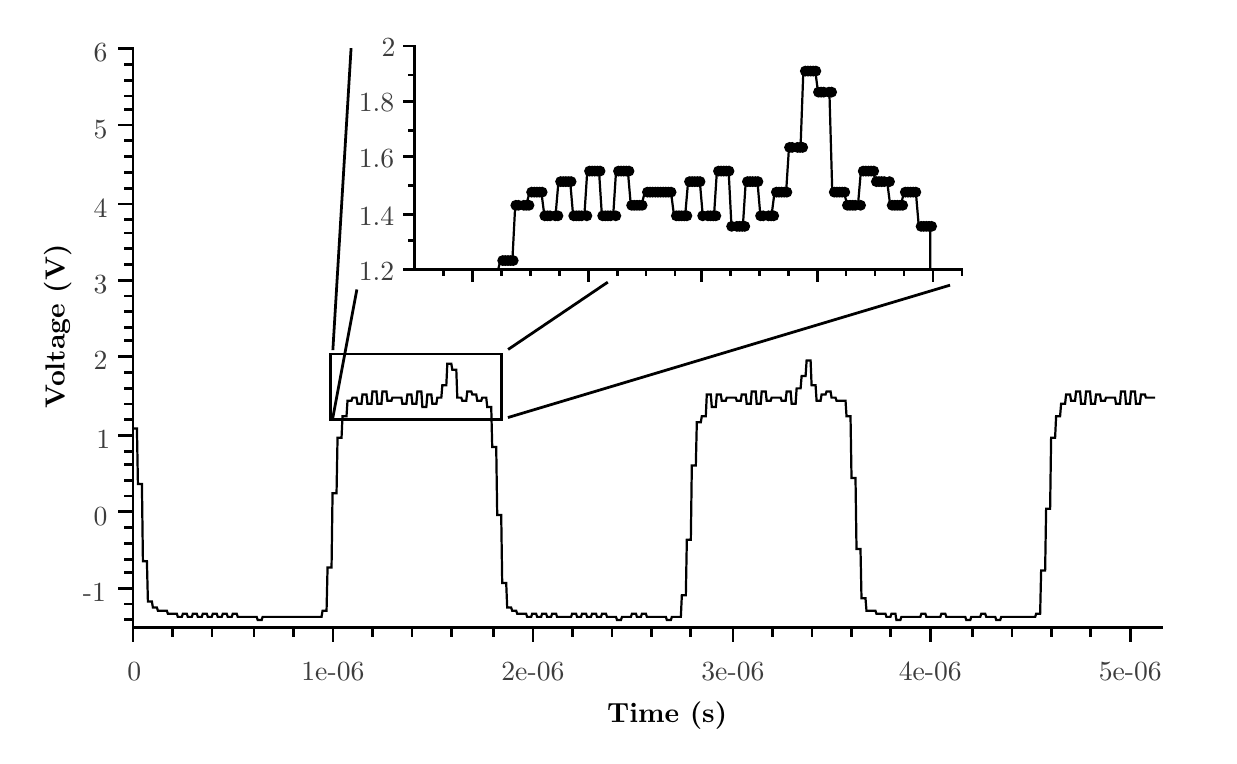
\begin{tikzpicture}{0pt}{0pt}{449pt}{269pt}
	\clip(0pt,269pt) -- (426.964pt,269pt) -- (426.964pt,13.2022pt) -- (0pt,13.2022pt) -- (0pt,269pt);
\begin{scope}
	\clip(139.785pt,262.344pt) -- (337.577pt,262.344pt) -- (337.577pt,181.515pt) -- (139.785pt,181.515pt) -- (139.785pt,262.344pt);
	\color[gray]{0}
	\draw[line width=0.8pt, line join=miter, line cap=rect](169.975pt,181.515pt) -- (171.016pt,185.557pt) -- (172.057pt,185.557pt) -- (173.098pt,185.557pt) -- (174.139pt,185.557pt) -- (175.18pt,185.557pt) -- (176.221pt,205.764pt) -- (177.262pt,205.764pt) -- (178.303pt,205.764pt) -- (179.344pt,205.764pt) -- (180.385pt,205.764pt) -- (181.426pt,209.805pt) -- (182.467pt,209.805pt) -- (183.508pt,209.805pt) -- (184.549pt,209.805pt) -- (185.59pt,209.805pt) -- (186.631pt,201.722pt) -- (187.672pt,201.722pt) -- (188.713pt,201.722pt) -- (189.754pt,201.722pt) -- (190.795pt,201.722pt) -- (191.836pt,213.847pt) -- (192.877pt,213.847pt) -- (193.918pt,213.847pt) -- (194.959pt,213.847pt) -- (196pt,213.847pt) -- (197.041pt,201.722pt) -- (198.082pt,201.722pt) -- (199.123pt,201.722pt) -- (200.164pt,201.722pt) -- (201.205pt,201.722pt) -- (202.246pt,217.888pt) -- (203.287pt,217.888pt) -- (204.328pt,217.888pt) -- (205.369pt,217.888pt) -- (206.41pt,217.888pt) -- (207.451pt,201.722pt) -- (208.492pt,201.722pt) -- (209.533pt,201.722pt) -- (210.574pt,201.722pt) -- (211.615pt,201.722pt) -- (212.656pt,217.888pt) -- (213.697pt,217.888pt) -- (214.738pt,217.888pt) -- (215.779pt,217.888pt) -- (216.82pt,217.888pt) -- (217.861pt,205.764pt) -- (218.902pt,205.764pt) -- (219.943pt,205.764pt) -- (220.984pt,205.764pt) -- (222.025pt,205.764pt) -- (223.066pt,209.805pt) -- (224.107pt,209.805pt) -- (225.148pt,209.805pt) -- (226.189pt,209.805pt) -- (227.23pt,209.805pt) -- (228.271pt,209.805pt) -- (229.312pt,209.805pt) -- (230.353pt,209.805pt) -- (231.394pt,209.805pt) -- (232.435pt,209.805pt) -- (233.476pt,201.722pt) -- (234.517pt,201.722pt) -- (235.558pt,201.722pt) -- (236.599pt,201.722pt) -- (237.64pt,201.722pt) -- (238.681pt,213.847pt) -- (239.722pt,213.847pt) -- (240.763pt,213.847pt) -- (241.804pt,213.847pt) -- (242.845pt,213.847pt) -- (243.886pt,201.722pt) -- (244.927pt,201.722pt) -- (245.968pt,201.722pt) -- (247.009pt,201.722pt) -- (248.05pt,201.722pt) -- (249.091pt,217.888pt) -- (250.132pt,217.888pt) -- (251.173pt,217.888pt) -- (252.214pt,217.888pt) -- (253.255pt,217.888pt) -- (254.296pt,197.681pt) -- (255.337pt,197.681pt) -- (256.378pt,197.681pt) -- (257.419pt,197.681pt) -- (258.46pt,197.681pt) -- (259.501pt,213.847pt) -- (260.542pt,213.847pt) -- (261.583pt,213.847pt) -- (262.624pt,213.847pt) -- (263.665pt,213.847pt) -- (264.706pt,201.722pt) -- (265.747pt,201.722pt) -- (266.788pt,201.722pt) -- (267.829pt,201.722pt) -- (268.87pt,201.722pt) -- (269.911pt,209.805pt) -- (270.952pt,209.805pt) -- (271.993pt,209.805pt) -- (273.034pt,209.805pt) -- (274.075pt,209.805pt) -- (275.116pt,225.971pt) -- (276.157pt,225.971pt) -- (277.198pt,225.971pt) -- (278.24pt,225.971pt) -- (279.281pt,225.971pt) -- (280.322pt,254.261pt) -- (281.363pt,254.261pt) -- (282.404pt,254.261pt) -- (283.445pt,254.261pt) -- (284.486pt,254.261pt) -- (285.527pt,246.178pt) -- (286.568pt,246.178pt) -- (287.609pt,246.178pt) -- (288.65pt,246.178pt) -- (289.691pt,246.178pt) -- (290.732pt,209.805pt) -- (291.773pt,209.805pt) -- (292.814pt,209.805pt) -- (293.855pt,209.805pt) -- (294.896pt,209.805pt) -- (295.937pt,205.764pt) -- (296.978pt,205.764pt) -- (298.019pt,205.764pt) -- (299.06pt,205.764pt) -- (300.101pt,205.764pt) -- (301.142pt,217.888pt) -- (302.183pt,217.888pt) -- (303.224pt,217.888pt) -- (304.265pt,217.888pt) -- (305.306pt,217.888pt) -- (306.347pt,213.847pt) -- (307.388pt,213.847pt) -- (308.429pt,213.847pt) -- (309.47pt,213.847pt) -- (310.511pt,213.847pt) -- (311.552pt,205.764pt) -- (312.593pt,205.764pt) -- (313.634pt,205.764pt) -- (314.675pt,205.764pt) -- (315.716pt,205.764pt) -- (316.757pt,209.805pt) -- (317.798pt,209.805pt) -- (318.839pt,209.805pt) -- (319.88pt,209.805pt) -- (320.921pt,209.805pt) -- (321.962pt,197.681pt) -- (323.003pt,197.681pt) -- (324.044pt,197.681pt) -- (325.085pt,197.681pt) -- (326.126pt,197.681pt) -- (326.126pt,181.515pt);
	\color[gray]{0}
	\fill(171.641pt,184.843pt) ellipse (1.42638pt and 1.42638pt);
	\draw[line width=1pt, line join=miter, line cap=rect](171.641pt,184.843pt) ellipse (1.42638pt and 1.42638pt);
	\fill(172.592pt,184.843pt) ellipse (1.42638pt and 1.42638pt);
	\draw[line width=1pt, line join=miter, line cap=rect](172.592pt,184.843pt) ellipse (1.42638pt and 1.42638pt);
	\fill(173.543pt,184.843pt) ellipse (1.42638pt and 1.42638pt);
	\draw[line width=1pt, line join=miter, line cap=rect](173.543pt,184.843pt) ellipse (1.42638pt and 1.42638pt);
	\fill(174.494pt,184.843pt) ellipse (1.42638pt and 1.42638pt);
	\draw[line width=1pt, line join=miter, line cap=rect](174.494pt,184.843pt) ellipse (1.42638pt and 1.42638pt);
	\fill(175.445pt,184.843pt) ellipse (1.42638pt and 1.42638pt);
	\draw[line width=1pt, line join=miter, line cap=rect](175.445pt,184.843pt) ellipse (1.42638pt and 1.42638pt);
	\fill(176.396pt,204.813pt) ellipse (1.42638pt and 1.42638pt);
	\draw[line width=1pt, line join=miter, line cap=rect](176.396pt,204.813pt) ellipse (1.42638pt and 1.42638pt);
	\fill(177.347pt,204.813pt) ellipse (1.42638pt and 1.42638pt);
	\draw[line width=1pt, line join=miter, line cap=rect](177.347pt,204.813pt) ellipse (1.42638pt and 1.42638pt);
	\fill(179.249pt,204.813pt) ellipse (1.42638pt and 1.42638pt);
	\draw[line width=1pt, line join=miter, line cap=rect](179.249pt,204.813pt) ellipse (1.42638pt and 1.42638pt);
	\fill(180.2pt,204.813pt) ellipse (1.42638pt and 1.42638pt);
	\draw[line width=1pt, line join=miter, line cap=rect](180.2pt,204.813pt) ellipse (1.42638pt and 1.42638pt);
	\fill(181.15pt,204.813pt) ellipse (1.42638pt and 1.42638pt);
	\draw[line width=1pt, line join=miter, line cap=rect](181.15pt,204.813pt) ellipse (1.42638pt and 1.42638pt);
	\fill(182.101pt,209.567pt) ellipse (1.42638pt and 1.42638pt);
	\draw[line width=1pt, line join=miter, line cap=rect](182.101pt,209.567pt) ellipse (1.42638pt and 1.42638pt);
	\fill(183.052pt,209.567pt) ellipse (1.42638pt and 1.42638pt);
	\draw[line width=1pt, line join=miter, line cap=rect](183.052pt,209.567pt) ellipse (1.42638pt and 1.42638pt);
	\fill(184.003pt,209.567pt) ellipse (1.42638pt and 1.42638pt);
	\draw[line width=1pt, line join=miter, line cap=rect](184.003pt,209.567pt) ellipse (1.42638pt and 1.42638pt);
	\fill(184.954pt,209.567pt) ellipse (1.42638pt and 1.42638pt);
	\draw[line width=1pt, line join=miter, line cap=rect](184.954pt,209.567pt) ellipse (1.42638pt and 1.42638pt);
	\fill(185.905pt,209.567pt) ellipse (1.42638pt and 1.42638pt);
	\draw[line width=1pt, line join=miter, line cap=rect](185.905pt,209.567pt) ellipse (1.42638pt and 1.42638pt);
	\fill(186.856pt,201.009pt) ellipse (1.42638pt and 1.42638pt);
	\draw[line width=1pt, line join=miter, line cap=rect](186.856pt,201.009pt) ellipse (1.42638pt and 1.42638pt);
	\fill(187.807pt,201.009pt) ellipse (1.42638pt and 1.42638pt);
	\draw[line width=1pt, line join=miter, line cap=rect](187.807pt,201.009pt) ellipse (1.42638pt and 1.42638pt);
	\fill(188.758pt,201.009pt) ellipse (1.42638pt and 1.42638pt);
	\draw[line width=1pt, line join=miter, line cap=rect](188.758pt,201.009pt) ellipse (1.42638pt and 1.42638pt);
	\fill(190.66pt,201.009pt) ellipse (1.42638pt and 1.42638pt);
	\draw[line width=1pt, line join=miter, line cap=rect](190.66pt,201.009pt) ellipse (1.42638pt and 1.42638pt);
	\fill(191.611pt,201.009pt) ellipse (1.42638pt and 1.42638pt);
	\draw[line width=1pt, line join=miter, line cap=rect](191.611pt,201.009pt) ellipse (1.42638pt and 1.42638pt);
	\fill(192.562pt,213.371pt) ellipse (1.42638pt and 1.42638pt);
	\draw[line width=1pt, line join=miter, line cap=rect](192.562pt,213.371pt) ellipse (1.42638pt and 1.42638pt);
	\fill(193.512pt,213.371pt) ellipse (1.42638pt and 1.42638pt);
	\draw[line width=1pt, line join=miter, line cap=rect](193.512pt,213.371pt) ellipse (1.42638pt and 1.42638pt);
	\fill(194.463pt,213.371pt) ellipse (1.42638pt and 1.42638pt);
	\draw[line width=1pt, line join=miter, line cap=rect](194.463pt,213.371pt) ellipse (1.42638pt and 1.42638pt);
	\fill(195.414pt,213.371pt) ellipse (1.42638pt and 1.42638pt);
	\draw[line width=1pt, line join=miter, line cap=rect](195.414pt,213.371pt) ellipse (1.42638pt and 1.42638pt);
	\fill(196.365pt,213.371pt) ellipse (1.42638pt and 1.42638pt);
	\draw[line width=1pt, line join=miter, line cap=rect](196.365pt,213.371pt) ellipse (1.42638pt and 1.42638pt);
	\fill(197.316pt,201.009pt) ellipse (1.42638pt and 1.42638pt);
	\draw[line width=1pt, line join=miter, line cap=rect](197.316pt,201.009pt) ellipse (1.42638pt and 1.42638pt);
	\fill(198.267pt,201.009pt) ellipse (1.42638pt and 1.42638pt);
	\draw[line width=1pt, line join=miter, line cap=rect](198.267pt,201.009pt) ellipse (1.42638pt and 1.42638pt);
	\fill(199.218pt,201.009pt) ellipse (1.42638pt and 1.42638pt);
	\draw[line width=1pt, line join=miter, line cap=rect](199.218pt,201.009pt) ellipse (1.42638pt and 1.42638pt);
	\fill(200.169pt,201.009pt) ellipse (1.42638pt and 1.42638pt);
	\draw[line width=1pt, line join=miter, line cap=rect](200.169pt,201.009pt) ellipse (1.42638pt and 1.42638pt);
	\fill(202.071pt,201.009pt) ellipse (1.42638pt and 1.42638pt);
	\draw[line width=1pt, line join=miter, line cap=rect](202.071pt,201.009pt) ellipse (1.42638pt and 1.42638pt);
	\fill(203.022pt,217.175pt) ellipse (1.42638pt and 1.42638pt);
	\draw[line width=1pt, line join=miter, line cap=rect](203.022pt,217.175pt) ellipse (1.42638pt and 1.42638pt);
	\fill(203.973pt,217.175pt) ellipse (1.42638pt and 1.42638pt);
	\draw[line width=1pt, line join=miter, line cap=rect](203.973pt,217.175pt) ellipse (1.42638pt and 1.42638pt);
	\fill(204.923pt,217.175pt) ellipse (1.42638pt and 1.42638pt);
	\draw[line width=1pt, line join=miter, line cap=rect](204.923pt,217.175pt) ellipse (1.42638pt and 1.42638pt);
	\fill(205.874pt,217.175pt) ellipse (1.42638pt and 1.42638pt);
	\draw[line width=1pt, line join=miter, line cap=rect](205.874pt,217.175pt) ellipse (1.42638pt and 1.42638pt);
	\fill(206.825pt,217.175pt) ellipse (1.42638pt and 1.42638pt);
	\draw[line width=1pt, line join=miter, line cap=rect](206.825pt,217.175pt) ellipse (1.42638pt and 1.42638pt);
	\fill(207.776pt,201.009pt) ellipse (1.42638pt and 1.42638pt);
	\draw[line width=1pt, line join=miter, line cap=rect](207.776pt,201.009pt) ellipse (1.42638pt and 1.42638pt);
	\fill(208.727pt,201.009pt) ellipse (1.42638pt and 1.42638pt);
	\draw[line width=1pt, line join=miter, line cap=rect](208.727pt,201.009pt) ellipse (1.42638pt and 1.42638pt);
	\fill(209.678pt,201.009pt) ellipse (1.42638pt and 1.42638pt);
	\draw[line width=1pt, line join=miter, line cap=rect](209.678pt,201.009pt) ellipse (1.42638pt and 1.42638pt);
	\fill(210.629pt,201.009pt) ellipse (1.42638pt and 1.42638pt);
	\draw[line width=1pt, line join=miter, line cap=rect](210.629pt,201.009pt) ellipse (1.42638pt and 1.42638pt);
	\fill(212.531pt,201.009pt) ellipse (1.42638pt and 1.42638pt);
	\draw[line width=1pt, line join=miter, line cap=rect](212.531pt,201.009pt) ellipse (1.42638pt and 1.42638pt);
	\fill(213.482pt,217.175pt) ellipse (1.42638pt and 1.42638pt);
	\draw[line width=1pt, line join=miter, line cap=rect](213.482pt,217.175pt) ellipse (1.42638pt and 1.42638pt);
	\fill(214.433pt,217.175pt) ellipse (1.42638pt and 1.42638pt);
	\draw[line width=1pt, line join=miter, line cap=rect](214.433pt,217.175pt) ellipse (1.42638pt and 1.42638pt);
	\fill(215.384pt,217.175pt) ellipse (1.42638pt and 1.42638pt);
	\draw[line width=1pt, line join=miter, line cap=rect](215.384pt,217.175pt) ellipse (1.42638pt and 1.42638pt);
	\fill(216.335pt,217.175pt) ellipse (1.42638pt and 1.42638pt);
	\draw[line width=1pt, line join=miter, line cap=rect](216.335pt,217.175pt) ellipse (1.42638pt and 1.42638pt);
	\fill(217.285pt,217.175pt) ellipse (1.42638pt and 1.42638pt);
	\draw[line width=1pt, line join=miter, line cap=rect](217.285pt,217.175pt) ellipse (1.42638pt and 1.42638pt);
	\fill(218.236pt,204.813pt) ellipse (1.42638pt and 1.42638pt);
	\draw[line width=1pt, line join=miter, line cap=rect](218.236pt,204.813pt) ellipse (1.42638pt and 1.42638pt);
	\fill(219.187pt,204.813pt) ellipse (1.42638pt and 1.42638pt);
	\draw[line width=1pt, line join=miter, line cap=rect](219.187pt,204.813pt) ellipse (1.42638pt and 1.42638pt);
	\fill(220.138pt,204.813pt) ellipse (1.42638pt and 1.42638pt);
	\draw[line width=1pt, line join=miter, line cap=rect](220.138pt,204.813pt) ellipse (1.42638pt and 1.42638pt);
	\fill(221.089pt,204.813pt) ellipse (1.42638pt and 1.42638pt);
	\draw[line width=1pt, line join=miter, line cap=rect](221.089pt,204.813pt) ellipse (1.42638pt and 1.42638pt);
	\fill(222.04pt,204.813pt) ellipse (1.42638pt and 1.42638pt);
	\draw[line width=1pt, line join=miter, line cap=rect](222.04pt,204.813pt) ellipse (1.42638pt and 1.42638pt);
	\fill(223.942pt,209.567pt) ellipse (1.42638pt and 1.42638pt);
	\draw[line width=1pt, line join=miter, line cap=rect](223.942pt,209.567pt) ellipse (1.42638pt and 1.42638pt);
	\fill(224.893pt,209.567pt) ellipse (1.42638pt and 1.42638pt);
	\draw[line width=1pt, line join=miter, line cap=rect](224.893pt,209.567pt) ellipse (1.42638pt and 1.42638pt);
	\fill(225.844pt,209.567pt) ellipse (1.42638pt and 1.42638pt);
	\draw[line width=1pt, line join=miter, line cap=rect](225.844pt,209.567pt) ellipse (1.42638pt and 1.42638pt);
	\fill(226.795pt,209.567pt) ellipse (1.42638pt and 1.42638pt);
	\draw[line width=1pt, line join=miter, line cap=rect](226.795pt,209.567pt) ellipse (1.42638pt and 1.42638pt);
	\fill(227.746pt,209.567pt) ellipse (1.42638pt and 1.42638pt);
	\draw[line width=1pt, line join=miter, line cap=rect](227.746pt,209.567pt) ellipse (1.42638pt and 1.42638pt);
	\fill(228.697pt,209.567pt) ellipse (1.42638pt and 1.42638pt);
	\draw[line width=1pt, line join=miter, line cap=rect](228.697pt,209.567pt) ellipse (1.42638pt and 1.42638pt);
	\fill(229.647pt,209.567pt) ellipse (1.42638pt and 1.42638pt);
	\draw[line width=1pt, line join=miter, line cap=rect](229.647pt,209.567pt) ellipse (1.42638pt and 1.42638pt);
	\fill(230.598pt,209.567pt) ellipse (1.42638pt and 1.42638pt);
	\draw[line width=1pt, line join=miter, line cap=rect](230.598pt,209.567pt) ellipse (1.42638pt and 1.42638pt);
	\fill(231.549pt,209.567pt) ellipse (1.42638pt and 1.42638pt);
	\draw[line width=1pt, line join=miter, line cap=rect](231.549pt,209.567pt) ellipse (1.42638pt and 1.42638pt);
	\fill(232.5pt,209.567pt) ellipse (1.42638pt and 1.42638pt);
	\draw[line width=1pt, line join=miter, line cap=rect](232.5pt,209.567pt) ellipse (1.42638pt and 1.42638pt);
	\fill(234.402pt,201.009pt) ellipse (1.42638pt and 1.42638pt);
	\draw[line width=1pt, line join=miter, line cap=rect](234.402pt,201.009pt) ellipse (1.42638pt and 1.42638pt);
	\fill(235.353pt,201.009pt) ellipse (1.42638pt and 1.42638pt);
	\draw[line width=1pt, line join=miter, line cap=rect](235.353pt,201.009pt) ellipse (1.42638pt and 1.42638pt);
	\fill(236.304pt,201.009pt) ellipse (1.42638pt and 1.42638pt);
	\draw[line width=1pt, line join=miter, line cap=rect](236.304pt,201.009pt) ellipse (1.42638pt and 1.42638pt);
	\fill(237.255pt,201.009pt) ellipse (1.42638pt and 1.42638pt);
	\draw[line width=1pt, line join=miter, line cap=rect](237.255pt,201.009pt) ellipse (1.42638pt and 1.42638pt);
	\fill(238.206pt,201.009pt) ellipse (1.42638pt and 1.42638pt);
	\draw[line width=1pt, line join=miter, line cap=rect](238.206pt,201.009pt) ellipse (1.42638pt and 1.42638pt);
	\fill(239.157pt,213.371pt) ellipse (1.42638pt and 1.42638pt);
	\draw[line width=1pt, line join=miter, line cap=rect](239.157pt,213.371pt) ellipse (1.42638pt and 1.42638pt);
	\fill(240.108pt,213.371pt) ellipse (1.42638pt and 1.42638pt);
	\draw[line width=1pt, line join=miter, line cap=rect](240.108pt,213.371pt) ellipse (1.42638pt and 1.42638pt);
	\fill(241.058pt,213.371pt) ellipse (1.42638pt and 1.42638pt);
	\draw[line width=1pt, line join=miter, line cap=rect](241.058pt,213.371pt) ellipse (1.42638pt and 1.42638pt);
	\fill(242.009pt,213.371pt) ellipse (1.42638pt and 1.42638pt);
	\draw[line width=1pt, line join=miter, line cap=rect](242.009pt,213.371pt) ellipse (1.42638pt and 1.42638pt);
	\fill(242.96pt,213.371pt) ellipse (1.42638pt and 1.42638pt);
	\draw[line width=1pt, line join=miter, line cap=rect](242.96pt,213.371pt) ellipse (1.42638pt and 1.42638pt);
	\fill(243.911pt,201.009pt) ellipse (1.42638pt and 1.42638pt);
	\draw[line width=1pt, line join=miter, line cap=rect](243.911pt,201.009pt) ellipse (1.42638pt and 1.42638pt);
	\fill(245.813pt,201.009pt) ellipse (1.42638pt and 1.42638pt);
	\draw[line width=1pt, line join=miter, line cap=rect](245.813pt,201.009pt) ellipse (1.42638pt and 1.42638pt);
	\fill(246.764pt,201.009pt) ellipse (1.42638pt and 1.42638pt);
	\draw[line width=1pt, line join=miter, line cap=rect](246.764pt,201.009pt) ellipse (1.42638pt and 1.42638pt);
	\fill(247.715pt,201.009pt) ellipse (1.42638pt and 1.42638pt);
	\draw[line width=1pt, line join=miter, line cap=rect](247.715pt,201.009pt) ellipse (1.42638pt and 1.42638pt);
	\fill(248.666pt,201.009pt) ellipse (1.42638pt and 1.42638pt);
	\draw[line width=1pt, line join=miter, line cap=rect](248.666pt,201.009pt) ellipse (1.42638pt and 1.42638pt);
	\fill(249.617pt,217.175pt) ellipse (1.42638pt and 1.42638pt);
	\draw[line width=1pt, line join=miter, line cap=rect](249.617pt,217.175pt) ellipse (1.42638pt and 1.42638pt);
	\fill(250.568pt,217.175pt) ellipse (1.42638pt and 1.42638pt);
	\draw[line width=1pt, line join=miter, line cap=rect](250.568pt,217.175pt) ellipse (1.42638pt and 1.42638pt);
	\fill(251.519pt,217.175pt) ellipse (1.42638pt and 1.42638pt);
	\draw[line width=1pt, line join=miter, line cap=rect](251.519pt,217.175pt) ellipse (1.42638pt and 1.42638pt);
	\fill(252.47pt,217.175pt) ellipse (1.42638pt and 1.42638pt);
	\draw[line width=1pt, line join=miter, line cap=rect](252.47pt,217.175pt) ellipse (1.42638pt and 1.42638pt);
	\fill(253.42pt,217.175pt) ellipse (1.42638pt and 1.42638pt);
	\draw[line width=1pt, line join=miter, line cap=rect](253.42pt,217.175pt) ellipse (1.42638pt and 1.42638pt);
	\fill(254.371pt,197.205pt) ellipse (1.42638pt and 1.42638pt);
	\draw[line width=1pt, line join=miter, line cap=rect](254.371pt,197.205pt) ellipse (1.42638pt and 1.42638pt);
	\fill(256.273pt,197.205pt) ellipse (1.42638pt and 1.42638pt);
	\draw[line width=1pt, line join=miter, line cap=rect](256.273pt,197.205pt) ellipse (1.42638pt and 1.42638pt);
	\fill(257.224pt,197.205pt) ellipse (1.42638pt and 1.42638pt);
	\draw[line width=1pt, line join=miter, line cap=rect](257.224pt,197.205pt) ellipse (1.42638pt and 1.42638pt);
	\fill(258.175pt,197.205pt) ellipse (1.42638pt and 1.42638pt);
	\draw[line width=1pt, line join=miter, line cap=rect](258.175pt,197.205pt) ellipse (1.42638pt and 1.42638pt);
	\fill(259.126pt,197.205pt) ellipse (1.42638pt and 1.42638pt);
	\draw[line width=1pt, line join=miter, line cap=rect](259.126pt,197.205pt) ellipse (1.42638pt and 1.42638pt);
	\fill(260.077pt,213.371pt) ellipse (1.42638pt and 1.42638pt);
	\draw[line width=1pt, line join=miter, line cap=rect](260.077pt,213.371pt) ellipse (1.42638pt and 1.42638pt);
	\fill(261.028pt,213.371pt) ellipse (1.42638pt and 1.42638pt);
	\draw[line width=1pt, line join=miter, line cap=rect](261.028pt,213.371pt) ellipse (1.42638pt and 1.42638pt);
	\fill(261.979pt,213.371pt) ellipse (1.42638pt and 1.42638pt);
	\draw[line width=1pt, line join=miter, line cap=rect](261.979pt,213.371pt) ellipse (1.42638pt and 1.42638pt);
	\fill(262.93pt,213.371pt) ellipse (1.42638pt and 1.42638pt);
	\draw[line width=1pt, line join=miter, line cap=rect](262.93pt,213.371pt) ellipse (1.42638pt and 1.42638pt);
	\fill(263.881pt,213.371pt) ellipse (1.42638pt and 1.42638pt);
	\draw[line width=1pt, line join=miter, line cap=rect](263.881pt,213.371pt) ellipse (1.42638pt and 1.42638pt);
	\fill(264.832pt,201.009pt) ellipse (1.42638pt and 1.42638pt);
	\draw[line width=1pt, line join=miter, line cap=rect](264.832pt,201.009pt) ellipse (1.42638pt and 1.42638pt);
	\fill(265.782pt,201.009pt) ellipse (1.42638pt and 1.42638pt);
	\draw[line width=1pt, line join=miter, line cap=rect](265.782pt,201.009pt) ellipse (1.42638pt and 1.42638pt);
	\fill(267.684pt,201.009pt) ellipse (1.42638pt and 1.42638pt);
	\draw[line width=1pt, line join=miter, line cap=rect](267.684pt,201.009pt) ellipse (1.42638pt and 1.42638pt);
	\fill(268.635pt,201.009pt) ellipse (1.42638pt and 1.42638pt);
	\draw[line width=1pt, line join=miter, line cap=rect](268.635pt,201.009pt) ellipse (1.42638pt and 1.42638pt);
	\fill(269.586pt,201.009pt) ellipse (1.42638pt and 1.42638pt);
	\draw[line width=1pt, line join=miter, line cap=rect](269.586pt,201.009pt) ellipse (1.42638pt and 1.42638pt);
	\fill(270.537pt,209.567pt) ellipse (1.42638pt and 1.42638pt);
	\draw[line width=1pt, line join=miter, line cap=rect](270.537pt,209.567pt) ellipse (1.42638pt and 1.42638pt);
	\fill(271.488pt,209.567pt) ellipse (1.42638pt and 1.42638pt);
	\draw[line width=1pt, line join=miter, line cap=rect](271.488pt,209.567pt) ellipse (1.42638pt and 1.42638pt);
	\fill(272.439pt,209.567pt) ellipse (1.42638pt and 1.42638pt);
	\draw[line width=1pt, line join=miter, line cap=rect](272.439pt,209.567pt) ellipse (1.42638pt and 1.42638pt);
	\fill(273.39pt,209.567pt) ellipse (1.42638pt and 1.42638pt);
	\draw[line width=1pt, line join=miter, line cap=rect](273.39pt,209.567pt) ellipse (1.42638pt and 1.42638pt);
	\fill(274.341pt,209.567pt) ellipse (1.42638pt and 1.42638pt);
	\draw[line width=1pt, line join=miter, line cap=rect](274.341pt,209.567pt) ellipse (1.42638pt and 1.42638pt);
	\fill(275.292pt,225.733pt) ellipse (1.42638pt and 1.42638pt);
	\draw[line width=1pt, line join=miter, line cap=rect](275.292pt,225.733pt) ellipse (1.42638pt and 1.42638pt);
	\fill(276.243pt,225.733pt) ellipse (1.42638pt and 1.42638pt);
	\draw[line width=1pt, line join=miter, line cap=rect](276.243pt,225.733pt) ellipse (1.42638pt and 1.42638pt);
	\fill(278.144pt,225.733pt) ellipse (1.42638pt and 1.42638pt);
	\draw[line width=1pt, line join=miter, line cap=rect](278.144pt,225.733pt) ellipse (1.42638pt and 1.42638pt);
	\fill(279.095pt,225.733pt) ellipse (1.42638pt and 1.42638pt);
	\draw[line width=1pt, line join=miter, line cap=rect](279.095pt,225.733pt) ellipse (1.42638pt and 1.42638pt);
	\fill(280.046pt,225.733pt) ellipse (1.42638pt and 1.42638pt);
	\draw[line width=1pt, line join=miter, line cap=rect](280.046pt,225.733pt) ellipse (1.42638pt and 1.42638pt);
	\fill(280.997pt,253.31pt) ellipse (1.42638pt and 1.42638pt);
	\draw[line width=1pt, line join=miter, line cap=rect](280.997pt,253.31pt) ellipse (1.42638pt and 1.42638pt);
	\fill(281.948pt,253.31pt) ellipse (1.42638pt and 1.42638pt);
	\draw[line width=1pt, line join=miter, line cap=rect](281.948pt,253.31pt) ellipse (1.42638pt and 1.42638pt);
	\fill(282.899pt,253.31pt) ellipse (1.42638pt and 1.42638pt);
	\draw[line width=1pt, line join=miter, line cap=rect](282.899pt,253.31pt) ellipse (1.42638pt and 1.42638pt);
	\fill(283.85pt,253.31pt) ellipse (1.42638pt and 1.42638pt);
	\draw[line width=1pt, line join=miter, line cap=rect](283.85pt,253.31pt) ellipse (1.42638pt and 1.42638pt);
	\fill(284.801pt,253.31pt) ellipse (1.42638pt and 1.42638pt);
	\draw[line width=1pt, line join=miter, line cap=rect](284.801pt,253.31pt) ellipse (1.42638pt and 1.42638pt);
	\fill(285.752pt,245.702pt) ellipse (1.42638pt and 1.42638pt);
	\draw[line width=1pt, line join=miter, line cap=rect](285.752pt,245.702pt) ellipse (1.42638pt and 1.42638pt);
	\fill(286.703pt,245.702pt) ellipse (1.42638pt and 1.42638pt);
	\draw[line width=1pt, line join=miter, line cap=rect](286.703pt,245.702pt) ellipse (1.42638pt and 1.42638pt);
	\fill(287.654pt,245.702pt) ellipse (1.42638pt and 1.42638pt);
	\draw[line width=1pt, line join=miter, line cap=rect](287.654pt,245.702pt) ellipse (1.42638pt and 1.42638pt);
	\fill(289.555pt,245.702pt) ellipse (1.42638pt and 1.42638pt);
	\draw[line width=1pt, line join=miter, line cap=rect](289.555pt,245.702pt) ellipse (1.42638pt and 1.42638pt);
	\fill(290.506pt,245.702pt) ellipse (1.42638pt and 1.42638pt);
	\draw[line width=1pt, line join=miter, line cap=rect](290.506pt,245.702pt) ellipse (1.42638pt and 1.42638pt);
	\fill(291.457pt,209.567pt) ellipse (1.42638pt and 1.42638pt);
	\draw[line width=1pt, line join=miter, line cap=rect](291.457pt,209.567pt) ellipse (1.42638pt and 1.42638pt);
	\fill(292.408pt,209.567pt) ellipse (1.42638pt and 1.42638pt);
	\draw[line width=1pt, line join=miter, line cap=rect](292.408pt,209.567pt) ellipse (1.42638pt and 1.42638pt);
	\fill(293.359pt,209.567pt) ellipse (1.42638pt and 1.42638pt);
	\draw[line width=1pt, line join=miter, line cap=rect](293.359pt,209.567pt) ellipse (1.42638pt and 1.42638pt);
	\fill(294.31pt,209.567pt) ellipse (1.42638pt and 1.42638pt);
	\draw[line width=1pt, line join=miter, line cap=rect](294.31pt,209.567pt) ellipse (1.42638pt and 1.42638pt);
	\fill(295.261pt,209.567pt) ellipse (1.42638pt and 1.42638pt);
	\draw[line width=1pt, line join=miter, line cap=rect](295.261pt,209.567pt) ellipse (1.42638pt and 1.42638pt);
	\fill(296.212pt,204.813pt) ellipse (1.42638pt and 1.42638pt);
	\draw[line width=1pt, line join=miter, line cap=rect](296.212pt,204.813pt) ellipse (1.42638pt and 1.42638pt);
	\fill(297.163pt,204.813pt) ellipse (1.42638pt and 1.42638pt);
	\draw[line width=1pt, line join=miter, line cap=rect](297.163pt,204.813pt) ellipse (1.42638pt and 1.42638pt);
	\fill(298.114pt,204.813pt) ellipse (1.42638pt and 1.42638pt);
	\draw[line width=1pt, line join=miter, line cap=rect](298.114pt,204.813pt) ellipse (1.42638pt and 1.42638pt);
	\fill(299.065pt,204.813pt) ellipse (1.42638pt and 1.42638pt);
	\draw[line width=1pt, line join=miter, line cap=rect](299.065pt,204.813pt) ellipse (1.42638pt and 1.42638pt);
	\fill(300.967pt,204.813pt) ellipse (1.42638pt and 1.42638pt);
	\draw[line width=1pt, line join=miter, line cap=rect](300.967pt,204.813pt) ellipse (1.42638pt and 1.42638pt);
	\fill(301.917pt,217.175pt) ellipse (1.42638pt and 1.42638pt);
	\draw[line width=1pt, line join=miter, line cap=rect](301.917pt,217.175pt) ellipse (1.42638pt and 1.42638pt);
	\fill(302.868pt,217.175pt) ellipse (1.42638pt and 1.42638pt);
	\draw[line width=1pt, line join=miter, line cap=rect](302.868pt,217.175pt) ellipse (1.42638pt and 1.42638pt);
	\fill(303.819pt,217.175pt) ellipse (1.42638pt and 1.42638pt);
	\draw[line width=1pt, line join=miter, line cap=rect](303.819pt,217.175pt) ellipse (1.42638pt and 1.42638pt);
	\fill(304.77pt,217.175pt) ellipse (1.42638pt and 1.42638pt);
	\draw[line width=1pt, line join=miter, line cap=rect](304.77pt,217.175pt) ellipse (1.42638pt and 1.42638pt);
	\fill(305.721pt,217.175pt) ellipse (1.42638pt and 1.42638pt);
	\draw[line width=1pt, line join=miter, line cap=rect](305.721pt,217.175pt) ellipse (1.42638pt and 1.42638pt);
	\fill(306.672pt,213.371pt) ellipse (1.42638pt and 1.42638pt);
	\draw[line width=1pt, line join=miter, line cap=rect](306.672pt,213.371pt) ellipse (1.42638pt and 1.42638pt);
	\fill(307.623pt,213.371pt) ellipse (1.42638pt and 1.42638pt);
	\draw[line width=1pt, line join=miter, line cap=rect](307.623pt,213.371pt) ellipse (1.42638pt and 1.42638pt);
	\fill(308.574pt,213.371pt) ellipse (1.42638pt and 1.42638pt);
	\draw[line width=1pt, line join=miter, line cap=rect](308.574pt,213.371pt) ellipse (1.42638pt and 1.42638pt);
	\fill(309.525pt,213.371pt) ellipse (1.42638pt and 1.42638pt);
	\draw[line width=1pt, line join=miter, line cap=rect](309.525pt,213.371pt) ellipse (1.42638pt and 1.42638pt);
	\fill(311.427pt,213.371pt) ellipse (1.42638pt and 1.42638pt);
	\draw[line width=1pt, line join=miter, line cap=rect](311.427pt,213.371pt) ellipse (1.42638pt and 1.42638pt);
	\fill(312.378pt,204.813pt) ellipse (1.42638pt and 1.42638pt);
	\draw[line width=1pt, line join=miter, line cap=rect](312.378pt,204.813pt) ellipse (1.42638pt and 1.42638pt);
	\fill(313.328pt,204.813pt) ellipse (1.42638pt and 1.42638pt);
	\draw[line width=1pt, line join=miter, line cap=rect](313.328pt,204.813pt) ellipse (1.42638pt and 1.42638pt);
	\fill(314.279pt,204.813pt) ellipse (1.42638pt and 1.42638pt);
	\draw[line width=1pt, line join=miter, line cap=rect](314.279pt,204.813pt) ellipse (1.42638pt and 1.42638pt);
	\fill(315.23pt,204.813pt) ellipse (1.42638pt and 1.42638pt);
	\draw[line width=1pt, line join=miter, line cap=rect](315.23pt,204.813pt) ellipse (1.42638pt and 1.42638pt);
	\fill(316.181pt,204.813pt) ellipse (1.42638pt and 1.42638pt);
	\draw[line width=1pt, line join=miter, line cap=rect](316.181pt,204.813pt) ellipse (1.42638pt and 1.42638pt);
	\fill(317.132pt,209.567pt) ellipse (1.42638pt and 1.42638pt);
	\draw[line width=1pt, line join=miter, line cap=rect](317.132pt,209.567pt) ellipse (1.42638pt and 1.42638pt);
	\fill(318.083pt,209.567pt) ellipse (1.42638pt and 1.42638pt);
	\draw[line width=1pt, line join=miter, line cap=rect](318.083pt,209.567pt) ellipse (1.42638pt and 1.42638pt);
	\fill(319.034pt,209.567pt) ellipse (1.42638pt and 1.42638pt);
	\draw[line width=1pt, line join=miter, line cap=rect](319.034pt,209.567pt) ellipse (1.42638pt and 1.42638pt);
	\fill(319.985pt,209.567pt) ellipse (1.42638pt and 1.42638pt);
	\draw[line width=1pt, line join=miter, line cap=rect](319.985pt,209.567pt) ellipse (1.42638pt and 1.42638pt);
	\fill(320.936pt,209.567pt) ellipse (1.42638pt and 1.42638pt);
	\draw[line width=1pt, line join=miter, line cap=rect](320.936pt,209.567pt) ellipse (1.42638pt and 1.42638pt);
	\fill(322.838pt,197.205pt) ellipse (1.42638pt and 1.42638pt);
	\draw[line width=1pt, line join=miter, line cap=rect](322.838pt,197.205pt) ellipse (1.42638pt and 1.42638pt);
	\fill(323.789pt,197.205pt) ellipse (1.42638pt and 1.42638pt);
	\draw[line width=1pt, line join=miter, line cap=rect](323.789pt,197.205pt) ellipse (1.42638pt and 1.42638pt);
	\fill(324.74pt,197.205pt) ellipse (1.42638pt and 1.42638pt);
	\draw[line width=1pt, line join=miter, line cap=rect](324.74pt,197.205pt) ellipse (1.42638pt and 1.42638pt);
	\fill(325.69pt,197.205pt) ellipse (1.42638pt and 1.42638pt);
	\draw[line width=1pt, line join=miter, line cap=rect](325.69pt,197.205pt) ellipse (1.42638pt and 1.42638pt);
	\fill(326.641pt,197.205pt) ellipse (1.42638pt and 1.42638pt);
	\draw[line width=1pt, line join=miter, line cap=rect](326.641pt,197.205pt) ellipse (1.42638pt and 1.42638pt);
\end{scope}
\begin{scope}
	\color[gray]{0.235294}
	\pgftext[center, base, at={\pgfpoint{126.049pt}{177.712pt}}]{1.2}
	\pgftext[center, base, at={\pgfpoint{126.049pt}{197.681pt}}]{1.4}
	\pgftext[center, base, at={\pgfpoint{126.049pt}{218.601pt}}]{1.6}
	\pgftext[center, base, at={\pgfpoint{126.049pt}{238.571pt}}]{1.8}
	\pgftext[center, base, at={\pgfpoint{130.373pt}{258.54pt}}]{2}
	\color[gray]{0}
	\draw[line width=1pt, line join=bevel, line cap=rect](139.785pt,191.975pt) -- (137.884pt,191.975pt);
	\draw[line width=1pt, line join=bevel, line cap=rect](139.785pt,211.945pt) -- (137.884pt,211.945pt);
	\draw[line width=1pt, line join=bevel, line cap=rect](139.785pt,231.914pt) -- (137.884pt,231.914pt);
	\draw[line width=1pt, line join=bevel, line cap=rect](139.785pt,251.883pt) -- (137.884pt,251.883pt);
	\draw[line width=1pt, line join=bevel, line cap=rect](139.785pt,181.515pt) -- (135.982pt,181.515pt);
	\draw[line width=1pt, line join=bevel, line cap=rect](139.785pt,201.485pt) -- (135.982pt,201.485pt);
	\draw[line width=1pt, line join=bevel, line cap=rect](139.785pt,222.405pt) -- (135.982pt,222.405pt);
	\draw[line width=1pt, line join=bevel, line cap=rect](139.785pt,242.374pt) -- (135.982pt,242.374pt);
	\draw[line width=1pt, line join=bevel, line cap=rect](139.785pt,262.344pt) -- (135.982pt,262.344pt);
	\draw[line width=1pt, line join=bevel, line cap=rect](139.785pt,262.344pt) -- (139.785pt,181.515pt);
	\draw[line width=1pt, line join=bevel, line cap=rect](150.246pt,181.515pt) -- (150.246pt,179.613pt);
	\draw[line width=1pt, line join=bevel, line cap=rect](171.166pt,181.515pt) -- (171.166pt,179.613pt);
	\draw[line width=1pt, line join=bevel, line cap=rect](192.086pt,181.515pt) -- (192.086pt,179.613pt);
	\draw[line width=1pt, line join=bevel, line cap=rect](213.006pt,181.515pt) -- (213.006pt,179.613pt);
	\draw[line width=1pt, line join=bevel, line cap=rect](233.927pt,181.515pt) -- (233.927pt,179.613pt);
	\draw[line width=1pt, line join=bevel, line cap=rect](253.896pt,181.515pt) -- (253.896pt,179.613pt);
	\draw[line width=1pt, line join=bevel, line cap=rect](274.816pt,181.515pt) -- (274.816pt,179.613pt);
	\draw[line width=1pt, line join=bevel, line cap=rect](295.736pt,181.515pt) -- (295.736pt,179.613pt);
	\draw[line width=1pt, line join=bevel, line cap=rect](316.657pt,181.515pt) -- (316.657pt,179.613pt);
	\draw[line width=1pt, line join=bevel, line cap=rect](337.577pt,181.515pt) -- (337.577pt,179.613pt);
	\draw[line width=1pt, line join=bevel, line cap=rect](181.626pt,181.515pt) -- (181.626pt,179.613pt);
	\draw[line width=1pt, line join=bevel, line cap=rect](223.466pt,181.515pt) -- (223.466pt,179.613pt);
	\draw[line width=1pt, line join=bevel, line cap=rect](264.356pt,181.515pt) -- (264.356pt,179.613pt);
	\draw[line width=1pt, line join=bevel, line cap=rect](306.197pt,181.515pt) -- (306.197pt,179.613pt);
	\draw[line width=1pt, line join=bevel, line cap=rect](160.706pt,181.515pt) -- (160.706pt,177.712pt);
	\draw[line width=1pt, line join=bevel, line cap=rect](202.546pt,181.515pt) -- (202.546pt,177.712pt);
	\draw[line width=1pt, line join=bevel, line cap=rect](243.436pt,181.515pt) -- (243.436pt,177.712pt);
	\draw[line width=1pt, line join=bevel, line cap=rect](285.276pt,181.515pt) -- (285.276pt,177.712pt);
	\draw[line width=1pt, line join=bevel, line cap=rect](327.117pt,181.515pt) -- (327.117pt,177.712pt);
	\draw[line width=1pt, line join=bevel, line cap=rect](139.785pt,181.515pt) -- (337.577pt,181.515pt);
\end{scope}
\begin{scope}
	\clip(38.0368pt,261.393pt) -- (409.847pt,261.393pt) -- (409.847pt,52.19pt) -- (38.0368pt,52.19pt) -- (38.0368pt,261.393pt);
	\color[gray]{0}
	\draw[line width=0.8pt, line join=miter, line cap=rect](38.3975pt,124.156pt) -- (38.7581pt,124.156pt) -- (39.1187pt,124.156pt) -- (39.4794pt,124.156pt) -- (39.84pt,104.072pt) -- (40.2006pt,104.072pt) -- (40.5613pt,104.072pt) -- (40.9219pt,104.072pt) -- (41.2825pt,104.072pt) -- (41.6431pt,76.1786pt) -- (42.0038pt,76.1786pt) -- (42.3644pt,76.1786pt) -- (42.725pt,76.1786pt) -- (43.0857pt,76.1786pt) -- (43.4463pt,61.6739pt) -- (43.8069pt,61.6739pt) -- (44.1676pt,61.6739pt) -- (44.5282pt,61.6739pt) -- (44.8888pt,61.6739pt) -- (45.2495pt,59.4424pt) -- (45.6101pt,59.4424pt) -- (45.9707pt,59.4424pt) -- (46.3313pt,59.4424pt) -- (46.692pt,59.4424pt) -- (47.0526pt,58.3266pt) -- (47.4132pt,58.3266pt) -- (47.7739pt,58.3266pt) -- (48.1345pt,58.3266pt) -- (48.4951pt,58.3266pt) -- (48.8558pt,58.3266pt) -- (49.2164pt,58.3266pt) -- (49.577pt,58.3266pt) -- (49.9377pt,58.3266pt) -- (50.2983pt,58.3266pt) -- (50.6589pt,57.2109pt) -- (51.0195pt,57.2109pt) -- (51.3802pt,57.2109pt) -- (51.7408pt,57.2109pt) -- (52.1014pt,57.2109pt) -- (52.4621pt,57.2109pt) -- (52.8227pt,57.2109pt) -- (53.1833pt,57.2109pt) -- (53.544pt,57.2109pt) -- (53.9046pt,57.2109pt) -- (54.2652pt,56.0951pt) -- (54.6258pt,56.0951pt) -- (54.9865pt,56.0951pt) -- (55.3471pt,56.0951pt) -- (55.7077pt,56.0951pt) -- (56.0684pt,57.2109pt) -- (56.429pt,57.2109pt) -- (56.7896pt,57.2109pt) -- (57.1503pt,57.2109pt) -- (57.5109pt,57.2109pt) -- (57.8715pt,56.0951pt) -- (58.2322pt,56.0951pt) -- (58.5928pt,56.0951pt) -- (58.9534pt,56.0951pt) -- (59.314pt,56.0951pt) -- (59.6747pt,57.2109pt) -- (60.0353pt,57.2109pt) -- (60.3959pt,57.2109pt) -- (60.7566pt,57.2109pt) -- (61.1172pt,57.2109pt) -- (61.4778pt,56.0951pt) -- (61.8385pt,56.0951pt) -- (62.1991pt,56.0951pt) -- (62.5597pt,56.0951pt) -- (62.9204pt,56.0951pt) -- (63.281pt,57.2109pt) -- (63.6416pt,57.2109pt) -- (64.0022pt,57.2109pt) -- (64.3629pt,57.2109pt) -- (64.7235pt,57.2109pt) -- (65.0841pt,56.0951pt) -- (65.4448pt,56.0951pt) -- (65.8054pt,56.0951pt) -- (66.166pt,56.0951pt) -- (66.5267pt,56.0951pt) -- (66.8873pt,57.2109pt) -- (67.2479pt,57.2109pt) -- (67.6085pt,57.2109pt) -- (67.9692pt,57.2109pt) -- (68.3298pt,57.2109pt) -- (68.6904pt,56.0951pt) -- (69.0511pt,56.0951pt) -- (69.4117pt,56.0951pt) -- (69.7723pt,56.0951pt) -- (70.133pt,56.0951pt) -- (70.4936pt,57.2109pt) -- (70.8542pt,57.2109pt) -- (71.2149pt,57.2109pt) -- (71.5755pt,57.2109pt) -- (71.9361pt,57.2109pt) -- (72.2967pt,56.0951pt) -- (72.6574pt,56.0951pt) -- (73.018pt,56.0951pt) -- (73.3786pt,56.0951pt) -- (73.7393pt,56.0951pt) -- (74.0999pt,57.2109pt) -- (74.4605pt,57.2109pt) -- (74.8212pt,57.2109pt) -- (75.1818pt,57.2109pt) -- (75.5424pt,57.2109pt) -- (75.9031pt,56.0951pt) -- (76.2637pt,56.0951pt) -- (76.6243pt,56.0951pt) -- (76.9849pt,56.0951pt) -- (77.3456pt,56.0951pt) -- (77.7062pt,56.0951pt) -- (78.0668pt,56.0951pt) -- (78.4275pt,56.0951pt) -- (78.7881pt,56.0951pt) -- (79.1487pt,56.0951pt) -- (79.5094pt,56.0951pt) -- (79.87pt,56.0951pt) -- (80.2306pt,56.0951pt) -- (80.5913pt,56.0951pt) -- (80.9519pt,56.0951pt) -- (81.3125pt,56.0951pt) -- (81.6731pt,56.0951pt) -- (82.0338pt,56.0951pt) -- (82.3944pt,56.0951pt) -- (82.755pt,56.0951pt) -- (83.1157pt,54.9794pt) -- (83.4763pt,54.9794pt) -- (83.8369pt,54.9794pt) -- (84.1976pt,54.9794pt) -- (84.5582pt,54.9794pt) -- (84.9188pt,56.0951pt) -- (85.2794pt,56.0951pt) -- (85.6401pt,56.0951pt) -- (86.0007pt,56.0951pt) -- (86.3613pt,56.0951pt) -- (86.722pt,56.0951pt) -- (87.0826pt,56.0951pt) -- (87.4432pt,56.0951pt) -- (87.8039pt,56.0951pt) -- (88.1645pt,56.0951pt) -- (88.5251pt,56.0951pt) -- (88.8858pt,56.0951pt) -- (89.2464pt,56.0951pt) -- (89.607pt,56.0951pt) -- (89.9676pt,56.0951pt) -- (90.3283pt,56.0951pt) -- (90.6889pt,56.0951pt) -- (91.0495pt,56.0951pt) -- (91.4102pt,56.0951pt) -- (91.7708pt,56.0951pt) -- (92.1314pt,56.0951pt) -- (92.4921pt,56.0951pt) -- (92.8527pt,56.0951pt) -- (93.2133pt,56.0951pt) -- (93.574pt,56.0951pt) -- (93.9346pt,56.0951pt) -- (94.2952pt,56.0951pt) -- (94.6558pt,56.0951pt) -- (95.0165pt,56.0951pt) -- (95.3771pt,56.0951pt) -- (95.7377pt,56.0951pt) -- (96.0984pt,56.0951pt) -- (96.459pt,56.0951pt) -- (96.8196pt,56.0951pt) -- (97.1803pt,56.0951pt) -- (97.5409pt,56.0951pt) -- (97.9015pt,56.0951pt) -- (98.2621pt,56.0951pt) -- (98.6228pt,56.0951pt) -- (98.9834pt,56.0951pt) -- (99.344pt,56.0951pt) -- (99.7047pt,56.0951pt) -- (100.065pt,56.0951pt) -- (100.426pt,56.0951pt) -- (100.787pt,56.0951pt) -- (101.147pt,56.0951pt) -- (101.508pt,56.0951pt) -- (101.868pt,56.0951pt) -- (102.229pt,56.0951pt) -- (102.59pt,56.0951pt) -- (102.95pt,56.0951pt) -- (103.311pt,56.0951pt) -- (103.672pt,56.0951pt) -- (104.032pt,56.0951pt) -- (104.393pt,56.0951pt) -- (104.754pt,56.0951pt) -- (105.114pt,56.0951pt) -- (105.475pt,56.0951pt) -- (105.835pt,56.0951pt) -- (106.196pt,56.0951pt) -- (106.557pt,58.3266pt) -- (106.917pt,58.3266pt) -- (107.278pt,58.3266pt) -- (107.639pt,58.3266pt) -- (107.999pt,58.3266pt) -- (108.36pt,73.9471pt) -- (108.72pt,73.9471pt) -- (109.081pt,73.9471pt) -- (109.442pt,73.9471pt) -- (109.802pt,73.9471pt) -- (110.163pt,100.725pt) -- (110.524pt,100.725pt) -- (110.884pt,100.725pt) -- (111.245pt,100.725pt) -- (111.605pt,100.725pt) -- (111.966pt,120.808pt) -- (112.327pt,120.808pt) -- (112.687pt,120.808pt) -- (113.048pt,120.808pt) -- (113.409pt,120.808pt) -- (113.769pt,128.619pt) -- (114.13pt,128.619pt) -- (114.491pt,128.619pt) -- (114.851pt,128.619pt) -- (115.212pt,128.619pt) -- (115.572pt,134.197pt) -- (115.933pt,134.197pt) -- (116.294pt,134.197pt) -- (116.654pt,134.197pt) -- (117.015pt,134.197pt) -- (117.376pt,135.313pt) -- (117.736pt,135.313pt) -- (118.097pt,135.313pt) -- (118.457pt,135.313pt) -- (118.818pt,135.313pt) -- (119.179pt,133.082pt) -- (119.539pt,133.082pt) -- (119.9pt,133.082pt) -- (120.261pt,133.082pt) -- (120.621pt,133.082pt) -- (120.982pt,136.429pt) -- (121.343pt,136.429pt) -- (121.703pt,136.429pt) -- (122.064pt,136.429pt) -- (122.424pt,136.429pt) -- (122.785pt,133.082pt) -- (123.146pt,133.082pt) -- (123.506pt,133.082pt) -- (123.867pt,133.082pt) -- (124.228pt,133.082pt) -- (124.588pt,137.545pt) -- (124.949pt,137.545pt) -- (125.309pt,137.545pt) -- (125.67pt,137.545pt) -- (126.031pt,137.545pt) -- (126.391pt,133.082pt) -- (126.752pt,133.082pt) -- (127.113pt,133.082pt) -- (127.473pt,133.082pt) -- (127.834pt,133.082pt) -- (128.194pt,137.545pt) -- (128.555pt,137.545pt) -- (128.916pt,137.545pt) -- (129.276pt,137.545pt) -- (129.637pt,137.545pt) -- (129.998pt,134.197pt) -- (130.358pt,134.197pt) -- (130.719pt,134.197pt) -- (131.08pt,134.197pt) -- (131.44pt,134.197pt) -- (131.801pt,135.313pt) -- (132.161pt,135.313pt) -- (132.522pt,135.313pt) -- (132.883pt,135.313pt) -- (133.243pt,135.313pt) -- (133.604pt,135.313pt) -- (133.965pt,135.313pt) -- (134.325pt,135.313pt) -- (134.686pt,135.313pt) -- (135.046pt,135.313pt) -- (135.407pt,133.082pt) -- (135.768pt,133.082pt) -- (136.128pt,133.082pt) -- (136.489pt,133.082pt) -- (136.85pt,133.082pt) -- (137.21pt,136.429pt) -- (137.571pt,136.429pt) -- (137.932pt,136.429pt) -- (138.292pt,136.429pt) -- (138.653pt,136.429pt) -- (139.013pt,133.082pt) -- (139.374pt,133.082pt) -- (139.735pt,133.082pt) -- (140.095pt,133.082pt) -- (140.456pt,133.082pt) -- (140.817pt,137.545pt) -- (141.177pt,137.545pt) -- (141.538pt,137.545pt) -- (141.898pt,137.545pt) -- (142.259pt,137.545pt) -- (142.62pt,131.966pt) -- (142.98pt,131.966pt) -- (143.341pt,131.966pt) -- (143.702pt,131.966pt) -- (144.062pt,131.966pt) -- (144.423pt,136.429pt) -- (144.783pt,136.429pt) -- (145.144pt,136.429pt) -- (145.505pt,136.429pt) -- (145.865pt,136.429pt) -- (146.226pt,133.082pt) -- (146.587pt,133.082pt) -- (146.947pt,133.082pt) -- (147.308pt,133.082pt) -- (147.669pt,133.082pt) -- (148.029pt,135.313pt) -- (148.39pt,135.313pt) -- (148.75pt,135.313pt) -- (149.111pt,135.313pt) -- (149.472pt,135.313pt) -- (149.832pt,139.776pt) -- (150.193pt,139.776pt) -- (150.554pt,139.776pt) -- (150.914pt,139.776pt) -- (151.275pt,139.776pt) -- (151.635pt,147.586pt) -- (151.996pt,147.586pt) -- (152.357pt,147.586pt) -- (152.717pt,147.586pt) -- (153.078pt,147.586pt) -- (153.439pt,145.355pt) -- (153.799pt,145.355pt) -- (154.16pt,145.355pt) -- (154.521pt,145.355pt) -- (154.881pt,145.355pt) -- (155.242pt,135.313pt) -- (155.602pt,135.313pt) -- (155.963pt,135.313pt) -- (156.324pt,135.313pt) -- (156.684pt,135.313pt) -- (157.045pt,134.197pt) -- (157.406pt,134.197pt) -- (157.766pt,134.197pt) -- (158.127pt,134.197pt) -- (158.487pt,134.197pt) -- (158.848pt,137.545pt) -- (159.209pt,137.545pt) -- (159.569pt,137.545pt) -- (159.93pt,137.545pt) -- (160.291pt,137.545pt) -- (160.651pt,136.429pt) -- (161.012pt,136.429pt) -- (161.373pt,136.429pt) -- (161.733pt,136.429pt) -- (162.094pt,136.429pt) -- (162.454pt,134.197pt) -- (162.815pt,134.197pt) -- (163.176pt,134.197pt) -- (163.536pt,134.197pt) -- (163.897pt,134.197pt) -- (164.258pt,135.313pt) -- (164.618pt,135.313pt) -- (164.979pt,135.313pt) -- (165.339pt,135.313pt) -- (165.7pt,135.313pt) -- (166.061pt,131.966pt) -- (166.421pt,131.966pt) -- (166.782pt,131.966pt) -- (167.143pt,131.966pt) -- (167.503pt,131.966pt) -- (167.864pt,117.461pt) -- (168.224pt,117.461pt) -- (168.585pt,117.461pt) -- (168.946pt,117.461pt) -- (169.306pt,117.461pt) -- (169.667pt,92.9148pt) -- (170.028pt,92.9148pt) -- (170.388pt,92.9148pt) -- (170.749pt,92.9148pt) -- (171.11pt,92.9148pt) -- (171.47pt,68.3683pt) -- (171.831pt,68.3683pt) -- (172.191pt,68.3683pt) -- (172.552pt,68.3683pt) -- (172.913pt,68.3683pt) -- (173.273pt,59.4424pt) -- (173.634pt,59.4424pt) -- (173.995pt,59.4424pt) -- (174.355pt,59.4424pt) -- (174.716pt,59.4424pt) -- (175.076pt,58.3266pt) -- (175.437pt,58.3266pt) -- (175.798pt,58.3266pt) -- (176.158pt,58.3266pt) -- (176.519pt,58.3266pt) -- (176.88pt,57.2109pt) -- (177.24pt,57.2109pt) -- (177.601pt,57.2109pt) -- (177.962pt,57.2109pt) -- (178.322pt,57.2109pt) -- (178.683pt,57.2109pt) -- (179.043pt,57.2109pt) -- (179.404pt,57.2109pt) -- (179.765pt,57.2109pt) -- (180.125pt,57.2109pt) -- (180.486pt,56.0951pt) -- (180.847pt,56.0951pt) -- (181.207pt,56.0951pt) -- (181.568pt,56.0951pt) -- (181.928pt,56.0951pt) -- (182.289pt,57.2109pt) -- (182.65pt,57.2109pt) -- (183.01pt,57.2109pt) -- (183.371pt,57.2109pt) -- (183.732pt,57.2109pt) -- (184.092pt,56.0951pt) -- (184.453pt,56.0951pt) -- (184.813pt,56.0951pt) -- (185.174pt,56.0951pt) -- (185.535pt,56.0951pt) -- (185.895pt,57.2109pt) -- (186.256pt,57.2109pt) -- (186.617pt,57.2109pt) -- (186.977pt,57.2109pt) -- (187.338pt,57.2109pt) -- (187.699pt,56.0951pt) -- (188.059pt,56.0951pt) -- (188.42pt,56.0951pt) -- (188.78pt,56.0951pt) -- (189.141pt,56.0951pt) -- (189.502pt,57.2109pt) -- (189.862pt,57.2109pt) -- (190.223pt,57.2109pt) -- (190.584pt,57.2109pt) -- (190.944pt,57.2109pt) -- (191.305pt,56.0951pt) -- (191.665pt,56.0951pt) -- (192.026pt,56.0951pt) -- (192.387pt,56.0951pt) -- (192.747pt,56.0951pt) -- (193.108pt,56.0951pt) -- (193.469pt,56.0951pt) -- (193.829pt,56.0951pt) -- (194.19pt,56.0951pt) -- (194.551pt,56.0951pt) -- (194.911pt,56.0951pt) -- (195.272pt,56.0951pt) -- (195.632pt,56.0951pt) -- (195.993pt,56.0951pt) -- (196.354pt,56.0951pt) -- (196.714pt,57.2109pt) -- (197.075pt,57.2109pt) -- (197.436pt,57.2109pt) -- (197.796pt,57.2109pt) -- (198.157pt,57.2109pt) -- (198.517pt,56.0951pt) -- (198.878pt,56.0951pt) -- (199.239pt,56.0951pt) -- (199.599pt,56.0951pt) -- (199.96pt,56.0951pt) -- (200.321pt,57.2109pt) -- (200.681pt,57.2109pt) -- (201.042pt,57.2109pt) -- (201.402pt,57.2109pt) -- (201.763pt,57.2109pt) -- (202.124pt,56.0951pt) -- (202.484pt,56.0951pt) -- (202.845pt,56.0951pt) -- (203.206pt,56.0951pt) -- (203.566pt,56.0951pt) -- (203.927pt,57.2109pt) -- (204.288pt,57.2109pt) -- (204.648pt,57.2109pt) -- (205.009pt,57.2109pt) -- (205.369pt,57.2109pt) -- (205.73pt,56.0951pt) -- (206.091pt,56.0951pt) -- (206.451pt,56.0951pt) -- (206.812pt,56.0951pt) -- (207.173pt,56.0951pt) -- (207.533pt,57.2109pt) -- (207.894pt,57.2109pt) -- (208.254pt,57.2109pt) -- (208.615pt,57.2109pt) -- (208.976pt,57.2109pt) -- (209.336pt,56.0951pt) -- (209.697pt,56.0951pt) -- (210.058pt,56.0951pt) -- (210.418pt,56.0951pt) -- (210.779pt,56.0951pt) -- (211.14pt,56.0951pt) -- (211.5pt,56.0951pt) -- (211.861pt,56.0951pt) -- (212.221pt,56.0951pt) -- (212.582pt,56.0951pt) -- (212.943pt,54.9794pt) -- (213.303pt,54.9794pt) -- (213.664pt,54.9794pt) -- (214.025pt,54.9794pt) -- (214.385pt,54.9794pt) -- (214.746pt,56.0951pt) -- (215.106pt,56.0951pt) -- (215.467pt,56.0951pt) -- (215.828pt,56.0951pt) -- (216.188pt,56.0951pt) -- (216.549pt,56.0951pt) -- (216.91pt,56.0951pt) -- (217.27pt,56.0951pt) -- (217.631pt,56.0951pt) -- (217.992pt,56.0951pt) -- (218.352pt,57.2109pt) -- (218.713pt,57.2109pt) -- (219.073pt,57.2109pt) -- (219.434pt,57.2109pt) -- (219.795pt,57.2109pt) -- (220.155pt,56.0951pt) -- (220.516pt,56.0951pt) -- (220.877pt,56.0951pt) -- (221.237pt,56.0951pt) -- (221.598pt,56.0951pt) -- (221.958pt,57.2109pt) -- (222.319pt,57.2109pt) -- (222.68pt,57.2109pt) -- (223.04pt,57.2109pt) -- (223.401pt,57.2109pt) -- (223.762pt,56.0951pt) -- (224.122pt,56.0951pt) -- (224.483pt,56.0951pt) -- (224.843pt,56.0951pt) -- (225.204pt,56.0951pt) -- (225.565pt,56.0951pt) -- (225.925pt,56.0951pt) -- (226.286pt,56.0951pt) -- (226.647pt,56.0951pt) -- (227.007pt,56.0951pt) -- (227.368pt,56.0951pt) -- (227.729pt,56.0951pt) -- (228.089pt,56.0951pt) -- (228.45pt,56.0951pt) -- (228.81pt,56.0951pt) -- (229.171pt,56.0951pt) -- (229.532pt,56.0951pt) -- (229.892pt,56.0951pt) -- (230.253pt,56.0951pt) -- (230.614pt,56.0951pt) -- (230.974pt,54.9794pt) -- (231.335pt,54.9794pt) -- (231.695pt,54.9794pt) -- (232.056pt,54.9794pt) -- (232.417pt,54.9794pt) -- (232.777pt,56.0951pt) -- (233.138pt,56.0951pt) -- (233.499pt,56.0951pt) -- (233.859pt,56.0951pt) -- (234.22pt,56.0951pt) -- (234.581pt,56.0951pt) -- (234.941pt,56.0951pt) -- (235.302pt,56.0951pt) -- (235.662pt,56.0951pt) -- (236.023pt,56.0951pt) -- (236.384pt,63.9053pt) -- (236.744pt,63.9053pt) -- (237.105pt,63.9053pt) -- (237.466pt,63.9053pt) -- (237.826pt,63.9053pt) -- (238.187pt,83.9888pt) -- (238.547pt,83.9888pt) -- (238.908pt,83.9888pt) -- (239.269pt,83.9888pt) -- (239.629pt,83.9888pt) -- (239.99pt,110.767pt) -- (240.351pt,110.767pt) -- (240.711pt,110.767pt) -- (241.072pt,110.767pt) -- (241.432pt,110.767pt) -- (241.793pt,126.387pt) -- (242.154pt,126.387pt) -- (242.514pt,126.387pt) -- (242.875pt,126.387pt) -- (243.236pt,126.387pt) -- (243.596pt,128.619pt) -- (243.957pt,128.619pt) -- (244.318pt,128.619pt) -- (244.678pt,128.619pt) -- (245.039pt,128.619pt) -- (245.399pt,136.429pt) -- (245.76pt,136.429pt) -- (246.121pt,136.429pt) -- (246.481pt,136.429pt) -- (246.842pt,136.429pt) -- (247.203pt,131.966pt) -- (247.563pt,131.966pt) -- (247.924pt,131.966pt) -- (248.284pt,131.966pt) -- (248.645pt,131.966pt) -- (249.006pt,136.429pt) -- (249.366pt,136.429pt) -- (249.727pt,136.429pt) -- (250.088pt,136.429pt) -- (250.448pt,136.429pt) -- (250.809pt,134.197pt) -- (251.17pt,134.197pt) -- (251.53pt,134.197pt) -- (251.891pt,134.197pt) -- (252.251pt,134.197pt) -- (252.612pt,135.313pt) -- (252.973pt,135.313pt) -- (253.333pt,135.313pt) -- (253.694pt,135.313pt) -- (254.055pt,135.313pt) -- (254.415pt,135.313pt) -- (254.776pt,135.313pt) -- (255.136pt,135.313pt) -- (255.497pt,135.313pt) -- (255.858pt,135.313pt) -- (256.218pt,134.197pt) -- (256.579pt,134.197pt) -- (256.94pt,134.197pt) -- (257.3pt,134.197pt) -- (257.661pt,134.197pt) -- (258.021pt,136.429pt) -- (258.382pt,136.429pt) -- (258.743pt,136.429pt) -- (259.103pt,136.429pt) -- (259.464pt,136.429pt) -- (259.825pt,133.082pt) -- (260.185pt,133.082pt) -- (260.546pt,133.082pt) -- (260.907pt,133.082pt) -- (261.267pt,133.082pt) -- (261.628pt,137.545pt) -- (261.988pt,137.545pt) -- (262.349pt,137.545pt) -- (262.71pt,137.545pt) -- (263.07pt,137.545pt) -- (263.431pt,133.082pt) -- (263.792pt,133.082pt) -- (264.152pt,133.082pt) -- (264.513pt,133.082pt) -- (264.873pt,133.082pt) -- (265.234pt,137.545pt) -- (265.595pt,137.545pt) -- (265.955pt,137.545pt) -- (266.316pt,137.545pt) -- (266.677pt,137.545pt) -- (267.037pt,134.197pt) -- (267.398pt,134.197pt) -- (267.759pt,134.197pt) -- (268.119pt,134.197pt) -- (268.48pt,134.197pt) -- (268.84pt,135.313pt) -- (269.201pt,135.313pt) -- (269.562pt,135.313pt) -- (269.922pt,135.313pt) -- (270.283pt,135.313pt) -- (270.644pt,135.313pt) -- (271.004pt,135.313pt) -- (271.365pt,135.313pt) -- (271.725pt,135.313pt) -- (272.086pt,135.313pt) -- (272.447pt,134.197pt) -- (272.807pt,134.197pt) -- (273.168pt,134.197pt) -- (273.529pt,134.197pt) -- (273.889pt,134.197pt) -- (274.25pt,137.545pt) -- (274.611pt,137.545pt) -- (274.971pt,137.545pt) -- (275.332pt,137.545pt) -- (275.692pt,137.545pt) -- (276.053pt,133.082pt) -- (276.414pt,133.082pt) -- (276.774pt,133.082pt) -- (277.135pt,133.082pt) -- (277.496pt,133.082pt) -- (277.856pt,138.66pt) -- (278.217pt,138.66pt) -- (278.577pt,138.66pt) -- (278.938pt,138.66pt) -- (279.299pt,138.66pt) -- (279.659pt,143.123pt) -- (280.02pt,143.123pt) -- (280.381pt,143.123pt) -- (280.741pt,143.123pt) -- (281.102pt,143.123pt) -- (281.462pt,148.702pt) -- (281.823pt,148.702pt) -- (282.184pt,148.702pt) -- (282.544pt,148.702pt) -- (282.905pt,148.702pt) -- (283.266pt,139.776pt) -- (283.626pt,139.776pt) -- (283.987pt,139.776pt) -- (284.348pt,139.776pt) -- (284.708pt,139.776pt) -- (285.069pt,134.197pt) -- (285.429pt,134.197pt) -- (285.79pt,134.197pt) -- (286.151pt,134.197pt) -- (286.511pt,134.197pt) -- (286.872pt,136.429pt) -- (287.233pt,136.429pt) -- (287.593pt,136.429pt) -- (287.954pt,136.429pt) -- (288.314pt,136.429pt) -- (288.675pt,137.545pt) -- (289.036pt,137.545pt) -- (289.396pt,137.545pt) -- (289.757pt,137.545pt) -- (290.118pt,137.545pt) -- (290.478pt,135.313pt) -- (290.839pt,135.313pt) -- (291.2pt,135.313pt) -- (291.56pt,135.313pt) -- (291.921pt,135.313pt) -- (292.281pt,134.197pt) -- (292.642pt,134.197pt) -- (293.003pt,134.197pt) -- (293.363pt,134.197pt) -- (293.724pt,134.197pt) -- (294.085pt,134.197pt) -- (294.445pt,134.197pt) -- (294.806pt,134.197pt) -- (295.166pt,134.197pt) -- (295.527pt,134.197pt) -- (295.888pt,128.619pt) -- (296.248pt,128.619pt) -- (296.609pt,128.619pt) -- (296.97pt,128.619pt) -- (297.33pt,128.619pt) -- (297.691pt,106.304pt) -- (298.051pt,106.304pt) -- (298.412pt,106.304pt) -- (298.773pt,106.304pt) -- (299.133pt,106.304pt) -- (299.494pt,80.6416pt) -- (299.855pt,80.6416pt) -- (300.215pt,80.6416pt) -- (300.576pt,80.6416pt) -- (300.937pt,80.6416pt) -- (301.297pt,62.7896pt) -- (301.658pt,62.7896pt) -- (302.018pt,62.7896pt) -- (302.379pt,62.7896pt) -- (302.74pt,62.7896pt) -- (303.1pt,58.3266pt) -- (303.461pt,58.3266pt) -- (303.822pt,58.3266pt) -- (304.182pt,58.3266pt) -- (304.543pt,58.3266pt) -- (304.903pt,58.3266pt) -- (305.264pt,58.3266pt) -- (305.625pt,58.3266pt) -- (305.985pt,58.3266pt) -- (306.346pt,58.3266pt) -- (306.707pt,57.2109pt) -- (307.067pt,57.2109pt) -- (307.428pt,57.2109pt) -- (307.789pt,57.2109pt) -- (308.149pt,57.2109pt) -- (308.51pt,57.2109pt) -- (308.87pt,57.2109pt) -- (309.231pt,57.2109pt) -- (309.592pt,57.2109pt) -- (309.952pt,57.2109pt) -- (310.313pt,56.0951pt) -- (310.674pt,56.0951pt) -- (311.034pt,56.0951pt) -- (311.395pt,56.0951pt) -- (311.755pt,56.0951pt) -- (312.116pt,57.2109pt) -- (312.477pt,57.2109pt) -- (312.837pt,57.2109pt) -- (313.198pt,57.2109pt) -- (313.559pt,57.2109pt) -- (313.919pt,54.9794pt) -- (314.28pt,54.9794pt) -- (314.64pt,54.9794pt) -- (315.001pt,54.9794pt) -- (315.362pt,54.9794pt) -- (315.722pt,56.0951pt) -- (316.083pt,56.0951pt) -- (316.444pt,56.0951pt) -- (316.804pt,56.0951pt) -- (317.165pt,56.0951pt) -- (317.526pt,56.0951pt) -- (317.886pt,56.0951pt) -- (318.247pt,56.0951pt) -- (318.607pt,56.0951pt) -- (318.968pt,56.0951pt) -- (319.329pt,56.0951pt) -- (319.689pt,56.0951pt) -- (320.05pt,56.0951pt) -- (320.411pt,56.0951pt) -- (320.771pt,56.0951pt) -- (321.132pt,56.0951pt) -- (321.492pt,56.0951pt) -- (321.853pt,56.0951pt) -- (322.214pt,56.0951pt) -- (322.574pt,56.0951pt) -- (322.935pt,57.2109pt) -- (323.296pt,57.2109pt) -- (323.656pt,57.2109pt) -- (324.017pt,57.2109pt) -- (324.378pt,57.2109pt) -- (324.738pt,56.0951pt) -- (325.099pt,56.0951pt) -- (325.459pt,56.0951pt) -- (325.82pt,56.0951pt) -- (326.181pt,56.0951pt) -- (326.541pt,56.0951pt) -- (326.902pt,56.0951pt) -- (327.263pt,56.0951pt) -- (327.623pt,56.0951pt) -- (327.984pt,56.0951pt) -- (328.344pt,56.0951pt) -- (328.705pt,56.0951pt) -- (329.066pt,56.0951pt) -- (329.426pt,56.0951pt) -- (329.787pt,56.0951pt) -- (330.148pt,57.2109pt) -- (330.508pt,57.2109pt) -- (330.869pt,57.2109pt) -- (331.23pt,57.2109pt) -- (331.59pt,57.2109pt) -- (331.951pt,56.0951pt) -- (332.311pt,56.0951pt) -- (332.672pt,56.0951pt) -- (333.033pt,56.0951pt) -- (333.393pt,56.0951pt) -- (333.754pt,56.0951pt) -- (334.115pt,56.0951pt) -- (334.475pt,56.0951pt) -- (334.836pt,56.0951pt) -- (335.196pt,56.0951pt) -- (335.557pt,56.0951pt) -- (335.918pt,56.0951pt) -- (336.278pt,56.0951pt) -- (336.639pt,56.0951pt) -- (337pt,56.0951pt) -- (337.36pt,56.0951pt) -- (337.721pt,56.0951pt) -- (338.081pt,56.0951pt) -- (338.442pt,56.0951pt) -- (338.803pt,56.0951pt) -- (339.163pt,54.9794pt) -- (339.524pt,54.9794pt) -- (339.885pt,54.9794pt) -- (340.245pt,54.9794pt) -- (340.606pt,54.9794pt) -- (340.967pt,56.0951pt) -- (341.327pt,56.0951pt) -- (341.688pt,56.0951pt) -- (342.048pt,56.0951pt) -- (342.409pt,56.0951pt) -- (342.77pt,56.0951pt) -- (343.13pt,56.0951pt) -- (343.491pt,56.0951pt) -- (343.852pt,56.0951pt) -- (344.212pt,56.0951pt) -- (344.573pt,57.2109pt) -- (344.933pt,57.2109pt) -- (345.294pt,57.2109pt) -- (345.655pt,57.2109pt) -- (346.015pt,57.2109pt) -- (346.376pt,56.0951pt) -- (346.737pt,56.0951pt) -- (347.097pt,56.0951pt) -- (347.458pt,56.0951pt) -- (347.819pt,56.0951pt) -- (348.179pt,56.0951pt) -- (348.54pt,56.0951pt) -- (348.9pt,56.0951pt) -- (349.261pt,56.0951pt) -- (349.622pt,56.0951pt) -- (349.982pt,54.9794pt) -- (350.343pt,54.9794pt) -- (350.704pt,54.9794pt) -- (351.064pt,54.9794pt) -- (351.425pt,54.9794pt) -- (351.785pt,56.0951pt) -- (352.146pt,56.0951pt) -- (352.507pt,56.0951pt) -- (352.867pt,56.0951pt) -- (353.228pt,56.0951pt) -- (353.589pt,56.0951pt) -- (353.949pt,56.0951pt) -- (354.31pt,56.0951pt) -- (354.67pt,56.0951pt) -- (355.031pt,56.0951pt) -- (355.392pt,56.0951pt) -- (355.752pt,56.0951pt) -- (356.113pt,56.0951pt) -- (356.474pt,56.0951pt) -- (356.834pt,56.0951pt) -- (357.195pt,56.0951pt) -- (357.556pt,56.0951pt) -- (357.916pt,56.0951pt) -- (358.277pt,56.0951pt) -- (358.637pt,56.0951pt) -- (358.998pt,56.0951pt) -- (359.359pt,56.0951pt) -- (359.719pt,56.0951pt) -- (360.08pt,56.0951pt) -- (360.441pt,56.0951pt) -- (360.801pt,56.0951pt) -- (361.162pt,56.0951pt) -- (361.522pt,56.0951pt) -- (361.883pt,56.0951pt) -- (362.244pt,56.0951pt) -- (362.604pt,56.0951pt) -- (362.965pt,56.0951pt) -- (363.326pt,56.0951pt) -- (363.686pt,56.0951pt) -- (364.047pt,56.0951pt) -- (364.408pt,57.2109pt) -- (364.768pt,57.2109pt) -- (365.129pt,57.2109pt) -- (365.489pt,57.2109pt) -- (365.85pt,57.2109pt) -- (366.211pt,72.8313pt) -- (366.571pt,72.8313pt) -- (366.932pt,72.8313pt) -- (367.293pt,72.8313pt) -- (367.653pt,72.8313pt) -- (368.014pt,95.1463pt) -- (368.374pt,95.1463pt) -- (368.735pt,95.1463pt) -- (369.096pt,95.1463pt) -- (369.456pt,95.1463pt) -- (369.817pt,120.808pt) -- (370.178pt,120.808pt) -- (370.538pt,120.808pt) -- (370.899pt,120.808pt) -- (371.26pt,120.808pt) -- (371.62pt,128.619pt) -- (371.981pt,128.619pt) -- (372.341pt,128.619pt) -- (372.702pt,128.619pt) -- (373.063pt,128.619pt) -- (373.423pt,133.082pt) -- (373.784pt,133.082pt) -- (374.145pt,133.082pt) -- (374.505pt,133.082pt) -- (374.866pt,133.082pt) -- (375.226pt,136.429pt) -- (375.587pt,136.429pt) -- (375.948pt,136.429pt) -- (376.308pt,136.429pt) -- (376.669pt,136.429pt) -- (377.03pt,134.197pt) -- (377.39pt,134.197pt) -- (377.751pt,134.197pt) -- (378.111pt,134.197pt) -- (378.472pt,134.197pt) -- (378.833pt,137.545pt) -- (379.193pt,137.545pt) -- (379.554pt,137.545pt) -- (379.915pt,137.545pt) -- (380.275pt,137.545pt) -- (380.636pt,133.082pt) -- (380.997pt,133.082pt) -- (381.357pt,133.082pt) -- (381.718pt,133.082pt) -- (382.078pt,133.082pt) -- (382.439pt,137.545pt) -- (382.8pt,137.545pt) -- (383.16pt,137.545pt) -- (383.521pt,137.545pt) -- (383.882pt,137.545pt) -- (384.242pt,133.082pt) -- (384.603pt,133.082pt) -- (384.963pt,133.082pt) -- (385.324pt,133.082pt) -- (385.685pt,133.082pt) -- (386.045pt,136.429pt) -- (386.406pt,136.429pt) -- (386.767pt,136.429pt) -- (387.127pt,136.429pt) -- (387.488pt,136.429pt) -- (387.849pt,134.197pt) -- (388.209pt,134.197pt) -- (388.57pt,134.197pt) -- (388.93pt,134.197pt) -- (389.291pt,134.197pt) -- (389.652pt,135.313pt) -- (390.012pt,135.313pt) -- (390.373pt,135.313pt) -- (390.734pt,135.313pt) -- (391.094pt,135.313pt) -- (391.455pt,135.313pt) -- (391.815pt,135.313pt) -- (392.176pt,135.313pt) -- (392.537pt,135.313pt) -- (392.897pt,135.313pt) -- (393.258pt,133.082pt) -- (393.619pt,133.082pt) -- (393.979pt,133.082pt) -- (394.34pt,133.082pt) -- (394.7pt,133.082pt) -- (395.061pt,137.545pt) -- (395.422pt,137.545pt) -- (395.782pt,137.545pt) -- (396.143pt,137.545pt) -- (396.504pt,137.545pt) -- (396.864pt,133.082pt) -- (397.225pt,133.082pt) -- (397.586pt,133.082pt) -- (397.946pt,133.082pt) -- (398.307pt,133.082pt) -- (398.667pt,137.545pt) -- (399.028pt,137.545pt) -- (399.389pt,137.545pt) -- (399.749pt,137.545pt) -- (400.11pt,137.545pt) -- (400.471pt,133.082pt) -- (400.831pt,133.082pt) -- (401.192pt,133.082pt) -- (401.552pt,133.082pt) -- (401.913pt,133.082pt) -- (402.274pt,136.429pt) -- (402.634pt,136.429pt) -- (402.995pt,136.429pt) -- (403.356pt,136.429pt) -- (403.716pt,136.429pt) -- (404.077pt,135.313pt) -- (404.438pt,135.313pt) -- (404.798pt,135.313pt) -- (405.159pt,135.313pt) -- (405.519pt,135.313pt) -- (405.88pt,135.313pt) -- (406.241pt,135.313pt) -- (406.601pt,135.313pt) -- (406.962pt,135.313pt);
	\color[gray]{0}
	\draw[line width=1pt, line join=miter, line cap=rect](118.865pt,173.908pt) -- (110.307pt,128.264pt);
	\draw[line width=1pt, line join=miter, line cap=rect](332.822pt,175.81pt) -- (174.019pt,128.264pt);
	\draw[line width=1pt, line join=miter, line cap=rect](116.963pt,263.294pt) -- (110.307pt,152.988pt);
	\draw[line width=1pt, line join=miter, line cap=rect](209.203pt,176.761pt) -- (174.019pt,152.988pt);
\end{scope}
\begin{scope}
	\color[gray]{0}
	\pgftext[center, base, at={\pgfpoint{13.3129pt}{161.07pt}},rotate=90]{\textbf{Voltage (V)}}
	\color[gray]{0.235294}
	\pgftext[center, base, at={\pgfpoint{24.1296pt}{61.6992pt}}]{-1}
	\pgftext[center, base, at={\pgfpoint{26.3286pt}{89.2759pt}}]{0}
	\pgftext[center, base, at={\pgfpoint{27.2795pt}{116.853pt}}]{1}
	\pgftext[center, base, at={\pgfpoint{26.3286pt}{145.38pt}}]{2}
	\pgftext[center, base, at={\pgfpoint{26.3286pt}{172.957pt}}]{3}
	\pgftext[center, base, at={\pgfpoint{26.3286pt}{200.534pt}}]{4}
	\pgftext[center, base, at={\pgfpoint{26.3286pt}{229.061pt}}]{5}
	\pgftext[center, base, at={\pgfpoint{26.3286pt}{256.638pt}}]{6}
	\color[gray]{0}
	\draw[line width=1pt, line join=bevel, line cap=rect](38.0368pt,55.0428pt) -- (35.1841pt,55.0428pt);
	\draw[line width=1pt, line join=bevel, line cap=rect](38.0368pt,60.7483pt) -- (35.1841pt,60.7483pt);
	\draw[line width=1pt, line join=bevel, line cap=rect](38.0368pt,72.1593pt) -- (35.1841pt,72.1593pt);
	\draw[line width=1pt, line join=bevel, line cap=rect](38.0368pt,76.9139pt) -- (35.1841pt,76.9139pt);
	\draw[line width=1pt, line join=bevel, line cap=rect](38.0368pt,82.6195pt) -- (35.1841pt,82.6195pt);
	\draw[line width=1pt, line join=bevel, line cap=rect](38.0368pt,88.325pt) -- (35.1841pt,88.325pt);
	\draw[line width=1pt, line join=bevel, line cap=rect](38.0368pt,99.7361pt) -- (35.1841pt,99.7361pt);
	\draw[line width=1pt, line join=bevel, line cap=rect](38.0368pt,105.442pt) -- (35.1841pt,105.442pt);
	\draw[line width=1pt, line join=bevel, line cap=rect](38.0368pt,111.147pt) -- (35.1841pt,111.147pt);
	\draw[line width=1pt, line join=bevel, line cap=rect](38.0368pt,115.902pt) -- (35.1841pt,115.902pt);
	\draw[line width=1pt, line join=bevel, line cap=rect](38.0368pt,127.313pt) -- (35.1841pt,127.313pt);
	\draw[line width=1pt, line join=bevel, line cap=rect](38.0368pt,133.018pt) -- (35.1841pt,133.018pt);
	\draw[line width=1pt, line join=bevel, line cap=rect](38.0368pt,138.724pt) -- (35.1841pt,138.724pt);
	\draw[line width=1pt, line join=bevel, line cap=rect](38.0368pt,144.429pt) -- (35.1841pt,144.429pt);
	\draw[line width=1pt, line join=bevel, line cap=rect](38.0368pt,155.84pt) -- (35.1841pt,155.84pt);
	\draw[line width=1pt, line join=bevel, line cap=rect](38.0368pt,160.595pt) -- (35.1841pt,160.595pt);
	\draw[line width=1pt, line join=bevel, line cap=rect](38.0368pt,166.301pt) -- (35.1841pt,166.301pt);
	\draw[line width=1pt, line join=bevel, line cap=rect](38.0368pt,172.006pt) -- (35.1841pt,172.006pt);
	\draw[line width=1pt, line join=bevel, line cap=rect](38.0368pt,183.417pt) -- (35.1841pt,183.417pt);
	\draw[line width=1pt, line join=bevel, line cap=rect](38.0368pt,189.123pt) -- (35.1841pt,189.123pt);
	\draw[line width=1pt, line join=bevel, line cap=rect](38.0368pt,194.828pt) -- (35.1841pt,194.828pt);
	\draw[line width=1pt, line join=bevel, line cap=rect](38.0368pt,199.583pt) -- (35.1841pt,199.583pt);
	\draw[line width=1pt, line join=bevel, line cap=rect](38.0368pt,210.994pt) -- (35.1841pt,210.994pt);
	\draw[line width=1pt, line join=bevel, line cap=rect](38.0368pt,216.699pt) -- (35.1841pt,216.699pt);
	\draw[line width=1pt, line join=bevel, line cap=rect](38.0368pt,222.405pt) -- (35.1841pt,222.405pt);
	\draw[line width=1pt, line join=bevel, line cap=rect](38.0368pt,228.11pt) -- (35.1841pt,228.11pt);
	\draw[line width=1pt, line join=bevel, line cap=rect](38.0368pt,239.521pt) -- (35.1841pt,239.521pt);
	\draw[line width=1pt, line join=bevel, line cap=rect](38.0368pt,244.276pt) -- (35.1841pt,244.276pt);
	\draw[line width=1pt, line join=bevel, line cap=rect](38.0368pt,249.982pt) -- (35.1841pt,249.982pt);
	\draw[line width=1pt, line join=bevel, line cap=rect](38.0368pt,255.687pt) -- (35.1841pt,255.687pt);
	\draw[line width=1pt, line join=bevel, line cap=rect](38.0368pt,66.4538pt) -- (33.2822pt,66.4538pt);
	\draw[line width=1pt, line join=bevel, line cap=rect](38.0368pt,94.0305pt) -- (33.2822pt,94.0305pt);
	\draw[line width=1pt, line join=bevel, line cap=rect](38.0368pt,121.607pt) -- (33.2822pt,121.607pt);
	\draw[line width=1pt, line join=bevel, line cap=rect](38.0368pt,150.135pt) -- (33.2822pt,150.135pt);
	\draw[line width=1pt, line join=bevel, line cap=rect](38.0368pt,177.712pt) -- (33.2822pt,177.712pt);
	\draw[line width=1pt, line join=bevel, line cap=rect](38.0368pt,205.288pt) -- (33.2822pt,205.288pt);
	\draw[line width=1pt, line join=bevel, line cap=rect](38.0368pt,233.816pt) -- (33.2822pt,233.816pt);
	\draw[line width=1pt, line join=bevel, line cap=rect](38.0368pt,261.393pt) -- (33.2822pt,261.393pt);
	\draw[line width=1pt, line join=bevel, line cap=rect](38.0368pt,261.393pt) -- (38.0368pt,52.19pt);
	\pgftext[center, base, at={\pgfpoint{231.074pt}{17.9568pt}}]{\textbf{Time (s)}}
	\color[gray]{0.235294}
	\pgftext[center, base, at={\pgfpoint{38.5123pt}{33.1716pt}}]{0}
	\pgftext[center, base, at={\pgfpoint{110.299pt}{33.1716pt}}]{1e-06}
	\pgftext[center, base, at={\pgfpoint{182.569pt}{33.1716pt}}]{2e-06}
	\pgftext[center, base, at={\pgfpoint{254.839pt}{33.1716pt}}]{3e-06}
	\pgftext[center, base, at={\pgfpoint{326.158pt}{33.1716pt}}]{4e-06}
	\pgftext[center, base, at={\pgfpoint{398.428pt}{33.1716pt}}]{5e-06}
	\color[gray]{0}
	\draw[line width=1pt, line join=bevel, line cap=rect](52.3007pt,52.19pt) -- (52.3007pt,49.3372pt);
	\draw[line width=1pt, line join=bevel, line cap=rect](66.5645pt,52.19pt) -- (66.5645pt,49.3372pt);
	\draw[line width=1pt, line join=bevel, line cap=rect](81.7792pt,52.19pt) -- (81.7792pt,49.3372pt);
	\draw[line width=1pt, line join=bevel, line cap=rect](96.043pt,52.19pt) -- (96.043pt,49.3372pt);
	\draw[line width=1pt, line join=bevel, line cap=rect](124.571pt,52.19pt) -- (124.571pt,49.3372pt);
	\draw[line width=1pt, line join=bevel, line cap=rect](138.834pt,52.19pt) -- (138.834pt,49.3372pt);
	\draw[line width=1pt, line join=bevel, line cap=rect](153.098pt,52.19pt) -- (153.098pt,49.3372pt);
	\draw[line width=1pt, line join=bevel, line cap=rect](168.313pt,52.19pt) -- (168.313pt,49.3372pt);
	\draw[line width=1pt, line join=bevel, line cap=rect](196.841pt,52.19pt) -- (196.841pt,49.3372pt);
	\draw[line width=1pt, line join=bevel, line cap=rect](211.104pt,52.19pt) -- (211.104pt,49.3372pt);
	\draw[line width=1pt, line join=bevel, line cap=rect](225.368pt,52.19pt) -- (225.368pt,49.3372pt);
	\draw[line width=1pt, line join=bevel, line cap=rect](239.632pt,52.19pt) -- (239.632pt,49.3372pt);
	\draw[line width=1pt, line join=bevel, line cap=rect](269.111pt,52.19pt) -- (269.111pt,49.3372pt);
	\draw[line width=1pt, line join=bevel, line cap=rect](283.374pt,52.19pt) -- (283.374pt,49.3372pt);
	\draw[line width=1pt, line join=bevel, line cap=rect](297.638pt,52.19pt) -- (297.638pt,49.3372pt);
	\draw[line width=1pt, line join=bevel, line cap=rect](311.902pt,52.19pt) -- (311.902pt,49.3372pt);
	\draw[line width=1pt, line join=bevel, line cap=rect](341.381pt,52.19pt) -- (341.381pt,49.3372pt);
	\draw[line width=1pt, line join=bevel, line cap=rect](355.644pt,52.19pt) -- (355.644pt,49.3372pt);
	\draw[line width=1pt, line join=bevel, line cap=rect](369.908pt,52.19pt) -- (369.908pt,49.3372pt);
	\draw[line width=1pt, line join=bevel, line cap=rect](384.172pt,52.19pt) -- (384.172pt,49.3372pt);
	\draw[line width=1pt, line join=bevel, line cap=rect](38.0368pt,52.19pt) -- (38.0368pt,47.4354pt);
	\draw[line width=1pt, line join=bevel, line cap=rect](110.307pt,52.19pt) -- (110.307pt,47.4354pt);
	\draw[line width=1pt, line join=bevel, line cap=rect](182.577pt,52.19pt) -- (182.577pt,47.4354pt);
	\draw[line width=1pt, line join=bevel, line cap=rect](254.847pt,52.19pt) -- (254.847pt,47.4354pt);
	\draw[line width=1pt, line join=bevel, line cap=rect](326.166pt,52.19pt) -- (326.166pt,47.4354pt);
	\draw[line width=1pt, line join=bevel, line cap=rect](398.436pt,52.19pt) -- (398.436pt,47.4354pt);
	\draw[line width=1pt, line join=bevel, line cap=rect](38.0368pt,52.19pt) -- (409.847pt,52.19pt);
	\draw[line width=1pt, line join=miter, line cap=rect](109.356pt,151.086pt) -- (171.166pt,151.086pt) -- (171.166pt,127.313pt) -- (109.356pt,127.313pt) -- (109.356pt,151.086pt);
\end{scope}
\end{tikzpicture}
 
		\vspace{-20pt}
		\caption{The inaccuracies and noise sources in the chip mean that there is a maximum input voltage that can be mixed. When this limit is exceeded the waveform becomes distorted during the high and low times}
		\label{fig:variations2}
\end{figure} 

The cause of this error in signal production is the upper limit of the voltage allowed by the mixer. This is confirmed by connecting the TG315 signal generator once again to act as the input. The generators have the ability to alter the amplitude of the produced signal. When this signal, which is fed into the mixer chip along with the fixed VCO signal, is increased in amplitude, the output signal increases up to a maximum value of around 1.9\,V after which there is no increase in amplitude. This is shown in figure~\ref{fig:amplitude} where the amplitude of the signal generator is increased but the resulting signal does not follow the same increase pattern. Instead, the output signal increases at a much slower rate until it reaches the peak of 1.9\,V where the wave continues to degrade. 

\begin{figure}[htbp]
	\centering
		\input{report_img/amplitudeperfection.tex} 
		\vspace{-20pt}
		\caption{The generated signal does not follow the amplitude of the signal fed into the mixer. When the amplitude is low, upper left, the signals are close. As the generator amplitude is increased, upper right, the output signal stays the same shape and increases but at a slower rate. Once the output signal reaches 1.9\,V the amplitude stops increasing and degrades in quality.}
		\label{fig:amplitude}
\end{figure} 

\subsubsection{Attempted Improvements}
In order to try to reduce the effect of the clipping due to the limit of voltage allowed by the mixer chip, a method to reduce the amplitude of the signal before it is input into the chip is attempted. This involves a small circuit with two semiconductor diodes, one with a forward direction aligned toward ground and one aligned away from ground, as shown in figure~\ref{fig:diodes}. This circuit should allow amplitudes of up to the threshold frequency of the diodes, in this case roughly 0.6\,V to pass through unimpeded, but voltages higher than this will be able to pass through the diodes to ground, reducing the amplitude of the signal fed into the mixer.

\begin{figure}[htbp]
	\centering
	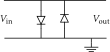
\includegraphics[scale=1.2]{report_img/diodes} 
		\caption{The double diode circuit is used to remove some of the amplitude of the signal before it is input to the mixer chip. This should allow a cleaner signal to be produced as the signal will be below the upper voltage limit of the chip.}
		\label{fig:diodes}
\end{figure} 

Another method to reduce the amplitude of the signal was attempted using a simple low pass filter. This time with a threshold frequency that is much higher than the wave which means that some of the frequencies that make up the square wave are removed. This will have the effect of reducing the overall amplitude of the wave, but at the expense of turning the square wave into a triangular wave. When implemented, this circuit had the desired effect of reducing the amplitude, but to such a degree that the signal is completely inaudible now. The amount of control over the properties of this circuit is limited and so this attempt is abandoned. 

\subsection{Quantitative Characteristics}
The nature of the variation of the produced signal with respect to the position of the user's hand is the product of several laws that govern separate components of the circuit. For example, the capacitance of the capacitor itself is inversely proportional to $d$ and the frequency of the oscillator chip is inversely proportional to $C$. This meant that the expect relation between the distance and the capacitance was
\begin{align}
	f &\propto \frac{1}{C} \propto \frac{1}{\frac{1}{d}} = d \nonumber \\
	\therefore f &\propto d 
\end{align}
This however was not seen when the frequency is measured with respect to the distance between the plates. When this was measured, shown in figure~\ref{fig:distance frequency}, the relation was found to be $f \propto \frac{1}{d}$.

\begin{figure}[ht]
	\centering
	\begin{minipage}[c]{0.3\textwidth}
		\begin{tabular}{r@{.}l|r@{.}l||r@{.}l|r@{.}l}
			\multicolumn{2}{c|}{\rotatebox{90}{Distance (cm)}} & \multicolumn{2}{c||}{\rotatebox{90}{Frequency (Hz)}} & \multicolumn{2}{c|}{\rotatebox{90}{Distance (cm)}} & \multicolumn{2}{c}{\rotatebox{90}{Frequency (Hz)}} \\ \hline \hline
			36&8	& 1&4 & 8&8	& 4&1 \\
			34&0	& 1&5 & 7&4	& 5&0 \\
			32&0	& 1&7 & 5&2	& 6&0 \\
			26&8	& 2&0 & 4&6	& 7&0 \\
			23&3	& 2&2 & 3&4	& 8&0 \\
			18&9	& 2&5 & 2&7	& 9&0 \\
			14&8	& 3&0 & 2&2	& 11&0 \\
			12&9	& 3&3 & 1&5	& 13&0 \\
			10&6	& 3&9 \\
		\end{tabular}
	\end{minipage}
	\begin{minipage}[c]{0.65\textwidth}
		\centering
		\centering
				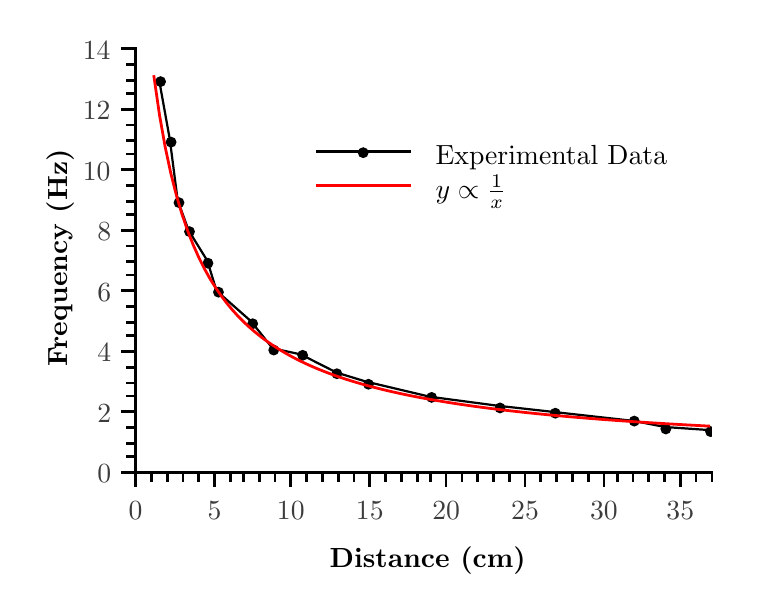
\begin{tikzpicture}{0pt}{0pt}{269pt}{209pt}
	\clip(0pt,209pt) -- (255.798pt,209pt) -- (255.798pt,10.2575pt) -- (0pt,10.2575pt) -- (0pt,209pt);
\begin{scope}
	\clip(38.9878pt,201.393pt) -- (247.239pt,201.393pt) -- (247.239pt,48.2943pt) -- (38.9878pt,48.2943pt) -- (38.9878pt,201.393pt);
	\color[rgb]{0,0,0}
	\draw[line width=0.8pt, line join=miter, line cap=rect](246.114pt,63.6042pt) -- (230.354pt,64.6977pt) -- (219.097pt,66.8848pt) -- (189.83pt,70.1655pt) -- (170.13pt,72.3526pt) -- (145.365pt,75.6333pt) -- (122.288pt,81.1011pt) -- (111.594pt,84.3818pt) -- (98.6491pt,90.9432pt) -- (88.5179pt,93.1303pt) -- (80.6381pt,102.972pt) -- (68.2556pt,113.908pt) -- (64.8785pt,124.843pt) -- (58.1244pt,135.779pt) -- (54.1845pt,146.715pt) -- (51.3703pt,168.586pt) -- (47.4304pt,190.457pt);
	\color[rgb]{0,0,0}
	\fill(246.764pt,63.0336pt) ellipse (1.42638pt and 1.42638pt);
	\draw[line width=1pt, line join=miter, line cap=rect](246.764pt,63.0336pt) ellipse (1.42638pt and 1.42638pt);
	\fill(230.598pt,63.9845pt) ellipse (1.42638pt and 1.42638pt);
	\draw[line width=1pt, line join=miter, line cap=rect](230.598pt,63.9845pt) ellipse (1.42638pt and 1.42638pt);
	\fill(219.187pt,66.8373pt) ellipse (1.42638pt and 1.42638pt);
	\draw[line width=1pt, line join=miter, line cap=rect](219.187pt,66.8373pt) ellipse (1.42638pt and 1.42638pt);
	\fill(190.66pt,69.6901pt) ellipse (1.42638pt and 1.42638pt);
	\draw[line width=1pt, line join=miter, line cap=rect](190.66pt,69.6901pt) ellipse (1.42638pt and 1.42638pt);
	\fill(170.69pt,71.5919pt) ellipse (1.42638pt and 1.42638pt);
	\draw[line width=1pt, line join=miter, line cap=rect](170.69pt,71.5919pt) ellipse (1.42638pt and 1.42638pt);
	\fill(145.966pt,75.3956pt) ellipse (1.42638pt and 1.42638pt);
	\draw[line width=1pt, line join=miter, line cap=rect](145.966pt,75.3956pt) ellipse (1.42638pt and 1.42638pt);
	\fill(123.144pt,80.1502pt) ellipse (1.42638pt and 1.42638pt);
	\draw[line width=1pt, line join=miter, line cap=rect](123.144pt,80.1502pt) ellipse (1.42638pt and 1.42638pt);
	\fill(111.733pt,83.9539pt) ellipse (1.42638pt and 1.42638pt);
	\draw[line width=1pt, line join=miter, line cap=rect](111.733pt,83.9539pt) ellipse (1.42638pt and 1.42638pt);
	\fill(99.3712pt,90.6103pt) ellipse (1.42638pt and 1.42638pt);
	\draw[line width=1pt, line join=miter, line cap=rect](99.3712pt,90.6103pt) ellipse (1.42638pt and 1.42638pt);
	\fill(88.9111pt,92.5122pt) ellipse (1.42638pt and 1.42638pt);
	\draw[line width=1pt, line join=miter, line cap=rect](88.9111pt,92.5122pt) ellipse (1.42638pt and 1.42638pt);
	\fill(81.3037pt,102.021pt) ellipse (1.42638pt and 1.42638pt);
	\draw[line width=1pt, line join=miter, line cap=rect](81.3037pt,102.021pt) ellipse (1.42638pt and 1.42638pt);
	\fill(68.9418pt,113.432pt) ellipse (1.42638pt and 1.42638pt);
	\draw[line width=1pt, line join=miter, line cap=rect](68.9418pt,113.432pt) ellipse (1.42638pt and 1.42638pt);
	\fill(65.1381pt,123.893pt) ellipse (1.42638pt and 1.42638pt);
	\draw[line width=1pt, line join=miter, line cap=rect](65.1381pt,123.893pt) ellipse (1.42638pt and 1.42638pt);
	\fill(58.4816pt,135.304pt) ellipse (1.42638pt and 1.42638pt);
	\draw[line width=1pt, line join=miter, line cap=rect](58.4816pt,135.304pt) ellipse (1.42638pt and 1.42638pt);
	\fill(54.678pt,145.764pt) ellipse (1.42638pt and 1.42638pt);
	\draw[line width=1pt, line join=miter, line cap=rect](54.678pt,145.764pt) ellipse (1.42638pt and 1.42638pt);
	\fill(51.8252pt,167.635pt) ellipse (1.42638pt and 1.42638pt);
	\draw[line width=1pt, line join=miter, line cap=rect](51.8252pt,167.635pt) ellipse (1.42638pt and 1.42638pt);
	\fill(48.0215pt,189.506pt) ellipse (1.42638pt and 1.42638pt);
	\draw[line width=1pt, line join=miter, line cap=rect](48.0215pt,189.506pt) ellipse (1.42638pt and 1.42638pt);
	\color[rgb]{1,0,0}
	\draw[line width=1pt, line join=bevel, line cap=rect](45.6293pt,191.317pt) -- (47.6544pt,177.335pt) -- (49.6795pt,165.934pt) -- (51.7046pt,156.458pt) -- (53.7297pt,148.459pt) -- (55.7548pt,141.616pt) -- (57.7799pt,135.695pt) -- (59.805pt,130.522pt) -- (61.8301pt,125.964pt) -- (63.8552pt,121.916pt) -- (65.8803pt,118.298pt) -- (67.9054pt,115.045pt) -- (69.9305pt,112.104pt) -- (71.9555pt,109.433pt) -- (73.9806pt,106.995pt) -- (76.0057pt,104.762pt) -- (78.0308pt,102.709pt) -- (80.0559pt,100.814pt) -- (82.081pt,99.0611pt) -- (84.1061pt,97.4339pt) -- (86.1312pt,95.9196pt) -- (88.1563pt,94.5067pt) -- (90.1814pt,93.1855pt) -- (92.2065pt,91.9472pt) -- (94.2316pt,90.7844pt) -- (96.2567pt,89.6903pt) -- (98.2818pt,88.659pt) -- (100.307pt,87.6853pt) -- (102.332pt,86.7644pt) -- (104.357pt,85.8922pt) -- (106.382pt,85.065pt) -- (108.407pt,84.2792pt) -- (110.432pt,83.5319pt) -- (112.457pt,82.8204pt) -- (114.483pt,82.1421pt) -- (116.508pt,81.4947pt) -- (118.533pt,80.8762pt) -- (120.558pt,80.2847pt) -- (122.583pt,79.7184pt) -- (124.608pt,79.1758pt) -- (126.633pt,78.6555pt) -- (128.658pt,78.156pt) -- (130.683pt,77.6762pt) -- (132.708pt,77.2148pt) -- (134.734pt,76.771pt) -- (136.759pt,76.3436pt) -- (138.784pt,75.9318pt) -- (140.809pt,75.5348pt) -- (142.834pt,75.1517pt) -- (144.859pt,74.7819pt) -- (146.884pt,74.4247pt) -- (148.909pt,74.0794pt) -- (150.934pt,73.7454pt) -- (152.959pt,73.4223pt) -- (154.984pt,73.1094pt) -- (157.01pt,72.8063pt) -- (159.035pt,72.5126pt) -- (161.06pt,72.2278pt) -- (163.085pt,71.9515pt) -- (165.11pt,71.6834pt) -- (167.135pt,71.4231pt) -- (169.16pt,71.1702pt) -- (171.185pt,70.9244pt) -- (173.21pt,70.6855pt) -- (175.235pt,70.4532pt) -- (177.261pt,70.2271pt) -- (179.286pt,70.0071pt) -- (181.311pt,69.7929pt) -- (183.336pt,69.5843pt) -- (185.361pt,69.381pt) -- (187.386pt,69.1829pt) -- (189.411pt,68.9898pt) -- (191.436pt,68.8014pt) -- (193.461pt,68.6176pt) -- (195.486pt,68.4383pt) -- (197.511pt,68.2632pt) -- (199.537pt,68.0923pt) -- (201.562pt,67.9254pt) -- (203.587pt,67.7623pt) -- (205.612pt,67.6029pt) -- (207.637pt,67.4471pt) -- (209.662pt,67.2948pt) -- (211.687pt,67.1458pt) -- (213.712pt,67.0001pt) -- (215.737pt,66.8575pt) -- (217.762pt,66.7179pt) -- (219.788pt,66.5813pt) -- (221.813pt,66.4475pt) -- (223.838pt,66.3166pt) -- (225.863pt,66.1882pt) -- (227.888pt,66.0625pt) -- (229.913pt,65.9393pt) -- (231.938pt,65.8186pt) -- (233.963pt,65.7002pt) -- (235.988pt,65.5841pt) -- (238.013pt,65.4702pt) -- (240.039pt,65.3586pt) -- (242.064pt,65.249pt) -- (244.089pt,65.1415pt) -- (246.114pt,65.0359pt);
\end{scope}
\begin{scope}
	\color[rgb]{0,0,0}
	\pgftext[center, base, at={\pgfpoint{14.2638pt}{125.794pt}},rotate=90]{\textbf{Frequency (Hz)}}
	\color[rgb]{0.235294,0.235294,0.235294}
	\pgftext[center, base, at={\pgfpoint{27.6881pt}{44.4907pt}}]{0}
	\pgftext[center, base, at={\pgfpoint{27.6881pt}{66.3618pt}}]{2}
	\pgftext[center, base, at={\pgfpoint{27.6881pt}{88.233pt}}]{4}
	\pgftext[center, base, at={\pgfpoint{27.6881pt}{110.104pt}}]{6}
	\pgftext[center, base, at={\pgfpoint{27.6881pt}{131.975pt}}]{8}
	\pgftext[center, base, at={\pgfpoint{24.9468pt}{153.847pt}}]{10}
	\pgftext[center, base, at={\pgfpoint{24.9468pt}{175.718pt}}]{12}
	\pgftext[center, base, at={\pgfpoint{24.9468pt}{197.589pt}}]{14}
	\color[rgb]{0,0,0}
	\draw[line width=1pt, line join=bevel, line cap=rect](38.9878pt,53.9999pt) -- (36.135pt,53.9999pt);
	\draw[line width=1pt, line join=bevel, line cap=rect](38.9878pt,64.46pt) -- (36.135pt,64.46pt);
	\draw[line width=1pt, line join=bevel, line cap=rect](38.9878pt,75.8711pt) -- (36.135pt,75.8711pt);
	\draw[line width=1pt, line join=bevel, line cap=rect](38.9878pt,86.3312pt) -- (36.135pt,86.3312pt);
	\draw[line width=1pt, line join=bevel, line cap=rect](38.9878pt,97.7422pt) -- (36.135pt,97.7422pt);
	\draw[line width=1pt, line join=bevel, line cap=rect](38.9878pt,108.202pt) -- (36.135pt,108.202pt);
	\draw[line width=1pt, line join=bevel, line cap=rect](38.9878pt,119.613pt) -- (36.135pt,119.613pt);
	\draw[line width=1pt, line join=bevel, line cap=rect](38.9878pt,130.074pt) -- (36.135pt,130.074pt);
	\draw[line width=1pt, line join=bevel, line cap=rect](38.9878pt,141.485pt) -- (36.135pt,141.485pt);
	\draw[line width=1pt, line join=bevel, line cap=rect](38.9878pt,151.945pt) -- (36.135pt,151.945pt);
	\draw[line width=1pt, line join=bevel, line cap=rect](38.9878pt,163.356pt) -- (36.135pt,163.356pt);
	\draw[line width=1pt, line join=bevel, line cap=rect](38.9878pt,173.816pt) -- (36.135pt,173.816pt);
	\draw[line width=1pt, line join=bevel, line cap=rect](38.9878pt,185.227pt) -- (36.135pt,185.227pt);
	\draw[line width=1pt, line join=bevel, line cap=rect](38.9878pt,195.687pt) -- (36.135pt,195.687pt);
	\draw[line width=1pt, line join=bevel, line cap=rect](38.9878pt,58.7545pt) -- (36.135pt,58.7545pt);
	\draw[line width=1pt, line join=bevel, line cap=rect](38.9878pt,80.6257pt) -- (36.135pt,80.6257pt);
	\draw[line width=1pt, line join=bevel, line cap=rect](38.9878pt,102.497pt) -- (36.135pt,102.497pt);
	\draw[line width=1pt, line join=bevel, line cap=rect](38.9878pt,124.368pt) -- (36.135pt,124.368pt);
	\draw[line width=1pt, line join=bevel, line cap=rect](38.9878pt,146.239pt) -- (36.135pt,146.239pt);
	\draw[line width=1pt, line join=bevel, line cap=rect](38.9878pt,168.11pt) -- (36.135pt,168.11pt);
	\draw[line width=1pt, line join=bevel, line cap=rect](38.9878pt,189.982pt) -- (36.135pt,189.982pt);
	\draw[line width=1pt, line join=bevel, line cap=rect](38.9878pt,48.2943pt) -- (34.2332pt,48.2943pt);
	\draw[line width=1pt, line join=bevel, line cap=rect](38.9878pt,70.1655pt) -- (34.2332pt,70.1655pt);
	\draw[line width=1pt, line join=bevel, line cap=rect](38.9878pt,92.0367pt) -- (34.2332pt,92.0367pt);
	\draw[line width=1pt, line join=bevel, line cap=rect](38.9878pt,113.908pt) -- (34.2332pt,113.908pt);
	\draw[line width=1pt, line join=bevel, line cap=rect](38.9878pt,135.779pt) -- (34.2332pt,135.779pt);
	\draw[line width=1pt, line join=bevel, line cap=rect](38.9878pt,157.65pt) -- (34.2332pt,157.65pt);
	\draw[line width=1pt, line join=bevel, line cap=rect](38.9878pt,179.521pt) -- (34.2332pt,179.521pt);
	\draw[line width=1pt, line join=bevel, line cap=rect](38.9878pt,201.393pt) -- (34.2332pt,201.393pt);
	\draw[line width=1pt, line join=bevel, line cap=rect](38.9878pt,201.393pt) -- (38.9878pt,48.2943pt);
	\pgftext[center, base, at={\pgfpoint{144.533pt}{14.0612pt}}]{\textbf{Distance (cm)}}
	\color[rgb]{0.235294,0.235294,0.235294}
	\pgftext[center, base, at={\pgfpoint{38.9803pt}{31.1778pt}}]{0}
	\pgftext[center, base, at={\pgfpoint{67.508pt}{31.1778pt}}]{5}
	\pgftext[center, base, at={\pgfpoint{95.0921pt}{31.1778pt}}]{10}
	\pgftext[center, base, at={\pgfpoint{123.62pt}{31.1778pt}}]{15}
	\pgftext[center, base, at={\pgfpoint{151.196pt}{31.1778pt}}]{20}
	\pgftext[center, base, at={\pgfpoint{179.724pt}{31.1778pt}}]{25}
	\pgftext[center, base, at={\pgfpoint{208.252pt}{31.1778pt}}]{30}
	\pgftext[center, base, at={\pgfpoint{235.828pt}{31.1778pt}}]{35}
	\color[rgb]{0,0,0}
	\draw[line width=1pt, line join=bevel, line cap=rect](44.6933pt,48.2943pt) -- (44.6933pt,45.4416pt);
	\draw[line width=1pt, line join=bevel, line cap=rect](50.3988pt,48.2943pt) -- (50.3988pt,45.4416pt);
	\draw[line width=1pt, line join=bevel, line cap=rect](56.1043pt,48.2943pt) -- (56.1043pt,45.4416pt);
	\draw[line width=1pt, line join=bevel, line cap=rect](61.8099pt,48.2943pt) -- (61.8099pt,45.4416pt);
	\draw[line width=1pt, line join=bevel, line cap=rect](73.2209pt,48.2943pt) -- (73.2209pt,45.4416pt);
	\draw[line width=1pt, line join=bevel, line cap=rect](77.9755pt,48.2943pt) -- (77.9755pt,45.4416pt);
	\draw[line width=1pt, line join=bevel, line cap=rect](83.6811pt,48.2943pt) -- (83.6811pt,45.4416pt);
	\draw[line width=1pt, line join=bevel, line cap=rect](89.3866pt,48.2943pt) -- (89.3866pt,45.4416pt);
	\draw[line width=1pt, line join=bevel, line cap=rect](100.798pt,48.2943pt) -- (100.798pt,45.4416pt);
	\draw[line width=1pt, line join=bevel, line cap=rect](106.503pt,48.2943pt) -- (106.503pt,45.4416pt);
	\draw[line width=1pt, line join=bevel, line cap=rect](112.209pt,48.2943pt) -- (112.209pt,45.4416pt);
	\draw[line width=1pt, line join=bevel, line cap=rect](117.914pt,48.2943pt) -- (117.914pt,45.4416pt);
	\draw[line width=1pt, line join=bevel, line cap=rect](129.325pt,48.2943pt) -- (129.325pt,45.4416pt);
	\draw[line width=1pt, line join=bevel, line cap=rect](135.031pt,48.2943pt) -- (135.031pt,45.4416pt);
	\draw[line width=1pt, line join=bevel, line cap=rect](140.736pt,48.2943pt) -- (140.736pt,45.4416pt);
	\draw[line width=1pt, line join=bevel, line cap=rect](145.491pt,48.2943pt) -- (145.491pt,45.4416pt);
	\draw[line width=1pt, line join=bevel, line cap=rect](156.902pt,48.2943pt) -- (156.902pt,45.4416pt);
	\draw[line width=1pt, line join=bevel, line cap=rect](162.607pt,48.2943pt) -- (162.607pt,45.4416pt);
	\draw[line width=1pt, line join=bevel, line cap=rect](168.313pt,48.2943pt) -- (168.313pt,45.4416pt);
	\draw[line width=1pt, line join=bevel, line cap=rect](174.019pt,48.2943pt) -- (174.019pt,45.4416pt);
	\draw[line width=1pt, line join=bevel, line cap=rect](185.43pt,48.2943pt) -- (185.43pt,45.4416pt);
	\draw[line width=1pt, line join=bevel, line cap=rect](191.135pt,48.2943pt) -- (191.135pt,45.4416pt);
	\draw[line width=1pt, line join=bevel, line cap=rect](196.841pt,48.2943pt) -- (196.841pt,45.4416pt);
	\draw[line width=1pt, line join=bevel, line cap=rect](202.546pt,48.2943pt) -- (202.546pt,45.4416pt);
	\draw[line width=1pt, line join=bevel, line cap=rect](213.006pt,48.2943pt) -- (213.006pt,45.4416pt);
	\draw[line width=1pt, line join=bevel, line cap=rect](218.712pt,48.2943pt) -- (218.712pt,45.4416pt);
	\draw[line width=1pt, line join=bevel, line cap=rect](224.417pt,48.2943pt) -- (224.417pt,45.4416pt);
	\draw[line width=1pt, line join=bevel, line cap=rect](230.123pt,48.2943pt) -- (230.123pt,45.4416pt);
	\draw[line width=1pt, line join=bevel, line cap=rect](241.534pt,48.2943pt) -- (241.534pt,45.4416pt);
	\draw[line width=1pt, line join=bevel, line cap=rect](247.239pt,48.2943pt) -- (247.239pt,45.4416pt);
	\draw[line width=1pt, line join=bevel, line cap=rect](38.9878pt,48.2943pt) -- (38.9878pt,43.5397pt);
	\draw[line width=1pt, line join=bevel, line cap=rect](67.5154pt,48.2943pt) -- (67.5154pt,43.5397pt);
	\draw[line width=1pt, line join=bevel, line cap=rect](95.0921pt,48.2943pt) -- (95.0921pt,43.5397pt);
	\draw[line width=1pt, line join=bevel, line cap=rect](123.62pt,48.2943pt) -- (123.62pt,43.5397pt);
	\draw[line width=1pt, line join=bevel, line cap=rect](151.196pt,48.2943pt) -- (151.196pt,43.5397pt);
	\draw[line width=1pt, line join=bevel, line cap=rect](179.724pt,48.2943pt) -- (179.724pt,43.5397pt);
	\draw[line width=1pt, line join=bevel, line cap=rect](208.252pt,48.2943pt) -- (208.252pt,43.5397pt);
	\draw[line width=1pt, line join=bevel, line cap=rect](235.828pt,48.2943pt) -- (235.828pt,43.5397pt);
	\draw[line width=1pt, line join=bevel, line cap=rect](38.9878pt,48.2943pt) -- (247.239pt,48.2943pt);
	\draw[line width=1pt, line join=miter, line cap=rect](104.601pt,164.307pt) -- (137.884pt,164.307pt);
	\fill(121.242pt,163.831pt) ellipse (1.42638pt and 1.42638pt);
	\draw[line width=1pt, line join=miter, line cap=rect](121.242pt,163.831pt) ellipse (1.42638pt and 1.42638pt);
	\pgftext[left, base, at={\pgfpoint{147.393pt}{159.552pt}}]{Experimental Data}
	\color[rgb]{1,0,0}
	\draw[line width=1pt, line join=bevel, line cap=rect](104.601pt,151.945pt) -- (137.884pt,151.945pt);
	\color[rgb]{0,0,0}
	\pgftext[left, base, at={\pgfpoint{147.393pt}{147.19pt}}]{$y \propto \frac{1}{x}$}
\end{scope}
\end{tikzpicture}
 
			\vspace{-10pt}
	\end{minipage}
	\caption{The distance from the plate capacitor against the frequency that this position produces is recorded.}
	\label{fig:distance frequency}
\end{figure}

Also, the action of the mixer chip was verified by measuring the output frequency produced when using a single VCO at a fixed frequency of 1.5\,MHz and the variable TG315 signal generator. This is shown in figure~\ref{fig:frequency generator}. The linear direct relationship can be clearly seen here. This graph is of the form $y=|x-c|$ where $c$ is a constant, since the two regions have the same slope. This confirms that the action of the mixer is as expected.  

\begin{figure}
	\begin{center}
		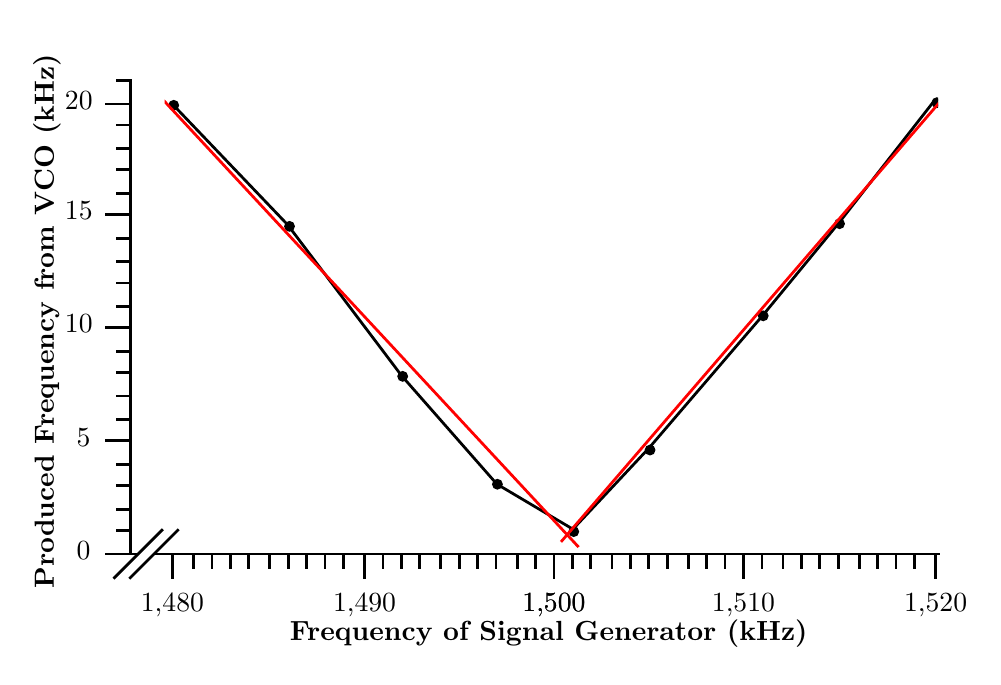
\begin{tikzpicture}{0pt}{0pt}{359pt}{239pt}
	\clip(0pt,239pt) -- (341.381pt,239pt) -- (341.381pt,11.7299pt) -- (0pt,11.7299pt) -- (0pt,239pt);
\begin{scope}
	\clip(49.4479pt,219.982pt) -- (329.019pt,219.982pt) -- (329.019pt,48.8158pt) -- (49.4479pt,48.8158pt) -- (49.4479pt,219.982pt);
	\color[rgb]{0,0,0}
	\draw[line width=1pt, line join=miter, line cap=rect](52.6521pt,211.016pt) -- (93.9009pt,167.817pt) -- (135.15pt,113.207pt) -- (169.524pt,74.0831pt) -- (197.023pt,57.7816pt) -- (224.522pt,87.1243pt) -- (265.771pt,135.214pt) -- (293.27pt,168.632pt) -- (327.644pt,212.646pt);
	\color[rgb]{0,0,0}
	\fill(52.7761pt,210.948pt) ellipse (1.42638pt and 1.42638pt);
	\draw[line width=1pt, line join=miter, line cap=rect](52.7761pt,210.948pt) ellipse (1.42638pt and 1.42638pt);
	\fill(94.6166pt,167.205pt) ellipse (1.42638pt and 1.42638pt);
	\draw[line width=1pt, line join=miter, line cap=rect](94.6166pt,167.205pt) ellipse (1.42638pt and 1.42638pt);
	\fill(135.506pt,113.003pt) ellipse (1.42638pt and 1.42638pt);
	\draw[line width=1pt, line join=miter, line cap=rect](135.506pt,113.003pt) ellipse (1.42638pt and 1.42638pt);
	\fill(169.739pt,74.0152pt) ellipse (1.42638pt and 1.42638pt);
	\draw[line width=1pt, line join=miter, line cap=rect](169.739pt,74.0152pt) ellipse (1.42638pt and 1.42638pt);
	\fill(197.316pt,56.8986pt) ellipse (1.42638pt and 1.42638pt);
	\draw[line width=1pt, line join=miter, line cap=rect](197.316pt,56.8986pt) ellipse (1.42638pt and 1.42638pt);
	\fill(224.893pt,86.3772pt) ellipse (1.42638pt and 1.42638pt);
	\draw[line width=1pt, line join=miter, line cap=rect](224.893pt,86.3772pt) ellipse (1.42638pt and 1.42638pt);
	\fill(265.782pt,134.874pt) ellipse (1.42638pt and 1.42638pt);
	\draw[line width=1pt, line join=miter, line cap=rect](265.782pt,134.874pt) ellipse (1.42638pt and 1.42638pt);
	\fill(293.359pt,168.156pt) ellipse (1.42638pt and 1.42638pt);
	\draw[line width=1pt, line join=miter, line cap=rect](293.359pt,168.156pt) ellipse (1.42638pt and 1.42638pt);
	\fill(328.543pt,211.899pt) ellipse (1.42638pt and 1.42638pt);
	\draw[line width=1pt, line join=miter, line cap=rect](328.543pt,211.899pt) ellipse (1.42638pt and 1.42638pt);
	\color[rgb]{1,0,0}
	\draw[line width=1pt, line join=miter, line cap=rect](334.724pt,218.08pt) -- (193.037pt,53.5704pt);
	\draw[line width=1pt, line join=miter, line cap=rect](49.4479pt,212.374pt) -- (198.742pt,51.6686pt);
\end{scope}
\begin{scope}
	\color[rgb]{0,0,0}
	\pgftext[center, base, at={\pgfpoint{188.275pt}{227.589pt}}]{\textbf{ }}
	\color[rgb]{0,0,0}
	\pgftext[center, base, at={\pgfpoint{9.50921pt}{132.972pt}},rotate=90]{\textbf{Produced Frequency from VCO (kHz)}}
	\pgftext[center, base, at={\pgfpoint{20.1774pt}{46.9139pt}}]{0}
	\pgftext[center, base, at={\pgfpoint{20.1774pt}{87.8036pt}}]{5}
	\pgftext[center, base, at={\pgfpoint{18.4835pt}{128.693pt}}]{10}
	\pgftext[center, base, at={\pgfpoint{18.4835pt}{169.583pt}}]{15}
	\pgftext[center, base, at={\pgfpoint{18.4835pt}{209.521pt}}]{20}
	\draw[line width=1pt, line join=bevel, line cap=rect](37.0859pt,57.3741pt) -- (32.3313pt,57.3741pt);
	\draw[line width=1pt, line join=bevel, line cap=rect](37.0859pt,64.9814pt) -- (32.3313pt,64.9814pt);
	\draw[line width=1pt, line join=bevel, line cap=rect](37.0859pt,73.5397pt) -- (32.3313pt,73.5397pt);
	\draw[line width=1pt, line join=bevel, line cap=rect](37.0859pt,81.1471pt) -- (32.3313pt,81.1471pt);
	\draw[line width=1pt, line join=bevel, line cap=rect](37.0859pt,97.3128pt) -- (32.3313pt,97.3128pt);
	\draw[line width=1pt, line join=bevel, line cap=rect](37.0859pt,105.871pt) -- (32.3313pt,105.871pt);
	\draw[line width=1pt, line join=bevel, line cap=rect](37.0859pt,114.429pt) -- (32.3313pt,114.429pt);
	\draw[line width=1pt, line join=bevel, line cap=rect](37.0859pt,122.037pt) -- (32.3313pt,122.037pt);
	\draw[line width=1pt, line join=bevel, line cap=rect](37.0859pt,138.202pt) -- (32.3313pt,138.202pt);
	\draw[line width=1pt, line join=bevel, line cap=rect](37.0859pt,146.761pt) -- (32.3313pt,146.761pt);
	\draw[line width=1pt, line join=bevel, line cap=rect](37.0859pt,154.368pt) -- (32.3313pt,154.368pt);
	\draw[line width=1pt, line join=bevel, line cap=rect](37.0859pt,162.926pt) -- (32.3313pt,162.926pt);
	\draw[line width=1pt, line join=bevel, line cap=rect](37.0859pt,179.092pt) -- (32.3313pt,179.092pt);
	\draw[line width=1pt, line join=bevel, line cap=rect](37.0859pt,187.65pt) -- (32.3313pt,187.65pt);
	\draw[line width=1pt, line join=bevel, line cap=rect](37.0859pt,195.258pt) -- (32.3313pt,195.258pt);
	\draw[line width=1pt, line join=bevel, line cap=rect](37.0859pt,203.816pt) -- (32.3313pt,203.816pt);
	\draw[line width=1pt, line join=bevel, line cap=rect](37.0859pt,219.982pt) -- (32.3313pt,219.982pt);
	\draw[line width=1pt, line join=bevel, line cap=rect](37.0859pt,48.8158pt) -- (28.5276pt,48.8158pt);
	\draw[line width=1pt, line join=bevel, line cap=rect](37.0859pt,89.7054pt) -- (28.5276pt,89.7054pt);
	\draw[line width=1pt, line join=bevel, line cap=rect](37.0859pt,130.595pt) -- (28.5276pt,130.595pt);
	\draw[line width=1pt, line join=bevel, line cap=rect](37.0859pt,171.485pt) -- (28.5276pt,171.485pt);
	\draw[line width=1pt, line join=bevel, line cap=rect](37.0859pt,211.423pt) -- (28.5276pt,211.423pt);
	\draw[line width=1pt, line join=bevel, line cap=rect](37.0859pt,219.982pt) -- (37.0859pt,48.8158pt);
	\pgftext[center, base, at={\pgfpoint{188.275pt}{17.4354pt}}]{\textbf{Frequency of Signal Generator (kHz)}}
	\draw[line width=1pt, line join=bevel, line cap=rect](48.497pt,57.3741pt) -- (31.3804pt,40.2575pt);
	\draw[line width=1pt, line join=bevel, line cap=rect](54.2025pt,57.3741pt) -- (37.0859pt,40.2575pt);
	\pgftext[center, base, at={\pgfpoint{190.184pt}{27.8955pt}}]{1,500}
	\pgftext[center, base, at={\pgfpoint{52.3007pt}{27.8955pt}}]{1,480}
	\pgftext[center, base, at={\pgfpoint{121.718pt}{27.8955pt}}]{1,490}
	\pgftext[center, base, at={\pgfpoint{190.184pt}{27.8955pt}}]{1,500}
	\pgftext[center, base, at={\pgfpoint{258.651pt}{27.8955pt}}]{1,510}
	\pgftext[center, base, at={\pgfpoint{328.068pt}{27.8955pt}}]{1,520}
	\draw[line width=1pt, line join=bevel, line cap=rect](59.908pt,48.8158pt) -- (59.908pt,44.0612pt);
	\draw[line width=1pt, line join=bevel, line cap=rect](66.5645pt,48.8158pt) -- (66.5645pt,44.0612pt);
	\draw[line width=1pt, line join=bevel, line cap=rect](73.2209pt,48.8158pt) -- (73.2209pt,44.0612pt);
	\draw[line width=1pt, line join=bevel, line cap=rect](79.8774pt,48.8158pt) -- (79.8774pt,44.0612pt);
	\draw[line width=1pt, line join=bevel, line cap=rect](94.1412pt,48.8158pt) -- (94.1412pt,44.0612pt);
	\draw[line width=1pt, line join=bevel, line cap=rect](100.798pt,48.8158pt) -- (100.798pt,44.0612pt);
	\draw[line width=1pt, line join=bevel, line cap=rect](107.454pt,48.8158pt) -- (107.454pt,44.0612pt);
	\draw[line width=1pt, line join=bevel, line cap=rect](114.111pt,48.8158pt) -- (114.111pt,44.0612pt);
	\draw[line width=1pt, line join=bevel, line cap=rect](128.374pt,48.8158pt) -- (128.374pt,44.0612pt);
	\draw[line width=1pt, line join=bevel, line cap=rect](135.031pt,48.8158pt) -- (135.031pt,44.0612pt);
	\draw[line width=1pt, line join=bevel, line cap=rect](141.687pt,48.8158pt) -- (141.687pt,44.0612pt);
	\draw[line width=1pt, line join=bevel, line cap=rect](149.295pt,48.8158pt) -- (149.295pt,44.0612pt);
	\draw[line width=1pt, line join=bevel, line cap=rect](162.607pt,48.8158pt) -- (162.607pt,44.0612pt);
	\draw[line width=1pt, line join=bevel, line cap=rect](169.264pt,48.8158pt) -- (169.264pt,44.0612pt);
	\draw[line width=1pt, line join=bevel, line cap=rect](176.871pt,48.8158pt) -- (176.871pt,44.0612pt);
	\draw[line width=1pt, line join=bevel, line cap=rect](183.528pt,48.8158pt) -- (183.528pt,44.0612pt);
	\draw[line width=1pt, line join=bevel, line cap=rect](196.841pt,48.8158pt) -- (196.841pt,44.0612pt);
	\draw[line width=1pt, line join=bevel, line cap=rect](203.497pt,48.8158pt) -- (203.497pt,44.0612pt);
	\draw[line width=1pt, line join=bevel, line cap=rect](211.104pt,48.8158pt) -- (211.104pt,44.0612pt);
	\draw[line width=1pt, line join=bevel, line cap=rect](217.761pt,48.8158pt) -- (217.761pt,44.0612pt);
	\draw[line width=1pt, line join=bevel, line cap=rect](231.074pt,48.8158pt) -- (231.074pt,44.0612pt);
	\draw[line width=1pt, line join=bevel, line cap=rect](238.681pt,48.8158pt) -- (238.681pt,44.0612pt);
	\draw[line width=1pt, line join=bevel, line cap=rect](245.338pt,48.8158pt) -- (245.338pt,44.0612pt);
	\draw[line width=1pt, line join=bevel, line cap=rect](251.994pt,48.8158pt) -- (251.994pt,44.0612pt);
	\draw[line width=1pt, line join=bevel, line cap=rect](265.307pt,48.8158pt) -- (265.307pt,44.0612pt);
	\draw[line width=1pt, line join=bevel, line cap=rect](272.914pt,48.8158pt) -- (272.914pt,44.0612pt);
	\draw[line width=1pt, line join=bevel, line cap=rect](279.571pt,48.8158pt) -- (279.571pt,44.0612pt);
	\draw[line width=1pt, line join=bevel, line cap=rect](286.227pt,48.8158pt) -- (286.227pt,44.0612pt);
	\draw[line width=1pt, line join=bevel, line cap=rect](300.491pt,48.8158pt) -- (300.491pt,44.0612pt);
	\draw[line width=1pt, line join=bevel, line cap=rect](307.147pt,48.8158pt) -- (307.147pt,44.0612pt);
	\draw[line width=1pt, line join=bevel, line cap=rect](313.804pt,48.8158pt) -- (313.804pt,44.0612pt);
	\draw[line width=1pt, line join=bevel, line cap=rect](320.46pt,48.8158pt) -- (320.46pt,44.0612pt);
	\draw[line width=1pt, line join=bevel, line cap=rect](87.4847pt,48.8158pt) -- (87.4847pt,44.0612pt);
	\draw[line width=1pt, line join=bevel, line cap=rect](155.951pt,48.8158pt) -- (155.951pt,44.0612pt);
	\draw[line width=1pt, line join=bevel, line cap=rect](224.417pt,48.8158pt) -- (224.417pt,44.0612pt);
	\draw[line width=1pt, line join=bevel, line cap=rect](292.884pt,48.8158pt) -- (292.884pt,44.0612pt);
	\draw[line width=1pt, line join=bevel, line cap=rect](190.184pt,48.8158pt) -- (190.184pt,40.2575pt);
	\draw[line width=1pt, line join=bevel, line cap=rect](52.3007pt,48.8158pt) -- (52.3007pt,40.2575pt);
	\draw[line width=1pt, line join=bevel, line cap=rect](121.718pt,48.8158pt) -- (121.718pt,40.2575pt);
	\draw[line width=1pt, line join=bevel, line cap=rect](190.184pt,48.8158pt) -- (190.184pt,40.2575pt);
	\draw[line width=1pt, line join=bevel, line cap=rect](258.651pt,48.8158pt) -- (258.651pt,40.2575pt);
	\draw[line width=1pt, line join=bevel, line cap=rect](328.068pt,48.8158pt) -- (328.068pt,40.2575pt);
	\draw[line width=1pt, line join=bevel, line cap=rect](37.0859pt,48.8158pt) -- (38.9878pt,48.8158pt);
	\draw[line width=1pt, line join=bevel, line cap=rect](46.5951pt,48.8158pt) -- (329.019pt,48.8158pt);
\end{scope}
\end{tikzpicture}

		\caption{As the generator input frequency to the mixer is increased, the difference between the generator and the reference VCO decreases, and so does the output frequency produced, until the generator is greater than the reference and so the difference, and so the output frequency, increases.}
		\label{fig:frequency generator}
	\end{center}
\end{figure}

Finally the relationship between the frequency of the input to the low pass circuit and the peak to peak voltage of the output of low pass circuit was measured. This allowed the characteristics of the signal with respect to the voltage to be observed. As can be seen in figure~\ref{fig:bode}, this is essentially a Bode plot with a cut off frequency of around 23.5\,kHz, just above human hearing range. This confirmed what was expected. As the frequency increases, the voltage is almost constant, up until the cut off frequency where the voltage is attenuated swiftly. This is due to the effect of the low pass filter removing the high frequency signals as desired.

\begin{figure}
	\begin{center}
		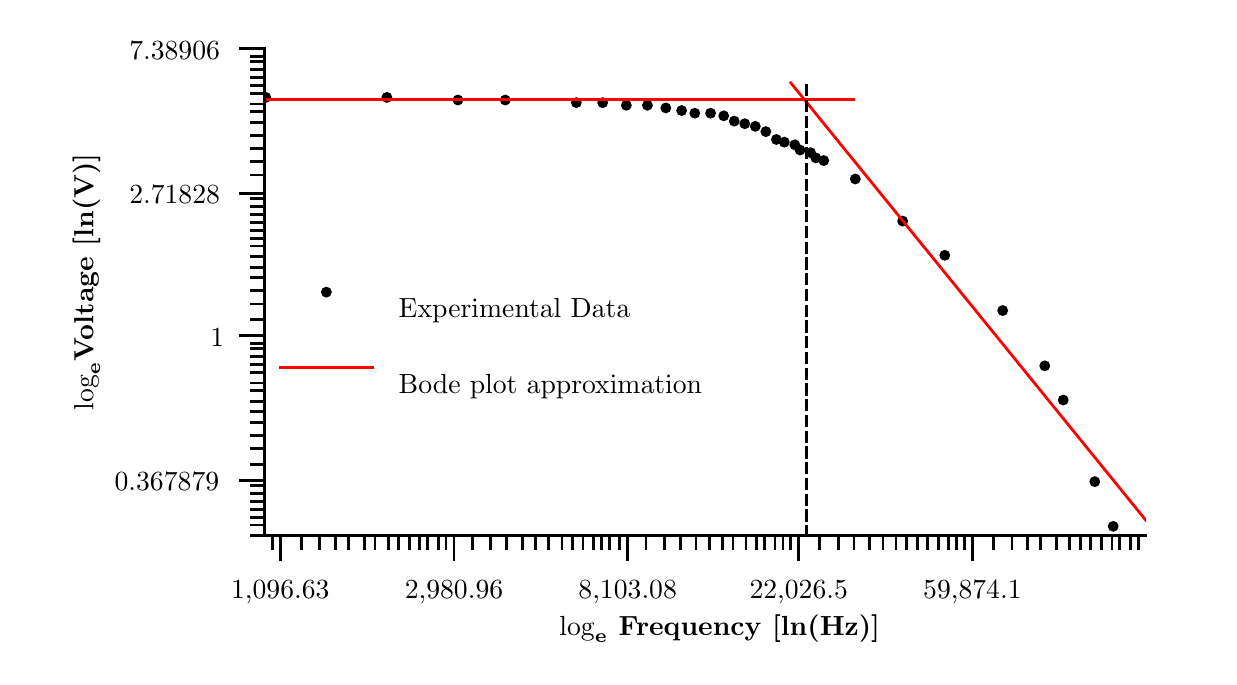
\begin{tikzpicture}{0pt}{0pt}{449pt}{239pt}
	\clip(0pt,239pt) -- (426.964pt,239pt) -- (426.964pt,11.7299pt) -- (0pt,11.7299pt) -- (0pt,239pt);
\begin{scope}
	\clip(85.5829pt,231.393pt) -- (404.141pt,231.393pt) -- (404.141pt,55.4722pt) -- (85.5829pt,55.4722pt) -- (85.5829pt,231.393pt);
	\color[rgb]{0,0,0}
	\fill(86.0584pt,213.801pt) ellipse (1.42638pt and 1.42638pt);
	\draw[line width=1pt, line join=miter, line cap=rect](86.0584pt,213.801pt) ellipse (1.42638pt and 1.42638pt);
	\color[rgb]{0,0,0}
	\fill(129.801pt,213.801pt) ellipse (1.42638pt and 1.42638pt);
	\draw[line width=1pt, line join=miter, line cap=rect](129.801pt,213.801pt) ellipse (1.42638pt and 1.42638pt);
	\fill(155.476pt,212.85pt) ellipse (1.42638pt and 1.42638pt);
	\draw[line width=1pt, line join=miter, line cap=rect](155.476pt,212.85pt) ellipse (1.42638pt and 1.42638pt);
	\fill(172.592pt,212.85pt) ellipse (1.42638pt and 1.42638pt);
	\draw[line width=1pt, line join=miter, line cap=rect](172.592pt,212.85pt) ellipse (1.42638pt and 1.42638pt);
	\fill(198.267pt,211.899pt) ellipse (1.42638pt and 1.42638pt);
	\draw[line width=1pt, line join=miter, line cap=rect](198.267pt,211.899pt) ellipse (1.42638pt and 1.42638pt);
	\fill(207.776pt,211.899pt) ellipse (1.42638pt and 1.42638pt);
	\draw[line width=1pt, line join=miter, line cap=rect](207.776pt,211.899pt) ellipse (1.42638pt and 1.42638pt);
	\fill(216.335pt,210.948pt) ellipse (1.42638pt and 1.42638pt);
	\draw[line width=1pt, line join=miter, line cap=rect](216.335pt,210.948pt) ellipse (1.42638pt and 1.42638pt);
	\fill(223.942pt,210.948pt) ellipse (1.42638pt and 1.42638pt);
	\draw[line width=1pt, line join=miter, line cap=rect](223.942pt,210.948pt) ellipse (1.42638pt and 1.42638pt);
	\fill(230.598pt,209.997pt) ellipse (1.42638pt and 1.42638pt);
	\draw[line width=1pt, line join=miter, line cap=rect](230.598pt,209.997pt) ellipse (1.42638pt and 1.42638pt);
	\fill(236.304pt,209.046pt) ellipse (1.42638pt and 1.42638pt);
	\draw[line width=1pt, line join=miter, line cap=rect](236.304pt,209.046pt) ellipse (1.42638pt and 1.42638pt);
	\fill(241.058pt,208.095pt) ellipse (1.42638pt and 1.42638pt);
	\draw[line width=1pt, line join=miter, line cap=rect](241.058pt,208.095pt) ellipse (1.42638pt and 1.42638pt);
	\fill(246.764pt,208.095pt) ellipse (1.42638pt and 1.42638pt);
	\draw[line width=1pt, line join=miter, line cap=rect](246.764pt,208.095pt) ellipse (1.42638pt and 1.42638pt);
	\fill(251.519pt,207.144pt) ellipse (1.42638pt and 1.42638pt);
	\draw[line width=1pt, line join=miter, line cap=rect](251.519pt,207.144pt) ellipse (1.42638pt and 1.42638pt);
	\fill(255.322pt,205.242pt) ellipse (1.42638pt and 1.42638pt);
	\draw[line width=1pt, line join=miter, line cap=rect](255.322pt,205.242pt) ellipse (1.42638pt and 1.42638pt);
	\fill(259.126pt,204.291pt) ellipse (1.42638pt and 1.42638pt);
	\draw[line width=1pt, line join=miter, line cap=rect](259.126pt,204.291pt) ellipse (1.42638pt and 1.42638pt);
	\fill(262.93pt,203.34pt) ellipse (1.42638pt and 1.42638pt);
	\draw[line width=1pt, line join=miter, line cap=rect](262.93pt,203.34pt) ellipse (1.42638pt and 1.42638pt);
	\fill(266.733pt,201.439pt) ellipse (1.42638pt and 1.42638pt);
	\draw[line width=1pt, line join=miter, line cap=rect](266.733pt,201.439pt) ellipse (1.42638pt and 1.42638pt);
	\fill(270.537pt,198.586pt) ellipse (1.42638pt and 1.42638pt);
	\draw[line width=1pt, line join=miter, line cap=rect](270.537pt,198.586pt) ellipse (1.42638pt and 1.42638pt);
	\fill(273.39pt,197.635pt) ellipse (1.42638pt and 1.42638pt);
	\draw[line width=1pt, line join=miter, line cap=rect](273.39pt,197.635pt) ellipse (1.42638pt and 1.42638pt);
	\fill(277.193pt,196.684pt) ellipse (1.42638pt and 1.42638pt);
	\draw[line width=1pt, line join=miter, line cap=rect](277.193pt,196.684pt) ellipse (1.42638pt and 1.42638pt);
	\fill(279.095pt,194.782pt) ellipse (1.42638pt and 1.42638pt);
	\draw[line width=1pt, line join=miter, line cap=rect](279.095pt,194.782pt) ellipse (1.42638pt and 1.42638pt);
	\fill(282.899pt,193.831pt) ellipse (1.42638pt and 1.42638pt);
	\draw[line width=1pt, line join=miter, line cap=rect](282.899pt,193.831pt) ellipse (1.42638pt and 1.42638pt);
	\fill(284.801pt,191.929pt) ellipse (1.42638pt and 1.42638pt);
	\draw[line width=1pt, line join=miter, line cap=rect](284.801pt,191.929pt) ellipse (1.42638pt and 1.42638pt);
	\fill(287.654pt,190.978pt) ellipse (1.42638pt and 1.42638pt);
	\draw[line width=1pt, line join=miter, line cap=rect](287.654pt,190.978pt) ellipse (1.42638pt and 1.42638pt);
	\fill(299.065pt,184.322pt) ellipse (1.42638pt and 1.42638pt);
	\draw[line width=1pt, line join=miter, line cap=rect](299.065pt,184.322pt) ellipse (1.42638pt and 1.42638pt);
	\fill(316.181pt,169.107pt) ellipse (1.42638pt and 1.42638pt);
	\draw[line width=1pt, line join=miter, line cap=rect](316.181pt,169.107pt) ellipse (1.42638pt and 1.42638pt);
	\fill(331.396pt,156.745pt) ellipse (1.42638pt and 1.42638pt);
	\draw[line width=1pt, line join=miter, line cap=rect](331.396pt,156.745pt) ellipse (1.42638pt and 1.42638pt);
	\fill(352.316pt,136.776pt) ellipse (1.42638pt and 1.42638pt);
	\draw[line width=1pt, line join=miter, line cap=rect](352.316pt,136.776pt) ellipse (1.42638pt and 1.42638pt);
	\fill(367.531pt,116.807pt) ellipse (1.42638pt and 1.42638pt);
	\draw[line width=1pt, line join=miter, line cap=rect](367.531pt,116.807pt) ellipse (1.42638pt and 1.42638pt);
	\fill(374.187pt,104.445pt) ellipse (1.42638pt and 1.42638pt);
	\draw[line width=1pt, line join=miter, line cap=rect](374.187pt,104.445pt) ellipse (1.42638pt and 1.42638pt);
	\fill(385.598pt,74.9661pt) ellipse (1.42638pt and 1.42638pt);
	\draw[line width=1pt, line join=miter, line cap=rect](385.598pt,74.9661pt) ellipse (1.42638pt and 1.42638pt);
	\fill(392.255pt,58.8005pt) ellipse (1.42638pt and 1.42638pt);
	\draw[line width=1pt, line join=miter, line cap=rect](392.255pt,58.8005pt) ellipse (1.42638pt and 1.42638pt);
	\color[rgb]{1,0,0}
	\draw[line width=1pt, line join=miter, line cap=rect](85.5829pt,213.14pt) -- (101.655pt,213.14pt) -- (114.43pt,213.14pt) -- (125.033pt,213.14pt) -- (134.097pt,213.14pt) -- (142.013pt,213.14pt) -- (149.038pt,213.14pt) -- (155.354pt,213.14pt) -- (161.09pt,213.14pt) -- (166.344pt,213.14pt) -- (171.19pt,213.14pt) -- (175.688pt,213.14pt) -- (179.885pt,213.14pt) -- (183.817pt,213.14pt) -- (187.517pt,213.14pt) -- (191.01pt,213.14pt) -- (194.318pt,213.14pt) -- (197.46pt,213.14pt) -- (200.452pt,213.14pt) -- (203.307pt,213.14pt) -- (206.038pt,213.14pt) -- (208.654pt,213.14pt) -- (211.165pt,213.14pt) -- (213.58pt,213.14pt) -- (215.904pt,213.14pt) -- (218.146pt,213.14pt) -- (220.309pt,213.14pt) -- (222.401pt,213.14pt) -- (224.425pt,213.14pt) -- (226.385pt,213.14pt) -- (228.286pt,213.14pt) -- (230.131pt,213.14pt) -- (231.922pt,213.14pt) -- (233.664pt,213.14pt) -- (235.359pt,213.14pt) -- (237.009pt,213.14pt) -- (238.617pt,213.14pt) -- (240.184pt,213.14pt) -- (241.713pt,213.14pt) -- (243.206pt,213.14pt) -- (244.664pt,213.14pt) -- (246.089pt,213.14pt) -- (247.481pt,213.14pt) -- (248.844pt,213.14pt) -- (250.177pt,213.14pt) -- (251.483pt,213.14pt) -- (252.762pt,213.14pt) -- (254.015pt,213.14pt) -- (255.244pt,213.14pt) -- (256.449pt,213.14pt) -- (257.632pt,213.14pt) -- (258.792pt,213.14pt) -- (259.931pt,213.14pt) -- (261.05pt,213.14pt) -- (262.149pt,213.14pt) -- (263.229pt,213.14pt) -- (264.291pt,213.14pt) -- (265.335pt,213.14pt) -- (266.362pt,213.14pt) -- (267.373pt,213.14pt) -- (268.367pt,213.14pt) -- (269.346pt,213.14pt) -- (270.31pt,213.14pt) -- (271.259pt,213.14pt) -- (272.194pt,213.14pt) -- (273.115pt,213.14pt) -- (274.023pt,213.14pt) -- (274.918pt,213.14pt) -- (275.8pt,213.14pt) -- (276.67pt,213.14pt) -- (277.528pt,213.14pt) -- (278.374pt,213.14pt) -- (279.209pt,213.14pt) -- (280.033pt,213.14pt) -- (280.846pt,213.14pt) -- (281.649pt,213.14pt) -- (282.442pt,213.14pt) -- (283.225pt,213.14pt) -- (283.998pt,213.14pt) -- (284.762pt,213.14pt) -- (285.516pt,213.14pt) -- (286.262pt,213.14pt) -- (286.999pt,213.14pt) -- (287.727pt,213.14pt) -- (288.446pt,213.14pt) -- (289.158pt,213.14pt) -- (289.862pt,213.14pt) -- (290.557pt,213.14pt) -- (291.245pt,213.14pt) -- (291.926pt,213.14pt) -- (292.599pt,213.14pt) -- (293.266pt,213.14pt) -- (293.925pt,213.14pt) -- (294.577pt,213.14pt) -- (295.222pt,213.14pt) -- (295.861pt,213.14pt) -- (296.494pt,213.14pt) -- (297.12pt,213.14pt) -- (297.74pt,213.14pt) -- (298.354pt,213.14pt);
	\draw[line width=1pt, line join=miter, line cap=rect](275.767pt,219.031pt) -- (406.994pt,57.3741pt);
	\color[rgb]{0,0,0}
	\draw[line width=1pt, dash pattern=on 0.12cm off 0.08cm, dash phase=0pt, line join=miter, line cap=rect](281.473pt,218.08pt) -- (281.473pt,45.963pt);
\end{scope}
\begin{scope}
	\color[rgb]{0,0,0}
	\pgftext[center, base, at={\pgfpoint{23.773pt}{147.229pt}},rotate=90]{$\boldsymbol{\log_\mathbf{e}}$\textbf{Voltage [ln(V)]}}
	\pgftext[center, base, at={\pgfpoint{50.3097pt}{71.6379pt}}]{0.367879}
	\pgftext[center, base, at={\pgfpoint{68.5183pt}{123.939pt}}]{1}
	\pgftext[center, base, at={\pgfpoint{53.1104pt}{175.288pt}}]{2.71828}
	\pgftext[center, base, at={\pgfpoint{53.1104pt}{227.589pt}}]{7.38906}
	\draw[line width=1pt, line join=bevel, line cap=rect](85.5829pt,55.4722pt) -- (80.8283pt,55.4722pt);
	\draw[line width=1pt, line join=bevel, line cap=rect](85.5829pt,59.2759pt) -- (80.8283pt,59.2759pt);
	\draw[line width=1pt, line join=bevel, line cap=rect](85.5829pt,62.1287pt) -- (80.8283pt,62.1287pt);
	\draw[line width=1pt, line join=bevel, line cap=rect](85.5829pt,64.9814pt) -- (80.8283pt,64.9814pt);
	\draw[line width=1pt, line join=bevel, line cap=rect](85.5829pt,67.8342pt) -- (80.8283pt,67.8342pt);
	\draw[line width=1pt, line join=bevel, line cap=rect](85.5829pt,70.687pt) -- (80.8283pt,70.687pt);
	\draw[line width=1pt, line join=bevel, line cap=rect](85.5829pt,73.5397pt) -- (80.8283pt,73.5397pt);
	\draw[line width=1pt, line join=bevel, line cap=rect](85.5829pt,75.4416pt) -- (80.8283pt,75.4416pt);
	\draw[line width=1pt, line join=bevel, line cap=rect](85.5829pt,75.4416pt) -- (80.8283pt,75.4416pt);
	\draw[line width=1pt, line join=bevel, line cap=rect](85.5829pt,81.1471pt) -- (80.8283pt,81.1471pt);
	\draw[line width=1pt, line join=bevel, line cap=rect](85.5829pt,86.8526pt) -- (80.8283pt,86.8526pt);
	\draw[line width=1pt, line join=bevel, line cap=rect](85.5829pt,91.6072pt) -- (80.8283pt,91.6072pt);
	\draw[line width=1pt, line join=bevel, line cap=rect](85.5829pt,96.3618pt) -- (80.8283pt,96.3618pt);
	\draw[line width=1pt, line join=bevel, line cap=rect](85.5829pt,100.166pt) -- (80.8283pt,100.166pt);
	\draw[line width=1pt, line join=bevel, line cap=rect](85.5829pt,103.969pt) -- (80.8283pt,103.969pt);
	\draw[line width=1pt, line join=bevel, line cap=rect](85.5829pt,107.773pt) -- (80.8283pt,107.773pt);
	\draw[line width=1pt, line join=bevel, line cap=rect](85.5829pt,110.626pt) -- (80.8283pt,110.626pt);
	\draw[line width=1pt, line join=bevel, line cap=rect](85.5829pt,114.429pt) -- (80.8283pt,114.429pt);
	\draw[line width=1pt, line join=bevel, line cap=rect](85.5829pt,117.282pt) -- (80.8283pt,117.282pt);
	\draw[line width=1pt, line join=bevel, line cap=rect](85.5829pt,120.135pt) -- (80.8283pt,120.135pt);
	\draw[line width=1pt, line join=bevel, line cap=rect](85.5829pt,122.988pt) -- (80.8283pt,122.988pt);
	\draw[line width=1pt, line join=bevel, line cap=rect](85.5829pt,124.889pt) -- (80.8283pt,124.889pt);
	\draw[line width=1pt, line join=bevel, line cap=rect](85.5829pt,127.742pt) -- (80.8283pt,127.742pt);
	\draw[line width=1pt, line join=bevel, line cap=rect](85.5829pt,127.742pt) -- (80.8283pt,127.742pt);
	\draw[line width=1pt, line join=bevel, line cap=rect](85.5829pt,133.448pt) -- (80.8283pt,133.448pt);
	\draw[line width=1pt, line join=bevel, line cap=rect](85.5829pt,139.153pt) -- (80.8283pt,139.153pt);
	\draw[line width=1pt, line join=bevel, line cap=rect](85.5829pt,143.908pt) -- (80.8283pt,143.908pt);
	\draw[line width=1pt, line join=bevel, line cap=rect](85.5829pt,148.662pt) -- (80.8283pt,148.662pt);
	\draw[line width=1pt, line join=bevel, line cap=rect](85.5829pt,152.466pt) -- (80.8283pt,152.466pt);
	\draw[line width=1pt, line join=bevel, line cap=rect](85.5829pt,156.27pt) -- (80.8283pt,156.27pt);
	\draw[line width=1pt, line join=bevel, line cap=rect](85.5829pt,160.074pt) -- (80.8283pt,160.074pt);
	\draw[line width=1pt, line join=bevel, line cap=rect](85.5829pt,162.926pt) -- (80.8283pt,162.926pt);
	\draw[line width=1pt, line join=bevel, line cap=rect](85.5829pt,165.779pt) -- (80.8283pt,165.779pt);
	\draw[line width=1pt, line join=bevel, line cap=rect](85.5829pt,168.632pt) -- (80.8283pt,168.632pt);
	\draw[line width=1pt, line join=bevel, line cap=rect](85.5829pt,171.485pt) -- (80.8283pt,171.485pt);
	\draw[line width=1pt, line join=bevel, line cap=rect](85.5829pt,174.337pt) -- (80.8283pt,174.337pt);
	\draw[line width=1pt, line join=bevel, line cap=rect](85.5829pt,177.19pt) -- (80.8283pt,177.19pt);
	\draw[line width=1pt, line join=bevel, line cap=rect](85.5829pt,179.092pt) -- (80.8283pt,179.092pt);
	\draw[line width=1pt, line join=bevel, line cap=rect](85.5829pt,179.092pt) -- (80.8283pt,179.092pt);
	\draw[line width=1pt, line join=bevel, line cap=rect](85.5829pt,185.748pt) -- (80.8283pt,185.748pt);
	\draw[line width=1pt, line join=bevel, line cap=rect](85.5829pt,190.503pt) -- (80.8283pt,190.503pt);
	\draw[line width=1pt, line join=bevel, line cap=rect](85.5829pt,195.258pt) -- (80.8283pt,195.258pt);
	\draw[line width=1pt, line join=bevel, line cap=rect](85.5829pt,200.012pt) -- (80.8283pt,200.012pt);
	\draw[line width=1pt, line join=bevel, line cap=rect](85.5829pt,204.767pt) -- (80.8283pt,204.767pt);
	\draw[line width=1pt, line join=bevel, line cap=rect](85.5829pt,208.571pt) -- (80.8283pt,208.571pt);
	\draw[line width=1pt, line join=bevel, line cap=rect](85.5829pt,211.423pt) -- (80.8283pt,211.423pt);
	\draw[line width=1pt, line join=bevel, line cap=rect](85.5829pt,215.227pt) -- (80.8283pt,215.227pt);
	\draw[line width=1pt, line join=bevel, line cap=rect](85.5829pt,218.08pt) -- (80.8283pt,218.08pt);
	\draw[line width=1pt, line join=bevel, line cap=rect](85.5829pt,220.933pt) -- (80.8283pt,220.933pt);
	\draw[line width=1pt, line join=bevel, line cap=rect](85.5829pt,223.785pt) -- (80.8283pt,223.785pt);
	\draw[line width=1pt, line join=bevel, line cap=rect](85.5829pt,226.638pt) -- (80.8283pt,226.638pt);
	\draw[line width=1pt, line join=bevel, line cap=rect](85.5829pt,228.54pt) -- (80.8283pt,228.54pt);
	\draw[line width=1pt, line join=bevel, line cap=rect](85.5829pt,231.393pt) -- (80.8283pt,231.393pt);
	\draw[line width=1pt, line join=bevel, line cap=rect](85.5829pt,75.4416pt) -- (77.0246pt,75.4416pt);
	\draw[line width=1pt, line join=bevel, line cap=rect](85.5829pt,127.742pt) -- (77.0246pt,127.742pt);
	\draw[line width=1pt, line join=bevel, line cap=rect](85.5829pt,179.092pt) -- (77.0246pt,179.092pt);
	\draw[line width=1pt, line join=bevel, line cap=rect](85.5829pt,231.393pt) -- (77.0246pt,231.393pt);
	\draw[line width=1pt, line join=bevel, line cap=rect](85.5829pt,231.393pt) -- (85.5829pt,55.4722pt);
	\pgftext[center, base, at={\pgfpoint{250.085pt}{19.3372pt}}]{\textbf{$\boldsymbol{\log_\mathbf{e}}$ Frequency [ln(Hz)]}}
	\pgftext[center, base, at={\pgfpoint{91.2884pt}{32.6501pt}}]{1,096.63}
	\pgftext[center, base, at={\pgfpoint{154.049pt}{32.6501pt}}]{2,980.96}
	\pgftext[center, base, at={\pgfpoint{216.81pt}{32.6501pt}}]{8,103.08}
	\pgftext[center, base, at={\pgfpoint{278.62pt}{32.6501pt}}]{22,026.5}
	\pgftext[center, base, at={\pgfpoint{341.381pt}{32.6501pt}}]{59,874.1}
	\draw[line width=1pt, line join=bevel, line cap=rect](88.4357pt,55.4722pt) -- (88.4357pt,50.7176pt);
	\draw[line width=1pt, line join=bevel, line cap=rect](91.2884pt,55.4722pt) -- (91.2884pt,50.7176pt);
	\draw[line width=1pt, line join=bevel, line cap=rect](91.2884pt,55.4722pt) -- (91.2884pt,50.7176pt);
	\draw[line width=1pt, line join=bevel, line cap=rect](98.8958pt,55.4722pt) -- (98.8958pt,50.7176pt);
	\draw[line width=1pt, line join=bevel, line cap=rect](105.552pt,55.4722pt) -- (105.552pt,50.7176pt);
	\draw[line width=1pt, line join=bevel, line cap=rect](111.258pt,55.4722pt) -- (111.258pt,50.7176pt);
	\draw[line width=1pt, line join=bevel, line cap=rect](116.012pt,55.4722pt) -- (116.012pt,50.7176pt);
	\draw[line width=1pt, line join=bevel, line cap=rect](121.718pt,55.4722pt) -- (121.718pt,50.7176pt);
	\draw[line width=1pt, line join=bevel, line cap=rect](125.522pt,55.4722pt) -- (125.522pt,50.7176pt);
	\draw[line width=1pt, line join=bevel, line cap=rect](130.276pt,55.4722pt) -- (130.276pt,50.7176pt);
	\draw[line width=1pt, line join=bevel, line cap=rect](134.08pt,55.4722pt) -- (134.08pt,50.7176pt);
	\draw[line width=1pt, line join=bevel, line cap=rect](137.884pt,55.4722pt) -- (137.884pt,50.7176pt);
	\draw[line width=1pt, line join=bevel, line cap=rect](141.687pt,55.4722pt) -- (141.687pt,50.7176pt);
	\draw[line width=1pt, line join=bevel, line cap=rect](144.54pt,55.4722pt) -- (144.54pt,50.7176pt);
	\draw[line width=1pt, line join=bevel, line cap=rect](148.344pt,55.4722pt) -- (148.344pt,50.7176pt);
	\draw[line width=1pt, line join=bevel, line cap=rect](151.196pt,55.4722pt) -- (151.196pt,50.7176pt);
	\draw[line width=1pt, line join=bevel, line cap=rect](154.049pt,55.4722pt) -- (154.049pt,50.7176pt);
	\draw[line width=1pt, line join=bevel, line cap=rect](154.049pt,55.4722pt) -- (154.049pt,50.7176pt);
	\draw[line width=1pt, line join=bevel, line cap=rect](160.706pt,55.4722pt) -- (160.706pt,50.7176pt);
	\draw[line width=1pt, line join=bevel, line cap=rect](167.362pt,55.4722pt) -- (167.362pt,50.7176pt);
	\draw[line width=1pt, line join=bevel, line cap=rect](173.068pt,55.4722pt) -- (173.068pt,50.7176pt);
	\draw[line width=1pt, line join=bevel, line cap=rect](178.773pt,55.4722pt) -- (178.773pt,50.7176pt);
	\draw[line width=1pt, line join=bevel, line cap=rect](183.528pt,55.4722pt) -- (183.528pt,50.7176pt);
	\draw[line width=1pt, line join=bevel, line cap=rect](188.282pt,55.4722pt) -- (188.282pt,50.7176pt);
	\draw[line width=1pt, line join=bevel, line cap=rect](193.037pt,55.4722pt) -- (193.037pt,50.7176pt);
	\draw[line width=1pt, line join=bevel, line cap=rect](196.841pt,55.4722pt) -- (196.841pt,50.7176pt);
	\draw[line width=1pt, line join=bevel, line cap=rect](200.644pt,55.4722pt) -- (200.644pt,50.7176pt);
	\draw[line width=1pt, line join=bevel, line cap=rect](204.448pt,55.4722pt) -- (204.448pt,50.7176pt);
	\draw[line width=1pt, line join=bevel, line cap=rect](207.301pt,55.4722pt) -- (207.301pt,50.7176pt);
	\draw[line width=1pt, line join=bevel, line cap=rect](210.154pt,55.4722pt) -- (210.154pt,50.7176pt);
	\draw[line width=1pt, line join=bevel, line cap=rect](213.957pt,55.4722pt) -- (213.957pt,50.7176pt);
	\draw[line width=1pt, line join=bevel, line cap=rect](216.81pt,55.4722pt) -- (216.81pt,50.7176pt);
	\draw[line width=1pt, line join=bevel, line cap=rect](216.81pt,55.4722pt) -- (216.81pt,50.7176pt);
	\draw[line width=1pt, line join=bevel, line cap=rect](223.466pt,55.4722pt) -- (223.466pt,50.7176pt);
	\draw[line width=1pt, line join=bevel, line cap=rect](230.123pt,55.4722pt) -- (230.123pt,50.7176pt);
	\draw[line width=1pt, line join=bevel, line cap=rect](235.828pt,55.4722pt) -- (235.828pt,50.7176pt);
	\draw[line width=1pt, line join=bevel, line cap=rect](241.534pt,55.4722pt) -- (241.534pt,50.7176pt);
	\draw[line width=1pt, line join=bevel, line cap=rect](246.289pt,55.4722pt) -- (246.289pt,50.7176pt);
	\draw[line width=1pt, line join=bevel, line cap=rect](251.043pt,55.4722pt) -- (251.043pt,50.7176pt);
	\draw[line width=1pt, line join=bevel, line cap=rect](254.847pt,55.4722pt) -- (254.847pt,50.7176pt);
	\draw[line width=1pt, line join=bevel, line cap=rect](259.601pt,55.4722pt) -- (259.601pt,50.7176pt);
	\draw[line width=1pt, line join=bevel, line cap=rect](263.405pt,55.4722pt) -- (263.405pt,50.7176pt);
	\draw[line width=1pt, line join=bevel, line cap=rect](266.258pt,55.4722pt) -- (266.258pt,50.7176pt);
	\draw[line width=1pt, line join=bevel, line cap=rect](270.062pt,55.4722pt) -- (270.062pt,50.7176pt);
	\draw[line width=1pt, line join=bevel, line cap=rect](272.914pt,55.4722pt) -- (272.914pt,50.7176pt);
	\draw[line width=1pt, line join=bevel, line cap=rect](275.767pt,55.4722pt) -- (275.767pt,50.7176pt);
	\draw[line width=1pt, line join=bevel, line cap=rect](278.62pt,55.4722pt) -- (278.62pt,50.7176pt);
	\draw[line width=1pt, line join=bevel, line cap=rect](278.62pt,55.4722pt) -- (278.62pt,50.7176pt);
	\draw[line width=1pt, line join=bevel, line cap=rect](286.227pt,55.4722pt) -- (286.227pt,50.7176pt);
	\draw[line width=1pt, line join=bevel, line cap=rect](292.884pt,55.4722pt) -- (292.884pt,50.7176pt);
	\draw[line width=1pt, line join=bevel, line cap=rect](298.589pt,55.4722pt) -- (298.589pt,50.7176pt);
	\draw[line width=1pt, line join=bevel, line cap=rect](304.295pt,55.4722pt) -- (304.295pt,50.7176pt);
	\draw[line width=1pt, line join=bevel, line cap=rect](309.049pt,55.4722pt) -- (309.049pt,50.7176pt);
	\draw[line width=1pt, line join=bevel, line cap=rect](313.804pt,55.4722pt) -- (313.804pt,50.7176pt);
	\draw[line width=1pt, line join=bevel, line cap=rect](317.608pt,55.4722pt) -- (317.608pt,50.7176pt);
	\draw[line width=1pt, line join=bevel, line cap=rect](321.411pt,55.4722pt) -- (321.411pt,50.7176pt);
	\draw[line width=1pt, line join=bevel, line cap=rect](325.215pt,55.4722pt) -- (325.215pt,50.7176pt);
	\draw[line width=1pt, line join=bevel, line cap=rect](329.019pt,55.4722pt) -- (329.019pt,50.7176pt);
	\draw[line width=1pt, line join=bevel, line cap=rect](332.822pt,55.4722pt) -- (332.822pt,50.7176pt);
	\draw[line width=1pt, line join=bevel, line cap=rect](335.675pt,55.4722pt) -- (335.675pt,50.7176pt);
	\draw[line width=1pt, line join=bevel, line cap=rect](338.528pt,55.4722pt) -- (338.528pt,50.7176pt);
	\draw[line width=1pt, line join=bevel, line cap=rect](341.381pt,55.4722pt) -- (341.381pt,50.7176pt);
	\draw[line width=1pt, line join=bevel, line cap=rect](341.381pt,55.4722pt) -- (341.381pt,50.7176pt);
	\draw[line width=1pt, line join=bevel, line cap=rect](348.988pt,55.4722pt) -- (348.988pt,50.7176pt);
	\draw[line width=1pt, line join=bevel, line cap=rect](355.644pt,55.4722pt) -- (355.644pt,50.7176pt);
	\draw[line width=1pt, line join=bevel, line cap=rect](361.35pt,55.4722pt) -- (361.35pt,50.7176pt);
	\draw[line width=1pt, line join=bevel, line cap=rect](366.105pt,55.4722pt) -- (366.105pt,50.7176pt);
	\draw[line width=1pt, line join=bevel, line cap=rect](371.81pt,55.4722pt) -- (371.81pt,50.7176pt);
	\draw[line width=1pt, line join=bevel, line cap=rect](376.565pt,55.4722pt) -- (376.565pt,50.7176pt);
	\draw[line width=1pt, line join=bevel, line cap=rect](380.368pt,55.4722pt) -- (380.368pt,50.7176pt);
	\draw[line width=1pt, line join=bevel, line cap=rect](384.172pt,55.4722pt) -- (384.172pt,50.7176pt);
	\draw[line width=1pt, line join=bevel, line cap=rect](387.976pt,55.4722pt) -- (387.976pt,50.7176pt);
	\draw[line width=1pt, line join=bevel, line cap=rect](391.779pt,55.4722pt) -- (391.779pt,50.7176pt);
	\draw[line width=1pt, line join=bevel, line cap=rect](394.632pt,55.4722pt) -- (394.632pt,50.7176pt);
	\draw[line width=1pt, line join=bevel, line cap=rect](398.436pt,55.4722pt) -- (398.436pt,50.7176pt);
	\draw[line width=1pt, line join=bevel, line cap=rect](401.289pt,55.4722pt) -- (401.289pt,50.7176pt);
	\draw[line width=1pt, line join=bevel, line cap=rect](91.2884pt,55.4722pt) -- (91.2884pt,46.9139pt);
	\draw[line width=1pt, line join=bevel, line cap=rect](154.049pt,55.4722pt) -- (154.049pt,46.9139pt);
	\draw[line width=1pt, line join=bevel, line cap=rect](216.81pt,55.4722pt) -- (216.81pt,46.9139pt);
	\draw[line width=1pt, line join=bevel, line cap=rect](278.62pt,55.4722pt) -- (278.62pt,46.9139pt);
	\draw[line width=1pt, line join=bevel, line cap=rect](341.381pt,55.4722pt) -- (341.381pt,46.9139pt);
	\draw[line width=1pt, line join=bevel, line cap=rect](85.5829pt,55.4722pt) -- (404.141pt,55.4722pt);
	\fill(107.93pt,143.432pt) ellipse (1.42638pt and 1.42638pt);
	\draw[line width=1pt, line join=miter, line cap=rect](107.93pt,143.432pt) ellipse (1.42638pt and 1.42638pt);
	\pgftext[left, base, at={\pgfpoint{134.08pt}{134.399pt}}]{Experimental Data}
	\color[rgb]{1,0,0}
	\draw[line width=1pt, line join=miter, line cap=rect](91.2884pt,116.331pt) -- (124.571pt,116.331pt);
	\color[rgb]{0,0,0}
	\pgftext[left, base, at={\pgfpoint{134.08pt}{106.822pt}}]{Bode plot approximation}
\end{scope}
\end{tikzpicture}

		\vspace{-20pt}
		\caption{When the natural logarithm of the output voltage is plotted against the log of the frequency input into the chip, a Bode plot is clearly observed. This is due to the low pass filters removing the high frequency signals after the cut-off frequency.}
		\label{fig:bode}
	\end{center}
\end{figure}

This concludes the experimental build time and data collection.

\newpage
